 \documentclass[10pt]{report}
 \usepackage{graphicx}
 \usepackage{rotating}
 \usepackage{amssymb, amsmath}
%\documentstyle[12pt,epsf]{report}
%\documentstyle[epsf]{report}
%\documentstyle{article}
 \setlength{\parindent}{7mm}
 \textheight=8.50in
 \textwidth=6.5in
 \parskip = 0.13in
 \pagestyle{headings}
%\setcounter{secnumdepth}{3}%
% to get subsubsections numbered
%\setcounter{tocdepth}{3}%
% to get subsubsections in the table of contents 
%\renewcommand{\baselinestretch}{1.1} 
%\input epsf
% following for previewing
%\voffset -0.6in
%\hoffset -1.0in
% Following for print pages
 \voffset  0.1in
 \hoffset -1.0in
%\linespread{1.5}
 \begin{document}
%\listoffigures
%\listoftables
 \newpage
 \begin{center}

 \LARGE{\bf RSM Reference Manual }\\~\\~\\~\\

        \Large{Volume 2}\\
        \Large{Management and Operational Control}\\~\\~\\~\\~\\~\\~\\

 \large{Hydrologic and Environmental Modeling Section\\
        South Florida Water Management District}\\~\\

 \normalsize{January 14, 2019}
 \end{center}
 \begin{figure}[b]
 \centering
 
\includegraphics[scale=1.]{Graphics/SFWMD_LogoBlue}
 \end{figure}

 \newpage 
 \tableofcontents
 \listoffigures
 \listoftables
  \chapter{Management Simulation Engine}\label{Chapter:ManagementSimulationEngine}

The hydrology of south Florida is unique due to the flat topography,
high water table, sandy soils, and high conductivity of the aquifer
system. With the rapid population growth in South Florida, the water
control system has been expanded and its operation has become
increasingly complex, making the southern Florida water management
system one of the most complex in the world.  Water levels throughout
the region are carefully regulated to minimize flood danger during wet
periods, while maximizing water supply during dry periods.  Changes in
management policies and system infrastructure are needed to address
environmental concerns, agricultural needs, changing urban water use
and flood control requirements.  A thorough investigation of the
effects of each change is required before it can be implemented.
Simulation models have become the only feasible means of assessing
system-wide impacts of the various proposed modifications to the water
resources system in south Florida.

The HSE provides a highly efficient and flexible computation engine
capable of simulating a diverse spectrum of hydrologic and hydraulic
conditions. These capabilities include the simulation of coupled
streamflow (canal) networks and ground/surface water flows, which can
be passively controlled by free-flowing structures such as weirs,
spillways, and culverts.  However, in many real world applications,
there is imposed a complex hierarchy of water resource operational
policies dependent on actuarial imposition of flow constraints on
actively controlled flow structures. To provide for simulation of such
complex, highly interrelated (coupled) water resource management
schemes within the framework of the RSM, a management module has been
carefully designed and incorporated into the RSM.

The Management Simulation Engine (MSE) consists of a multi-level
hierarchical control scheme, which naturally encompasses the local
control of hydraulic structures, as well as the coordinated
sub-regional and regional control of multiple structures. MSE
emphasizes the decoupling of hydrologic state information from the
managerial decision algorithms, facilitating the interoperation and
compatibility of diverse management algorithms and providing
flexibility to adapt a model implementation to swiftly changing
operational policies on the ground. The MSE is intended to allow a
flexible, extensible expression of a wide variety of anthropogenic
water resource control schemes integrated with the hydrologic state
evaluations of the RSM. Synergy between the multilayer control
hierarchy and decoupled hydrologic state and management information
facilitates a water resource management feature set not typical of
integrated hydrologic models.  The MSE design is based on the
principle that operational and managerial decisions applied to water
control structures can be viewed as information processing algorithms
decoupled from the hydrologic state information on which they
operate. Essentially, the HSE provides hydrologic and hydraulic state
information, while external policies that dictate managerial
constraints and objectives are applied through MSE controllers and
supervisors.

In cases where discrete spatiotemporal model inputs are sufficient for
controller and supervisor algorithms, the MSE accepts inputs directly
from HSE data monitors. However, in cases where integrated
spatiotemporal state information, or aggregated state information
based on specific pre-processing is required, the MSE is able to store
and access information in the MSE Network.  

The MSE network is an abstraction of reservoirs, streams and canals
(water bodies), together with a stream/canal flow network and water
control structures (water movers) dedicated to representing the
managerial architecture of the model.

MSE is an integral component of the RSM, and provides two modes of
functionality in the analysis and prediction of water control
structure operational behaviors:

\begin{enumerate}
 \item Simulate existing water resource policies through assessment of
   currently implemented management operational policies and rules in
   response to hydrologic forcing (e.g., rain, ET)
 \item Develop alternative resource control strategies through the
   optimization of operational policies and rules
\end{enumerate}

The first mode is a critical capability for the assessment of water
control operations in response to historic, real-time, or forecast
forcing conditions. The second mode forms an important analysis tool
aimed at identification of alternative operational policies which must
perform complex, multi-variate, resource allocation functions under
the control of system boundary conditions and constraints. The MSE is
formulated to address both of these needs by incorporating a variety
of supervisory control algorithms including rule-based expert systems,
finite state-machine processors, as well as a generic mathematical
programming language interface, which provides access to a suite of
state-of-the-art optimization algorithms (Park et al.,
2007)\nocite{Park:2007}.

The MSE is therefore capable of addressing specific water resource
allocation analysis, for example:

\begin{itemize}
 \item Enable water resource reallocation in response to competing
   demands during a water shortage 
 \item Diminish flow/containment problems during flood situations
 \item Consider downstream needs for water supply
\end{itemize}

From a functional perspective, the MSE is essentially an information
filter tasked with the imposition of flow constraints on model water
control structures. This is accomplished within the framework of the
RSM in three coupled operations: data gathering, data processing and
decision making, and decision application, as represented in Figure
\ref{Fig:mseFunctions}. An overview of each of these areas relevant
to their implementation in the MSE is discussed in the following
sections.

\begin{figure}
 \begin{center}
  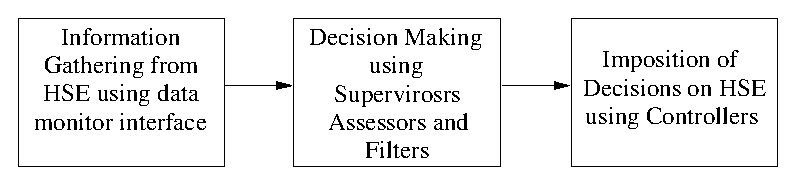
\includegraphics[scale=.85]{Graphics/mseFunctions.eps}
 \end{center}
 \caption{\label{Fig:mseFunctions} Functions of the Management Simulation Engine.}        
\end{figure}

\section{Information Gathering from HSE}

All hydrologic and hydraulic state information including water stages,
flow values, rainfall, ET, hydrologic boundary conditions, or any
other state variable used as input or computed as output by the HSE is
available to the MSE and the assessors through the implementation of a
uniform data monitor interface. The data monitor interface extends
naturally to the MSE input/output variables. Therefore, the input
state information available to a controller or a supervisor is not
limited to water levels or flow values, but can include control
information, decision variables, constraints or any other management
variable from any other assessor or supervisor in the model.  

A central feature of the MSE, which enables decoupling of the
hydrologic state information maintained by the HSE and the operational
process information of the MSE, is the MSE network (Figure
\ref{Fig:mseNetwork}).  This network is based on a standard graph
theory representation of a flow network comprised of arcs and nodes
(Ahuja et al., 1993; Ford and Fulkerson,
1962)\nocite{Ahuja:93}\nocite{Ford:62}.

\begin{figure}
 \begin{center}
  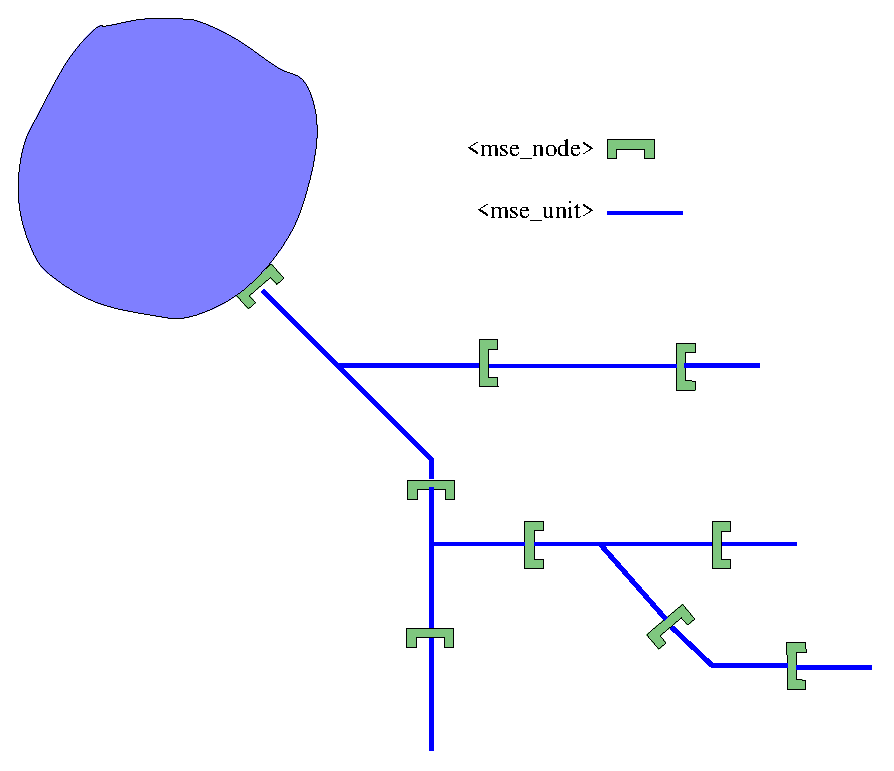
\includegraphics[scale=0.5]{Graphics/mseNetwork.eps}
 \end{center}
 \caption{\label{Fig:mseNetwork} The MSE network structure}        
\end{figure}

From the hydrologic perspective, the HSE canal network is composed of
an interconnected network of segments, with each segment maintaining
parameters relevant to aquifer stream interaction, flow resistance,
spatial coordinates and other physical properties (Figure
\ref{fig:hseNetwork}). The spatial representation of HSE segments is
typically dictated by topographic and physical parameters. From the
water resource management viewpoint of the MSE, the important features
of the flow network are its connectivity, flow capacities, flow
regulation structures, and assessed state information relevant to
managed sections of the network. 

\begin{figure}
 \begin{center}
  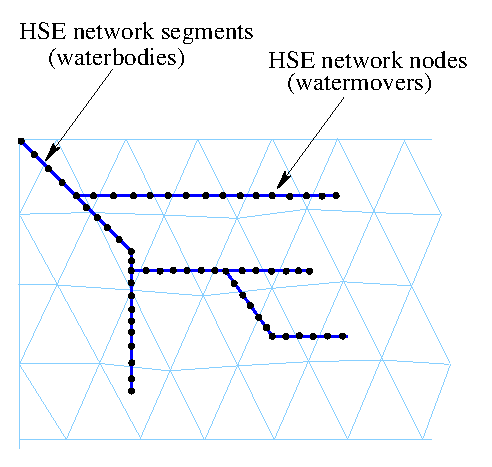
\includegraphics[scale=0.75]{Graphics/hseNetwork.eps}
 \end{center}
 \caption{\label{fig:hseNetwork} The HSE network structure}        
\end{figure}

The primary data object in the MSE network is the water control unit
(WCU). A WCU maps a collection of HSE water bodies that are
operationally managed as a discrete entity in the MSE network. WCUs
are typically bounded by hydraulic control structures, which are
represented as nodes in the MSE network. Each WCU includes associative
references to all inlet and outlet hydraulic flow nodes.

The MSE network data objects serve as state and process information
repositories for management processes. They maintain assessed and
filtered state information, provide parameter storage relevant to a
water control unit (WCU) or hydraulic structure managerial constraints
and variables, and serve as an integrated data source for any MSE
algorithm seeking current state information. Some variables stored in
a structure (node) object include:

\begin{itemize}
 \item current flow capacity of a physical structure
 \item maximum design flow capacity of a physical structure
 \item reference to hydraulic watermover(s) in HSE
 \item reference to structure controller(s) in MSE
 \item operational policy/rule water levels
 \item water supply
 \item water demands
\end{itemize}

The WCU objects incorporate:
\begin{itemize}
 \item time-varying or seasonal stage maintenance levels
 \item flood control stage maintenance levels
 \item inlet flow
 \item outlet flow
 \item water volume
\end{itemize}

Each WCU in the MSE network is referenced by a unique label, and has
an associative data storage object which dynamically allocates storage
for assessment results. This allows multiple, independent assessments
of the WCU state. For example, one assessment of WCU inlet structure
flows might come from a graph algorithm, while another could be
obtained from a LP model.

This abstraction from hydrologic objects to managerial objects
condenses the network representation facilitating the organization and
storage of relevant assessed state and process information. As an
example, Figure \ref{fig:hseNetwork} depicts an HSE canal network
consisting of 63 nodes and 62 segments. Some of the nodes correspond
to locations of hydraulic control structures, though the association
is not apparent from examination of the HSE network. Each canal
segment has a unique identifier which allows the modeler or MSE
processor to monitor state information of the segment. However, it may
be appropriate to make water management decisions based on some
assessed or filtered version of aggregated canal segment states.
Consider now an abstraction of the HSE network into 10 WCUs, regulated
by 11 hydraulic structures, as shown in Figure
\ref{Fig:mseNetwork}. In the MSE network each line segment represents
a WCU, while each node represents a hydraulic structure which
regulates a WCU. The modeler or MSE processor is able to directly
monitor information stored in any of these object data containers,
information which has already been assessed and automatically stored
in the appropriate WCU data object at each timestep.  As with other
RSM model inputs, the WCU mapping from the HSE canal network is
performed with an input XML entry.

The MSE network can also be mapped to basin scale implementations of
the HSE, where regional hydrologic system is simulated by an
interconnected network of basins and lakes, and hydrologic stressors
are applied directly to the basins and lakes through boundary
conditions, rainfall, and ET. The routing of water in the regional
system is governed through operational management policies imposed by
the MSE.  Basin scale implementations have the same important network
flow features (connectivity, flow capacity, etc) as their more complex
distributed mesh/network counterparts.  Water control units are mapped
to basins and lakes and the nodes are mapped to the structures that
provide connectivity between the basins and lakes.

\section{Decision Making: Supervisors, Assessors}

The MSE architecture is based on a multilayered hierarchy, with
individual water control structures regulated by controllers while the
regional coordination and interoperation of controllers is imposed by
supervisors. Supervisors can change the functional behavior of
controllers, completely switch control algorithms for a structure, or
override the controller output based on integrated state information
and/or rules. A schematic depiction of the HSE-MSE layered hierarchy
is shown in Figure \ref{fig:multiLayerHierarchy}.  

\begin{figure}
 \begin{center}
  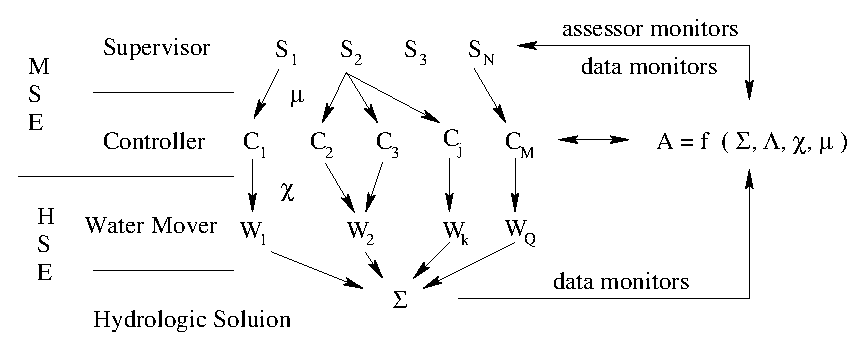
\includegraphics[scale=.85]{Graphics/multiLayerHierarchy.eps}
 \end{center}
 \caption{\label{fig:multiLayerHierarchy} RSM multilayer control hierarchy.}
\end{figure}

At the lowest layer is the hydrologic state information ($\Sigma$)
computed by the HSE. This information includes water stages, flow
values, rainfall, ET, hydrologic boundary conditions, or any other
state variable used as input or computed as output by the HSE. All
such variables are made available to the MSE and assessors through the
implementation of a uniform data monitor interface. This transparency
of state and process information throughout the model is central to
the efficient synthesis and processing of heterogeneous information
required to simplify and naturally express complex water management
policies.  The top level of the MSE is the supervisory layer. There is
no limit on the number of supervisory algorithms, or constraint on the
number of controllers that a supervisor may influence. Based on state
and process information, which optionally may have been filtered or
assessed, the function of a supervisor is to produce the supervisory
control signal ($\mu$) for a single, or collection of, hydraulic
structure controllers. The supervisors are therefore able to
comprehensively coordinate the global behavior of multiple independent
or coupled hydraulic structures.

\subsection{MSE Supervisors}
An MSE supervisor is effectively a meta-controller, a controller of
controllers. The addition of this supervisory layer considerably
simplifies the control expression of multiple, coordinated hydraulic
structures. In addition to the organizational simplification of
control algorithms, the additional layer enables representation of
management functions which are not realizable with a single control
layer.

In relation to the controllers, which are multi-input single-output
(MISO) processors, the supervisors are multi-input multi-output (MIMO)
processors. Supervisors have the ability to change individual response
characteristics of controllers, or, in the case of multiple
controllers attached to a watermover, to dynamically select and
activate a specific controller for any watermover. Specifically, the
supervisory functions include:

\begin{itemize}
 \item Comprehensive assessment of state and process information
 \item Controlling multiple parameters of multiple controllers
 \item Dynamic switching of multiple controllers
 \item Flow regulation override for controller(s)
\end{itemize}

Supervisors can therefore change the functional behavior of
controllers, completely switch control algorithms for a structure, or
override a controller output based on integrated state information
and/or rules.

There is no practical limit on the number of supervisors allowed in a
model, or on the number of controllers that a supervisor may
affect. It is common to have a hybrid selection of different
supervisors, each one regulating a specific sub-regional collection of
hydraulic structures. The ability to selectively tailor management
control algorithms, as well as the flexibility to easily reconfigure
them in a plug-and-play fashion lends considerable power to the
implementation of diverse and complex operational management
scenarios.  The current suite of supervisors includes:

\begin{itemize}
 \item Fuzzy rule based
 \item GLPK Linear Programming (GNU Linear Programming Kit)
 \item Finite state machine (user defined)
 \item Heuristic assessors to capture special operations for a
   particular modeled area
\end{itemize}

These supervisors are discussed in more detail in South Florida Water
Management District (2005) \nocite{sfwmda:2005}.

\subsection{Assessors and Filters}
In the RSM, state and process information can be functionally
transformed by an independent set of filters, which can be viewed as
information pre-processors. These processors are denoted as assessors
and filters. For example, an assessor may perform statistical
filtering such as spatiotemporal expectations, amplitude or time-delay
modulation, or any other suitable data filtering operation. The MSE is
then tasked with appropriately processing the assessed state
information to produce water management control signals, which are
applied to the hydraulic control structures to satisfy the desired
constraints and objectives.  

The role of assessors in the MSE is to perform data preprocessing
required for operational control decisions. By decoupling the
conditioning and filtering of state and process information from the
decision making algorithms, the decision processors can be simplified
and modularized. Therefore, an assessor is an information processor
intended to provide specialized aggregation or differentiation of
state variables particular to a managerial decision process. The suite
of assessors provides for specialized quantification of hydrologic
state variables freeing managerial algorithms from data preprocessing.

Related to the assessors are MSE filters. Filters are generic
information processors implemented to perform simple, often redundant
data filtering operations. The RSM implements a unified design
approach and interface for monitors, filters, and assessors based on
object oriented design principles. As a result, the interfacing of
these constructs from the users perspective is particularly simple and
powerful. Assessor, filters and monitors can operate in a piped FIFO
(first-in, first-out) fashion.

\section{Imposition of Decisions on HSE: Controllers}
The MSE controllers are the intermediary between the hydraulic
structures (watermovers) and the regional-scale supervisory
coordinators. The controllers can operate independently of the
supervisors; in fact, they are not required at all for uncontrolled
operation of a hydraulic structure (e.g., an uncontrolled
spillway). The essential purpose of a controller is to regulate the
maximum available flow through a structure to satisfy a local
constraint. A controller may take as an input variable any state or
process information which can be monitored within the RSM. Since the
interface between a structure watermover and any controller is
uniform, it is possible to change controllers dynamically with a
supervisory command, or manually with a simple XML input change. The
unitary interface also allows for the modeler to mix and match
controllers in a particular model application so that the local
control schemes are a hybridization of any of the available control
algorithms.

At each model time step, once the controllers have computed their
respective control values, these signals are applied as flow
constraints to the structure watermovers in the HSE. Each watermover
will compute a maximum flow capacity based on the hydrologic state
conditions and hydraulic transfer function of the structure. The
resultant controlled flow will be some fraction of the currently
available maximum flow capacity. 


 \section{MSE Assessors}

Assessors were conceived as specialized data processing modules able
to assess, filter and transform individual data into a cohesive,
synoptic assessment of hydrological states used as decision
variables. Recent development has resulted in two implementations of
Assessors: the WCU Assessor, and the WMM Assessor. As a matter of
convenience, these implementations are hybrid Assessor/Supervisor
constructs, they directly control water flows at simulated hydraulic
structures.

The primary function of the MSE Assessors is to estimate the
interbasin management flows which are compatible with the hydrologic
model state response over periods of 1 day, and which satisfy
operational constraints and objectives.  On a regional scale, the
problem is congruent with many historical applications of optimization
techniques aimed at estimating water resource allocations in a
multibasin network flow problem. In the context of the SFRSM this
would include special operations for regional water supply or CERP
projects. 

\subsection{Operational Problem Statement}

Consider a collection of managed basins with controlled flow conduits
between basins. For example, Figure \ref{fig:connectedBasins}
represents a water control network with basins B1 through B6 where
$q_{12}$ indicates the flow from basin B1 to basin B2.

\begin{figure}
 \begin{center}
  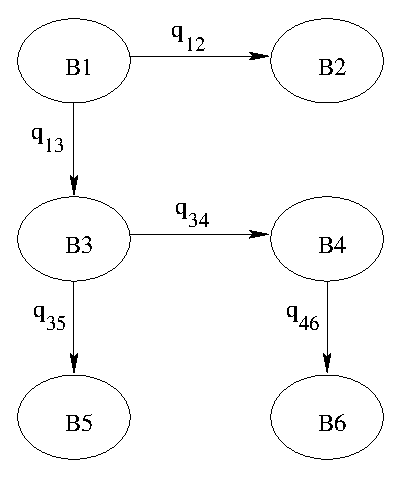
\includegraphics[scale=.75]{Graphics/connectedBasins.eps}
 \end{center}
 \caption{\label{fig:connectedBasins} Water control network of connected basins.}
\end{figure}

In the context of the RSM, a basin consists of a set of:
\begin{itemize}
 \item aquifer/land surface mesh cells, and a collection of canal
   segments or other waterbodies such as lakes, within the confines of
   the basin cells, or
 \item simple basin or lake water body.
\end{itemize}

To facilitate representation of a basin network as a single, managed
water resource, the abstraction Water Control Unit (WCU) refers to the
collection of canal segments within the basin, or the simple basin or
lake waterbody. Each WCU has associated with it a set of operational
constraints. For example a maintenance level specifies a water level
minimum target value for water supply or environmental purposes, while
a flood control level indicates a WCU maximum water level target
value. The flow conduits between basins represent controlled hydraulic
structures. The $q$ values are actually flows between WCU's through a
structure. Each structure may have operational constraints such as a
maximum flow capacity, or maximum/minimum flow values dictated by
water supply or environmental objectives. Functionally, the flow
between two basins depends on both hydrological state information ($s$),
and a managerial control value ($\chi$). The control value is itself a
function of $s$, as well as a function of operational constraints and
objectives ($\lambda$). This can be expressed as:

\begin{align}\label{eqn:interbasinFlow}
 q = f(s,\chi(s,\lambda))
\end{align}

As described in a later section, the state information constitutes
observations of a nonlinear dynamic system.

The flows in Figure \ref{eqn:interbasinFlow} are instantaneous values
which vary continuously, and which we assume are differentiable as
many times as needed. In the context of an RSM implementation used as
a water resource management evaluation or planning tool, the flow
metric of interest is typically a cumulative flow over a period of
time which meets the management objectives. Accordingly, we define the
cumulative flow from basin $n$ to basin $m$ over the time period starting
at $t_s$ and ending at $t_e$ as:

\begin{align}\label{eqn:CumBasintoBasin}
  Q^{se}_{nm} = \int_{t_s}^{t_e}q_{nm}(t)dt
\end{align}

Specifically, in the RSM application to the south Florida region, a
daily timestep has been specified as the simulation increment, i.e.,
$\Delta t = t_e - t_s = 1$ day. This constraint is consistent with a large body
of existing simulation results and database of historical structure
flows and water levels. Further, the model period of record can span
30 years or more, and the large timestep is desirable to limit
simulation run times. However, even at small timesteps on the order of
minutes, the same theory applies. We will denote the cumulative
interbasin flow over a daily time period as $Q_{nm}$. Estimation of the
cumulative flows $Q_{nm}$ over a simulation timestep of 1 day is the
primary objective of the WMM Assessor (Section 2.4), and of the linear
programming models which are under development (Sections 2.7 and 2.8).

\subsection{RSM State Estimation}

RSM is a state estimator. We denote estimates of variables with
italics. RSM allows independent abstraction of hydrological and
managerial state variables through the interoperation of the
Hydrologic Simulation Engine (HSE) and the Management Simulation
Engine (MSE). HSE provides hydrologic state evaluations, $s$, while
MSE facilitates estimation of controlled variables such as
$q_{nm}$. RSM also provides for transformation of $s$ with a set of
data filters known as Assessors. A schematic of the overall RSM state
information cyclic flow is shown in Figure \ref{fig:rsmSchematic}.

\begin{figure}
 \begin{center}
  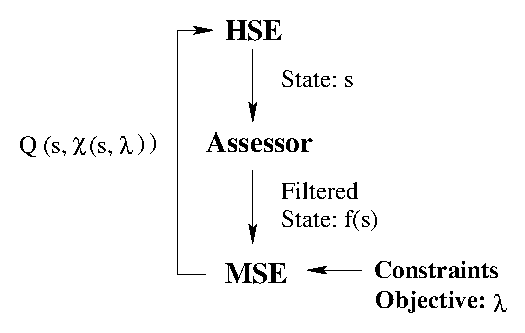
\includegraphics[scale=.75]{Graphics/rsmSchematic.eps}
 \end{center}
 \caption{\label{fig:rsmSchematic}  RSM schematic}
\end{figure}
 
\subsubsection{Linear Model}

HSE facilitates estimation of the hydrological states through a
linearized diffusion flow formulation. Typically, a linear model is
represented as a superposition of weighted states and forcing (or
basis) functions:
\begin{align}\label{eqn:linearModel}
  s(n) = \sum_{i=1}^{N}a_is(n-i) + \sum_{j=1}^Mb_j\Phi(n-j)
\end{align}

where $a_i$ and $b_j$ are model coefficients and $\Phi$ represent the
forcing terms. The task is then one of judiciously selecting the
coefficients to conform the model results to the observations. In HSE
[SFWMD1, 2005], the hydrologic representation is

\begin{align}\label{eqn:hseHydroRep}
 \mathbf{A}(\mathbf{H}) \cdot \frac{d\mathbf{H}}{dt} = \mathbf{q}(\mathbf{H}) + \mathbf{S}(\mathbf{H})
\end{align}

where $\mathbf{H}$ is a vector of finite volume waterbody states,
$\mathbf{q(H)}$ is a vector containing the summation of flow entering
the waterbodies, $\mathbf{S(H)}$ are non-gradient driven fluxes (source
terms) and $\mathbf{A(H)}$ is a diagonal matrix whose elements contain
the effective areas of the waterbodies. The flows $\mathbf{q(H)}$ are
linearized through use of a global flow resistance matrix
$\mathbf{M(H)}$:

\begin{align}\label{eqn:flowMatrix}
 \mathbf{q}(\mathbf{H}) = \mathbf{M}(\mathbf{H}) \cdot \mathbf{H}
\end{align}

The flows of equation \ref{eqn:flowMatrix} are solved with a PETSC
sparse linear system solver [SFWMD1 2005]. Once a solution of the
hydrologic states is available, dynamic evolution of the simulation is
specified as

\begin{align}
  s(n+1) = s(n) + \mathbf{A_n} \cdot \Delta \mathbf{H}
\end{align}

which is a special case of equation \ref{eqn:linearModel}. 

While many of the linearizations are well characterized, it is
possible that state variable regimes which invalidate the linear
assumptions could precipitate unanticipated model behaviors. The
chosen spatiotemporal discretizations of the model representation are
also capable of introducing nonlinear simulation artifacts. In
addition, there are likely nonlinear system variables which are
ignored by the model equations. Further, there may be inherent
limitations in the exclusion of hydrodynamic momentum terms from the
model formulation wherein stream flow dynamics are approximated. It is
known that the hydrological states are expressions of the dynamic
evolution of a nonlinear, chaotic timeseries [Park 2005], however, the
significant dissipation inherent in the physical system allows
reasonable approximations given well behaved linearizations ($ds/dt\ 
\alpha\ t$) and small enough simulation timesteps ($\Delta t \to$ 0).

\chapter{WMM Assessor}

The Water Management Model (WMM) Assessor refers to a combined state
variable assessor and interbasin water flow supervisor. It is based on
methodology implemented in the South Florida Water Management Model
(SFWMM)[SFWMD, 1999]\nocite{sfwmm:99}, and on code from the WCU
Assessors. The WMM Assessor estimates controlled basin structural
outflows to satisfy both water supply and flood control operational
constraints.

The WMM Assessor is designed to estimate the cumulative flows $Q_{nm}$
over a simulation timestep of one day. Currently, this is done through
an iterative procedure which updates state information from the HSE
for refined flow estimates in the WMM Assessor. This section documents
the WMM Assessor that is implemented for the SFRSM project.

\section{Assess Flow Function}\label{assessFunction}

The WMM Assessor interface in the RSM is contained in the Assess()
function. A flowchart schematic representation of this function is
shown in Figure \ref{fig:flowchartWMM}

\begin{figure}
 \begin{center}
  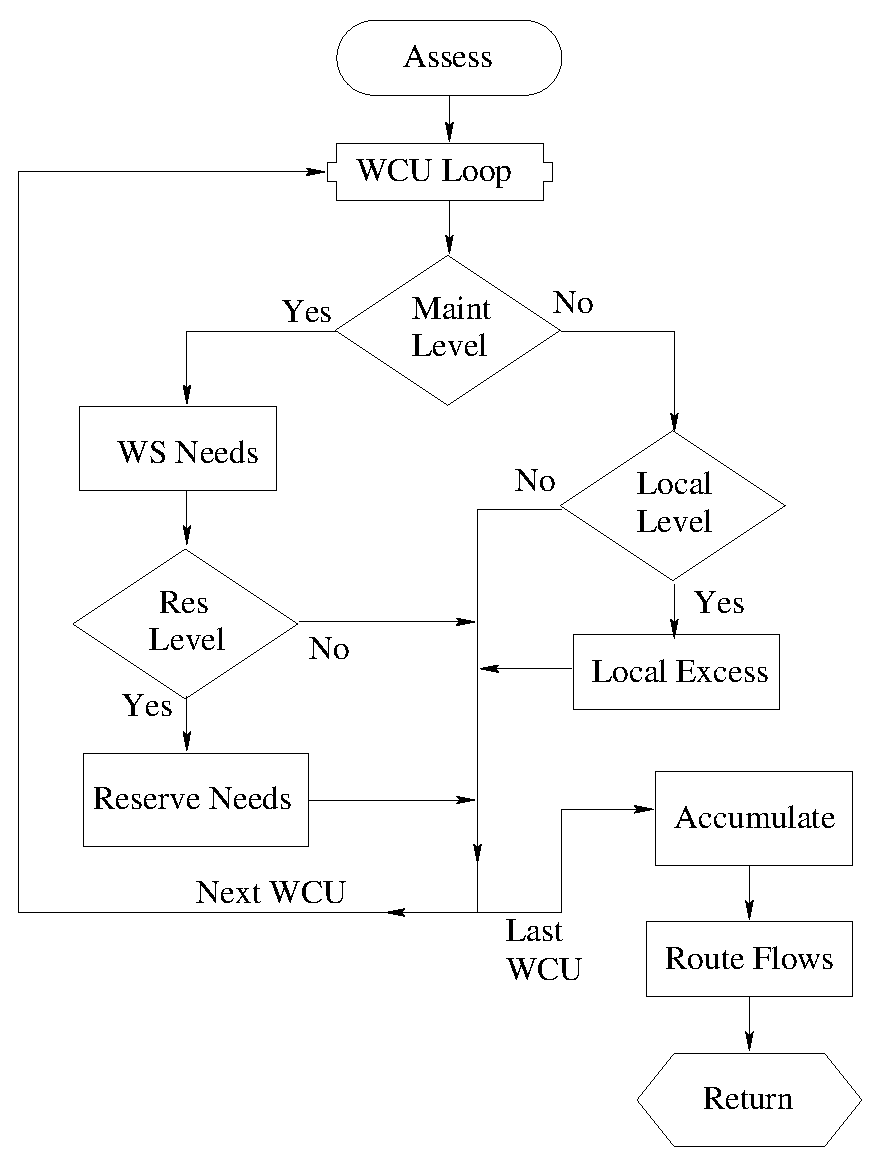
\includegraphics[scale=.33]{Graphics/flowchartWMM.eps}
 \end{center}
 \caption{\label{fig:flowchartWMM} Flowchart of WMM Assessor main
   function; Assess()}
\end{figure}

The Assess() function is executed before each solution of the HSE
state equations. Once the WCU outlet flows ($Q_{nm}$) are estimated,
these flows are imposed as boundary conditions on the HSE
solution. The Assess() function has three primary operations:

\begin{enumerate}
 \item Assess the volumetric supply or demand (needs) of each WCU 
 \item Accumulate the WCU needs across multiple, interconnected WCUs 
 \item Route WCU outlet flows to satisfy water supply needs and flood
   control objectives
\end{enumerate}

The water supply needs are evaluated by the three functions WSNeeds(),
ReserveNeeds() and LocalExcess(). These three functions perform
essentially the same computation: estimate the volume of water needed
to raise or lower a WCU to a target level, but with respect to three
different target water levels: MaintLevel, ResLevel and LocalLevel
respectively. The function which computes the water supply needs for
each target is the TargetVolume() function.

WSNeeds() is the volume of water required to bring the downstream end
of a WCU to its maintenance level. ReserveNeeds() is a smaller volume
than WSNeeds() and is the volume that will be supplied to a WCU if
water availability from upstream sources is limited. LocalExcess() is
the volume that a flow-thru WCU can provide as local water supply to
downstream WCUs. If a flow-thru WCU has excess volume, LocalExcess()
will return a negative volume.

\section {TargetVolume() function}

The primary computation of the TargetVolume() function is an estimate
of the total volumetric water differential needed to raise or lower
the water level of a WCU to satisfy a target water level. This
computation is specific to water supply needs or excesses, flood
control releases are computed separately in the RouteFlow() function.

Figure \ref{fig:WCUvolumeTarget} indicates a cross-sectional view of a
WCU consisting of four HSE canal segments. The water level difference
between the initial level and the target level at the downstream
control point is denoted $\Delta HT$. Once this target differential is
computed, it is added as an offset to each canal segment water level
in the WCU. These \emph{adjusted} water levels constitute a WCU water
level profile which defines the target water levels over the entire
WCU.

\begin{figure}
 \begin{center}
  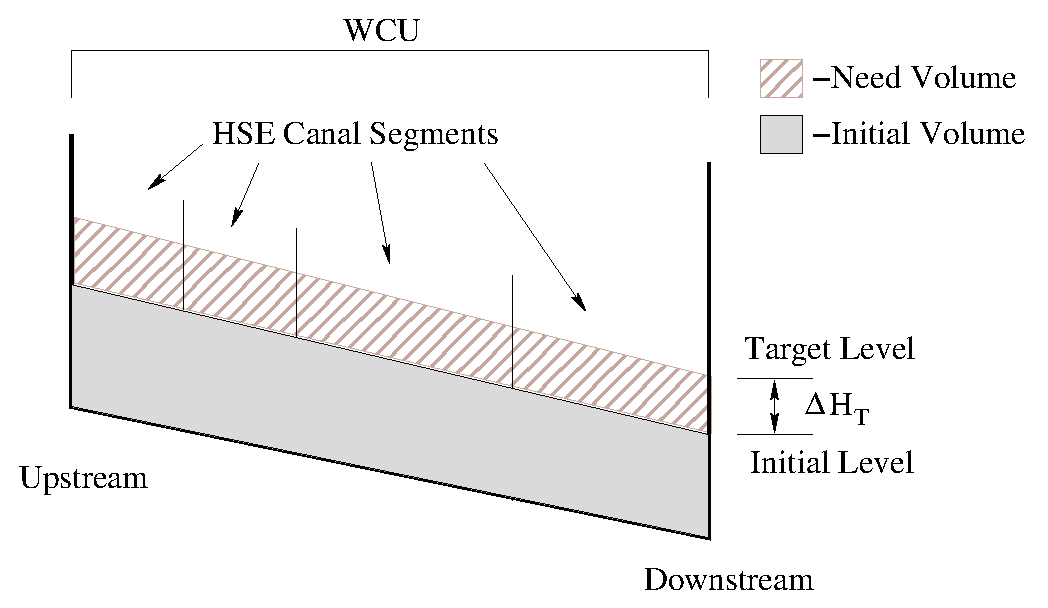
\includegraphics[scale=.5]{Graphics/WCUvolumeTarget.eps}
 \end{center}
 \caption{\label{fig:WCUvolumeTarget} WCU volume and target level for
   water supply needs}
\end{figure}

In the first HSE iteration, it is assumed that the target profile is
parallel to the previous time step profile. However, in subsequent
iterations, the target profile is assumed parallel to the profile
obtained in the previous sub-timestep iteration. 

Once the adjusted target profile is available, each canal segment in
the WCU is processed to estimate:

\begin{enumerate}
 \item Volume required to raise/lower the initial level to the target:
   $V_{H_t}$
 \item Canal segment water stage: $s_s(n) = s_s(n - 1) + \alpha_h \Delta H$ 
 \item Aquifer cell water stage: $s_c(n) = s_c(n - 1) + \alpha_h\Delta H$ 
 \item Volume of canal/aquifer seepage: $V_{SP} = f(s_s(n), s_c(n))$ 
 \item Volume canal overbank flow: $V_{OB} = f(s_s(n), s_c(n))$ 
 \item Volume of levee seepage: $V_{LV} = f(s_s(n), s_c(n))$ 
 \item Volume of boundary condition flows: $V_{BC}$ 
 \item Volume of WCU unmanaged (passive) structure inlets: $V_I (s_s(n))$ 
 \item Volume of WCU unmanaged (passive) structure outlets: $V_O(s_s(n))$
\end{enumerate}
 
where $s_s$ is the canal segment water level, $s_c$ the aquifer cell
water level, $a_h$ an implicit/explicit numerical solution weight
(SFWMDb, 2005)\nocite{sfwmdb:2005}, and $\Delta H$ the previous HSE
solution of state change. Boundary condition flows include HSE
watermovers defined by HSE boundary conditions, for example, a canal
segment may have a water stage boundary condition, or flow boundary
condition defined by a timeseries (SFWMDb,
2005)\nocite{sfwmdb:2005}. These estimates are then accumulated into a
final value of volumetric water supply need (WSN) for the WCU:

\begin{align} \label{eqn:wsn}
  V_{WSN} = \sum_{i=1}^{N} (V_{H_{T_i}} + V_{SP_i} + V_{OB_i} + V_{LV_i} + V_{BC_i} + V_{I_i} + V_{O_i})
\end{align}

where $N$ is the total number of canal segments in the WCU. The value
of $V_{WSN}$ is contained within the domain of $\Re$. Positive
$V_{WSN}$ indicates the deficit volume which needs to be added to the
WCU to meet the target level, negative $V_{WSN}$ signifies a volume of
excess water above the target level. The estimates of $V_{WSN}$ are
stored in data objects of each respective WCU for subsequent
reference.

\section {Accumulate() function}

After each WCU has been evaluated for water supply needs, the
Accumulate() function processes the entire WCU network to estimate the
cumulative water supply need at each WCU inlet. Figure
\ref{fig:flowchartAccumulate} depicts a schematic flowchart of the
Accumulate() function.

\begin{figure}
 \begin{center}
  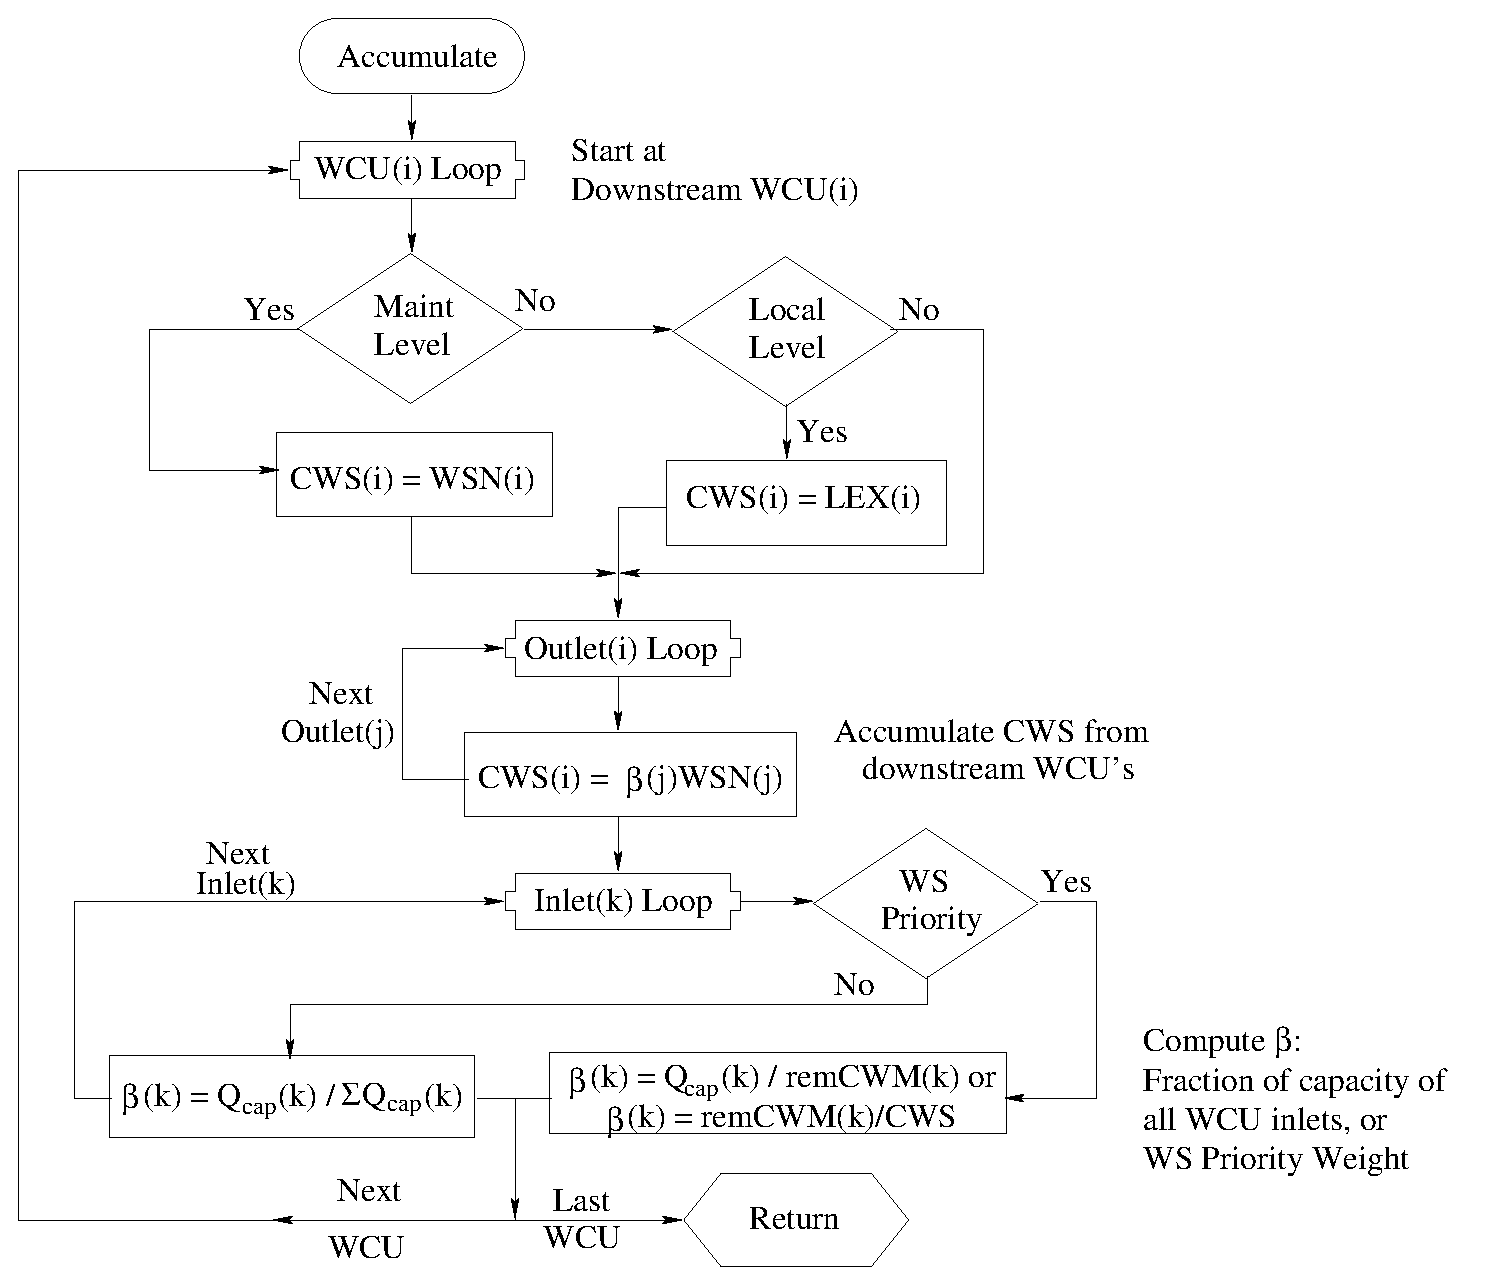
\includegraphics[scale=.33]{Graphics/flowchartAccumulate.eps}
 \end{center}
 \caption{\label{fig:flowchartAccumulate} Flowchart of WMM Assessor function; Accumulate()}
\end{figure}

The Accumulate() function contains three internal loops: 
\begin{enumerate}
 \item Process all WCUs from downstream to upstream (index(i)) 
 \item Process all outlets of a WCU to accumulate the CWS (index(j)) 
 \item Process all inlets of a WCU to compute capacity weight $\beta$
   (index(k)), or to set the water supply priority fraction of CWS for
   each inlet.
\end{enumerate}

The first (outer) loop ensures that all WCUs in the flow control
network are processed. The order of processing is determined by the
structure of the MSE Network definition file (SFWMDc,
2005)\nocite{sfwmdc:2005}. The first step in this loop is to
initialize the cumulative water supply need (CWS) for each WCU as
either the water supply need (WSN, positive or negative) or local
excess (LEX, negative) volume which were previously computed for each
WCU according to equation \ref{eqn:wsn} (see Figure
\ref{fig:flowchartWMM}).

The second loop then accesses all water supply outlet structures of
the current WCU, and accumulates their downstream CWS with the current
WCU. This accumulation is weighted by the flow capacity of the
downstream outlet structures. CWSj is limited to being greater than or
equal to 0, since excess water cannot be transferred upstream. The
third loop computes the a structure flow weight $\beta$ for all water
supply inlets of the current WCU. Since the processing of WCUs is from
downstream to upstream, a value of $\beta$ is always available for WCU
outlets in the second loop. $\beta$ is used for WCUs with multiple
water supply inlets to assign fractions of CWS to be met through
different routes. Computation of ß can be done in one of two modes. In
the default mode, the assumption is that routes with more capacity
will be used proportionally more for water supply, and therefore the
value of $\beta$ is simply a fraction of total WCU inlet capacity for
each inlet. Alternatively, if the WSPriority option is specified, then
each inlet is assigned an integer WSPriority value, lower integers
have higher priority. In this case, $\beta$ is computed to accommodate
available WS capacity for each inlet in order of priority, until the
WCU CWS needs are met.

\section {RouteFlow() function}

The functions described previously all fall under the functional
classification of assessors, they perform data filtering and
processing of state information to facilitate a decision
process. RouteFlow performs assessment functions, however it also
performs supervisory functions: it makes decisions on operational
flows imposed at flow control structures. A schematic flowchart of the
RouteFlow function is presented in Figure \ref{fig:flowchartRouteFlow}.

\begin{figure}
 \begin{center}
  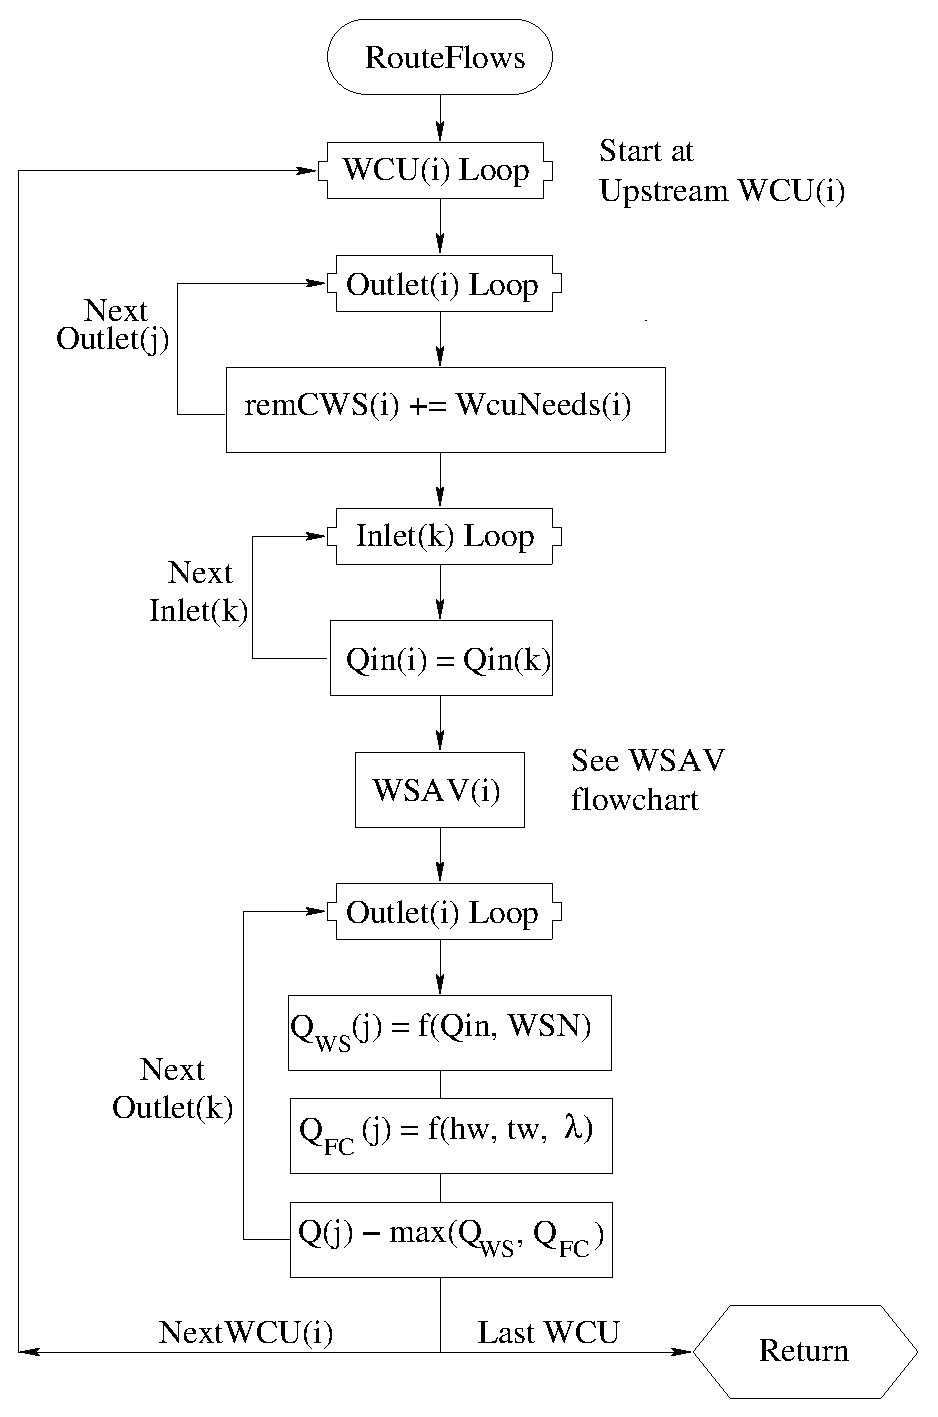
\includegraphics[scale=.33]{Graphics/flowchartRouteFlow.eps}
 \end{center}
 \caption{\label{fig:flowchartRouteFlow} Flowchart of WMM Assessor function: RouteFlow()}
\end{figure}
 
RouteFlow has a main (outer) loop which processes all WCUs starting at
the most upstream point, and sequentially progressing to the most
downstreamWCU as defined in the MSE Network definition file (SFWMDc,
2005)\nocite{sfwmdc:2005}. Since there is no recursive processing
involved, RouteFlow is not capable of balancing needs and flows that
change as a result of the flow decisions made in the single-pass
linear processing of WCUs. One of the ways in which this issue is
currently addressed is through the use of HSE-MSE iterations.

The following descriptions are with respect to a single WCU. The first
assessment in RouteFlow computes the remaining cumulative water supply
needs ($remCWS_i$) of the current WCU based on WCU outlets that are
designated as being Water Supply control structures. The computation
for a WCU with index $i$ that has water supply outlets with index $j$
is:

\begin{align}
  remCWS_i = \sum_j^N \beta _j CWS_j
\end{align}

Once the cumulative downstream needs have been compiled, the water
supply needs (WSN) for the WCU is computed by adding the local WCU WSN
to the $remCWS$:

\begin{align}
  CWS_i = WSN_L + remCWS_i
\end{align}

where $WSN_L$ represents the local WSN computed in Assess(). 

The next assessment to accumulate the total inflow from WCU inlet
structures, these individual values were computed previously for the
WCUs immediately upstream of the current WCU:

\begin{align}
  Q_{in_i} = \sum_j^N Q_k
\end{align}


Followed by a conditional assessment of the water supply available
volume (WSAV) based on cumulative structural inflows. $Q_{in_i}$  is converted to
a water supply available volume ($WSAV_i$) as follows:

\begin{align}
  WSAV_i = Q_{in_i} \Delta t
\end{align}

A schematic flowchart of $WSAV_i$ computation is shown in Figure
\ref{fig:flowchartWSAV}. Figure \ref{fig:flowchartWSAV} shows how
$WSAV_i$ is decremented as portions of it are assigned to the current
WCU and to downstream WCUs. These assignments depend on the purpose of
the current WCU and the magnitude of WSAV compared to needs.

\begin{figure}
 \begin{center}
  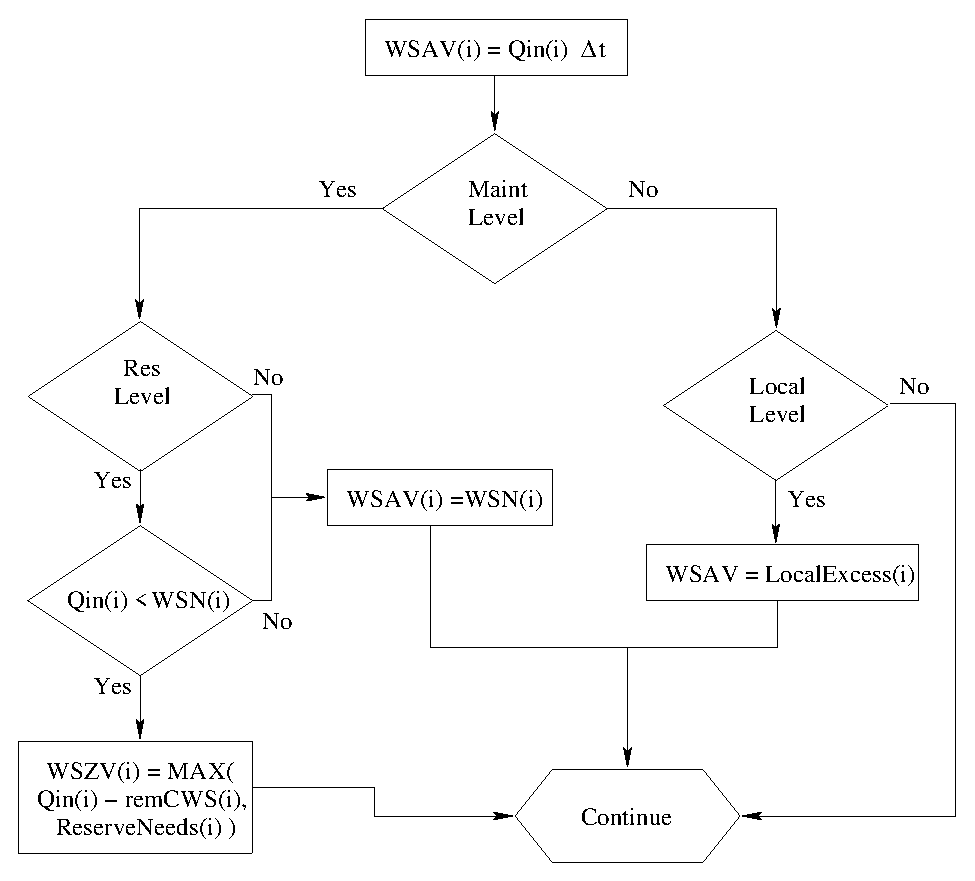
\includegraphics[scale=.33]{Graphics/flowchartWSAV.eps}
 \end{center}
 \caption{\label{fig:flowchartWSAV} Flowchart of Water Supply Available Volume (WSAV) in RouteFlow() function}
\end{figure}

If the currentWCU has a maintenance level but no reserve level, then
the first priority is to meet needs in the current WCU. Any remaining
portion of $WSAV_i$ will be available to meet needs in downstream
WCUs. If the current WCU has a maintenance level and a reserve level,
and there is not enough water available to meet all needs (i.e.,
$WSAV_i < CWS_i$), then only a portion of this WCU's needs are
met. The portion corresponds to at least the reserve level volume if
available. The remaining portion of $WSAV_i$ is available for
downstream WCUs. If the current WCU has local excess, it is added to
the available volume from upstream (i.e., a negative value is
subtracted from $WSAV_i$). For flow-through WCUs, all of $WSAV_i$ will
be available to meet needs in downstream WCUs.

Accordingly, WSAV can be expressed as: 
\begin{align}
 WSAV_i = \left\{
  \begin{array}{l l}
    Q_{in_i} \Delta t; & \quad initialvalue \\
    WSAV_i - MIN(WSAV_i, MAX(Q_{in_i}\Delta t - remCWS_i, ResNeeds_i)); & \quad ResLevel \\
    WSAV_i - WSN_i &\quad MaintLevel \\
    WSAV_i - LEX_i; & \quad LocalLevel \\
  \end{array} \right.
\end{align}


where LEX represents the Local Excess (negative) volume computed by LocalExcess(). 

\section{WS Flow Computation}
At this point in the RouteFlow() function the accumulated assessments
are completed, the processing now shifts to a supervisory mode wherein
the outlet flows are computed for each outlet of the respective WCUs.

The water supply (WS) flow for each water supply outlet structure is
based on the available volume of water in the WCU that can be used to
meet the cumulative downstream water supply needs. For each WS outlet
of the WCU, the available volume (AV) is computed according to a
shared adversity assumption:
\begin{align}
  AV_J &= (WSAV_j / remCWS) \cdot \beta_j &remCWS &> 0
\end{align}

where $CWS_j$ is the cumulative water supply need downstream of the
outlet.

The outlet WS flow for the structure with index j is specified as: 
\begin{align}
 Q_{WS_j} = MIN ( Q(hw, tw), AV_j / \Delta t)
\end{align}

where Q(hw, tw) is the current state flow capacity reported by the HSE
watermover. Note that hw and tw are the latest state estimates from
the previous HSE solution, these values may be from sub-timestep
iterations. The value of $Q_{WS}$ is then limited by the design
capacity of the structure.

The final step of the WS computation is to decrement the remCWS: 
\begin{align}
  remCWS_i \text{ -= } CWS_j \cdot \beta_j
\end{align}

and to decrement the WSAV of the WCU: 

\begin{align}
  WSAV_i \text{ -= } Q_{ws_j} \cdot \Delta t
\end{align}

\section{FC Flow Computation}

Flood control (FC) flows are based on water levels with respect to the
flood control criteria specified for each WCU outlet structure. The
criteria are expressed as an open and close water level. The FC flow
is:

\begin{align}\label{eqn:FCflow}
  Q_{FC_j} = \gamma_j \cdot Q_j(hw, tw)
\end{align}

where $\gamma$ represents a fractional value of total flow. $\gamma$
is based on a fractional gate opening for the structure fracGO:

\begin{align}
  fracGO = \frac {hw - close}{open - close}
\end{align}

 is computed as a power function (SFWMD, 1999).\nocite{sfwmm:99} 

\begin{align}
  \gamma = fracGO^b
\end{align}

where $b$ is a parameter usually set to 2. The resultant value of $Q_{FC}$
is limited by the design flow capacity of the outlet structure.

\section{Flow Assignment}
Once estimates for the WCU outlet water supply and flood control flows
are available, the final outlet flow value is simply a maximum of the
two values:
\begin{align}
  Q_j = MAX(Q_{WS_j}, Q_{FC_j})
\end{align}

This value is imposed as a boundary condition on the HSE solution of
Equation \ref{eqn:flowMatrix} for the structure watermover between the
respective WCU canal segments.

\section{MSE - HSE Convergence}\label{InfoMismatch}
A distinguishing feature of the HSE is the fully integrated
aquifer-stream flow solution. The finite volume hydrological
formulation expressed in Equation \ref{eqn:hseHydroRep} is solved in
one step (Equation \ref{eqn:flowMatrix}) for all waterbodies in the
model, inclusive of canal segments and aquifer cells. The HSE solution
is therefore an integrated global solution of the simulation
hydrologic processes. This feature is desirable from a physical
modeling perspective, as the physical system reacts as a global,
unitary, fully coupled system.

However, it is problematic from the point of view of MSE which
computes watermover flows independently of the conjunctive HSE
solution. The essential difficulty is that the MSE decisions are based
on previous HSE solution state information, but are imposed on the
next HSE solution as flow boundary conditions. As the simulation
timestep duration increases ($\Delta t = t_e - t_s$ of Equation
\ref{eqn:CumBasintoBasin} becomes large) the divergence between the
actual cumulative flow $Q_{mn}$, and the flow estimated by the WMM Assessor
$Q_{mn}$ increases. This divergence arises for several reasons:

\begin{enumerate}
  \item $Q_{mn}$ is based on previous timestep state information. 

  \item Nonlinearities approximated in the global HSE solution of the
    equations are not modeled in the WMM Assessor.

  \item Lack of synoptic (multipleWCU) balancing of headwater and
    tailwater in the WMM Assessor.
\end{enumerate}

An observational result of this divergence is the WCU Profile Mismatch
which precipitates canal stage \emph{oscillations}. 

\section{WCU Profile Mismatch}
Consider a coupled set of upstream-downstream WCUs with a single
controlled flow structure between WCUs as illustrated in Figure
\ref{fig:wcusCoupled}. Each WCU has MSE controlled structural inflow
and outflow, for example structure $S_{01}$ controls flow $Q_{01}$
into $WCU_1$, and structure $S_{12}$ controls flow $Q_{12}$ out of
$WCU_1$ into $WCU_2$. These cumulative structural flows are estimated
by the WMM Assessor. Each WCU is also subjected to boundary
condition and hydrologic state influenced inflows and outflows ($Q_s$)
which include aquifer-canal seepage, rainfall, and all other
non-structural fluxes. Operational criteria for a WCU can include a
water supply maintenance level $T_{WS}$, and flood control level
$T_{FC}$ specified at the downstream end of a WCU.

 \begin{figure}
 \begin{center}
  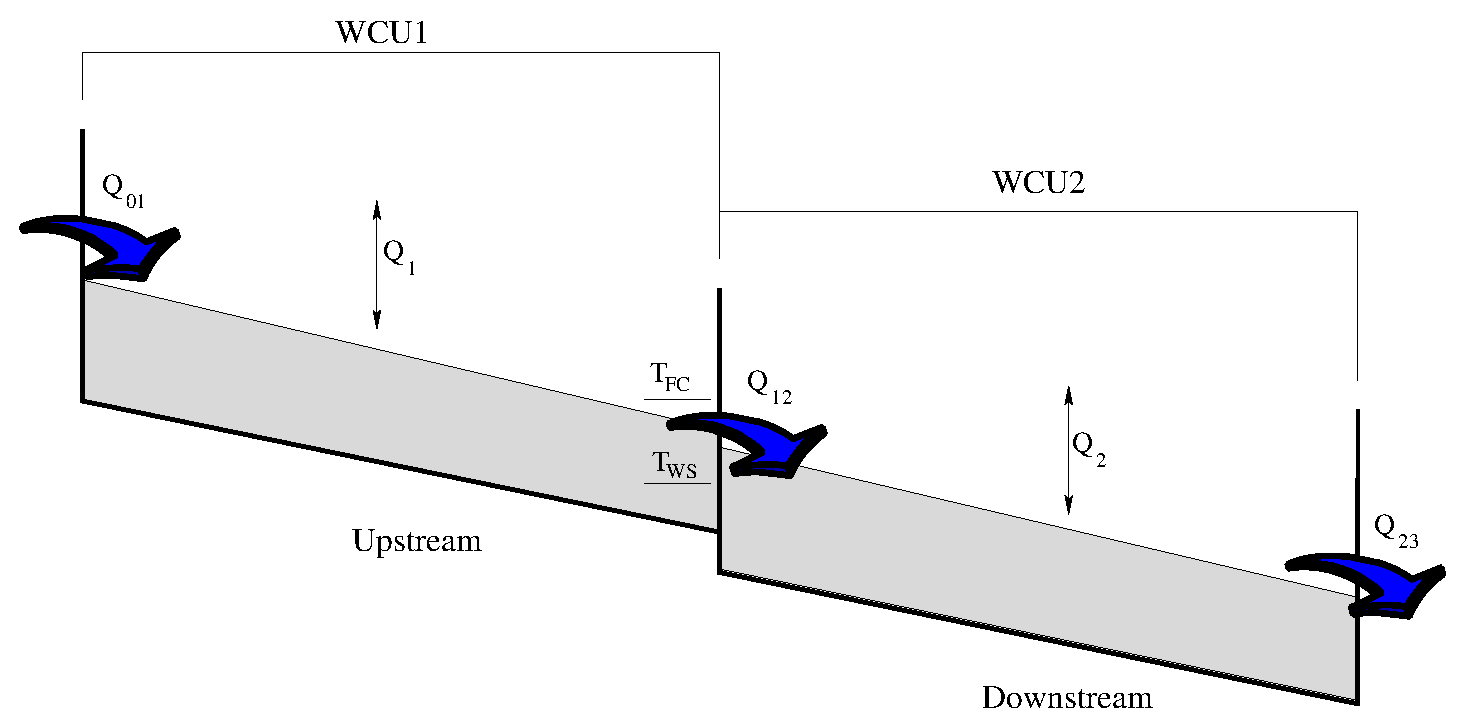
\includegraphics[scale=.33]{Graphics/wcusCoupled.eps}
 \end{center}
 \caption{\label{fig:wcusCoupled} Two WCUs coupled by a structure with flow $Q_{12}$}
\end{figure}

Interbasin flow estimates for the next timestep ($Q_{12}(n + 1)$) are
based on previous timestep information ($s(n),Q_s(n)$) and are likely
to differ from the actual flows $Q_{12}(n + 1)$. Further, these
estimates are imposed as flow boundary conditions on Equation
\ref{eqn:flowMatrix} for the next timestep (n+1) solution. The
imposition of an erroneous estimate can produce significant impacts on
the global hydrologic solution. In the case of a positive residual
$\Delta Q_{12} = Q_{12} - Q_{12} > 0$; where the estimated flow is
less than the ideal flow, the upstream WCU will contain excess water
and will result in a $WCU_1$ water level profile that is higher than
that \emph{expected} by the ideal solution. The deficit of transfer
flow from $WCU_1$ to $WCU_2$ will also result in a lower water level
in $WCU_2$ than would occur with the correct flow value. This
situation is depicted in Figure \ref{fig:wcusCoupled_1}.

 \begin{figure}
 \begin{center}
  \includegraphics[scale=.33]{Graphics/wcusCoupled_1.eps}
 \end{center}
 \caption{\label{fig:wcusCoupled_1} WCU state if estimated flow $Q_{12}$ is less than actual $Q_{12}$.}
\end{figure}

As a result of the positive flow residual, the headwater of structure
$S_{12}$ is above that of the correct value while the tailwater is
below the expected value. This increased head differential will
produce a larger potential structure flow (the flow produced by
application of the structure watermover transfer function to the
applied headwater and tailwater) than the correct value. These
erroneous water levels and the incorrect potential flow will be used
in the next timestep. Another issue concerns the flood control target
level of $WCU_1$. The estimated WCU water level exceeds the flood
control level, while the correct value does not. The result would be
an incorrect flood control flow release for structure $S_{12}$.

Consider now a negative flow residual: $\Delta Q_{12} = Q_{12} -
Q_{12} < 0$; where the estimated flow is greater than the actual flow,
the resultant WCU water levels could be as shown in Figure \ref{fig:wcusCoupled_2}.

 \begin{figure}
 \begin{center}
  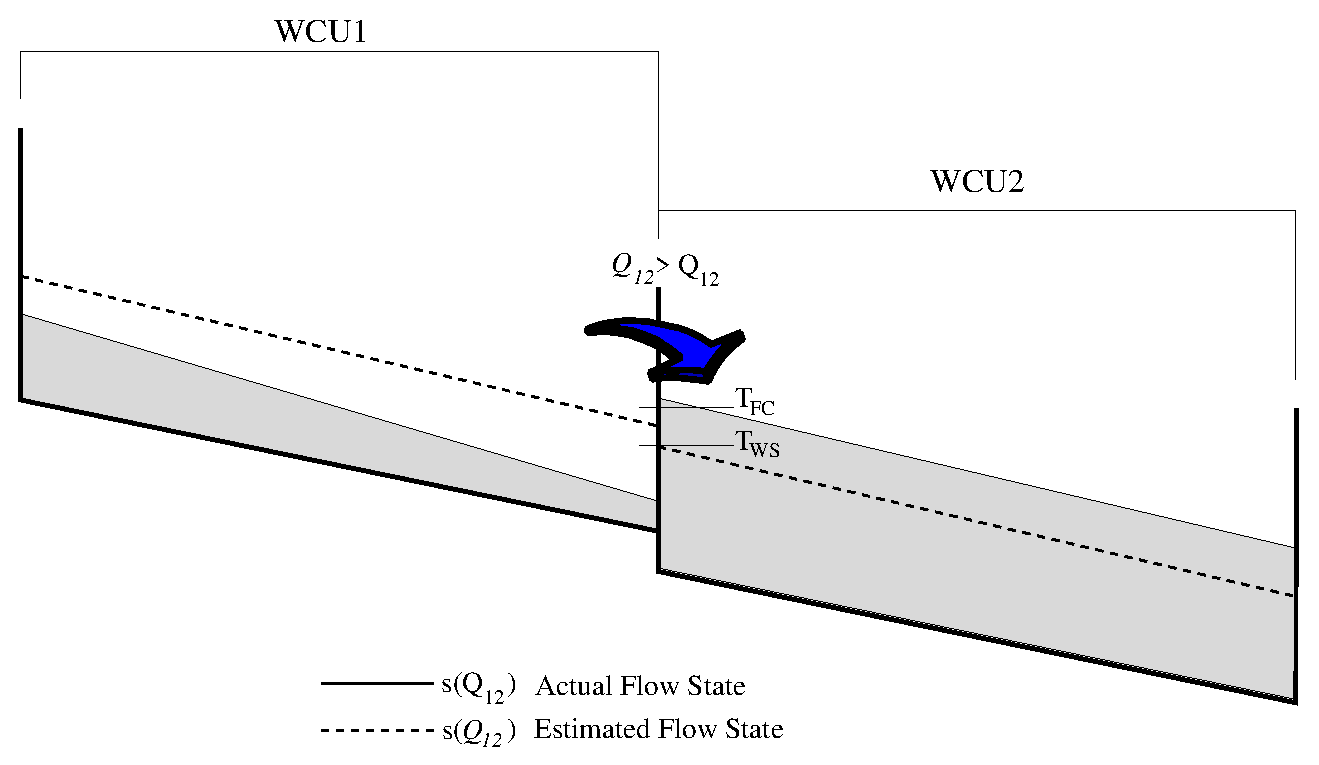
\includegraphics[scale=.33]{Graphics/wcusCoupled_2.eps}
 \end{center}
 \caption{\label{fig:wcusCoupled_2} WCU state if estimated flow $Q_{12}$ is greater than actual $Q_{12}$.}
\end{figure}

The negative flow residual has created a water level inversion, the
tailwater of structure $S_{12}$ is above the headwater. The potential
flow of the structure will be zero. The resultant water level in
$WCU_1$ can also fall below the water supply threshold, whereas the
actual value would not. The erroneous potential flow and threshold
crossing will result in incorrect flow computations on the next
timestep.

\section{MSE Induced Oscillation}
There are many causes of canal water level oscillations in hydraulic
numerical models, for example, improper spatiotemporal
discretizations, numerical threshold crossings, or uncompensated
control signals applied to hydraulic flows.

Consider the situation presented in Figure \ref{fig:wcusCoupled_1}
where the WMM Assessor encounters a water level in $WCU_1$ above the
flood control threshold $T_{FC}$. The reason for this water level,
whether through estimation inaccuracy or levels match the actual
values, is not germane. The WMM Assessor will compute a flood control
release flow according to Equation \ref{eqn:FCflow}. This value of
$Q_{12} = Q_{FC}$ will be relatively large with respect to the
structure flow capacity. The large flow can result in significant
reduction of water level in $WCU_1$ for the next timestep, lowering
the level below the flood control threshold analogous with Figure
\ref{fig:wcusCoupled_2}. After the next timestep the $WCU_1$ level may
be low enough that no flow release is warranted, thereby setting
$Q_{12} =0$. If the upstream structural and other inflows ($Q_{12} + Q_s$)
are significant enough, then in the following timestep the levels in
$WCU_1$ may again rise above $T_{FC}$, and the cycle repeats.

This cyclic recurrence of control limit states, $\Delta Q_{12} =
Q_{FC}; Q_{12} = 0$, is commonly referred to as \emph{bang-bang}
control, or \emph{slamming}. The controller is slamming between
maximal control points due to saturation of the control input state
variables. Typical solutions entail filtering of the input states,
and/or incorporation of an integration term in the control
algorithm. In the current WMM Assessor implementation, an alternative
approach is used where a convergence function is applied to limit the
changes in estimated interbasin flow ($Q_{mn}$) so that a global
solution can be found based on HSE state information feedback.

Even though slamming appears to the primary cause of observed canal
oscillations, and this limit cycle behavior is certainly dependent on
the nonzero flow estimate residuals, it is possible that the
inaccuracies and nonzero flow estimate residuals themselves can
produce oscillations as described in Section \ref{InfoMismatch}.

\section{MSE - HSE Iterations}
Recognizing that the WMM Assessor estimated flow residuals diverge as
the simulation timestep increases, a natural solution is to provide
iterative HSE state information updates in in order to refine the
estimated flows within a timestep. An error metric which quantifies
the flow estimate divergence is used to terminate the iterations when
a convergence threshold is satisfied. RSM performs this iterative flow
refinement in three basic steps:

\begin{enumerate}
  \item WMM Assessor estimates flows $Q_A$ based on the latest HSE
    iteration state information ($\Sigma (j-1)$) and management constraints
    ($\lambda$).

  \item Estimated flow ($Q_A$) changes are limited with a convergence
    function to produce the final estimated flow $Q$.

  \item New HSE state estimates are solved by imposition of the
    estimated flows $Q$ applied to previous timestep state conditions
    ($\Sigma (i)$).
\end{enumerate}

A schematic flowchart of the MSE - HSE iteration is shown in Figure
\ref{fig:flowchartIteration}. Referring to Figure
\ref{fig:flowchartIteration}, there are two processing loops
shown. The outer loop represents a HSE timestep and is indexed with
the variable $i$. As i changes from $i$ to $i+1$, the HSE simulation has
advanced forward by one timestep ($\Delta t$). The inner loop depicted in
Figure \ref{fig:flowchartIteration} is the MSE - HSE iteration loop,
it is represented with the iteration index $j$.

\begin{figure}
 \begin{center}
  \includegraphics[scale=.33]{Graphics/flowchartIteration.eps}
 \end{center}
 \caption{\label{fig:flowchartIteration} Schematic flowchart of
   HSE-MSE iteration algorithm.}
\end{figure}

The first computation estimates the desired flow QA based on the
latest state information which will satisfy the operational
constraints, thus:

\begin{align}
  Q_A = m [ \Sigma (j - i), \lambda ]
\end{align}

where m[] indicates the WMM Assessor processing described in Section
\ref{assessFunction}. The argument $\Sigma(j-1)$ refers to the HSE
state information obtained from the previous (latest) HSE iteration,
and as before $\lambda$ refers to the managerial constraints such as
WCU target levels for water supply and flood control. Therefore, the
first step consists of estimating the flows required to meet the
operational constraints where the state information is taken from the
HSE solution based on the most recent WMM Assessor flow estimates. It
is assumed that the most recent HSE state information allows better
quantification of WCU inflows and outflows than could easily be
obtained from the beginning of timestep state $\Sigma (i)$.

Experience with simulation of $Q_A$ has shown that oscillations of
assessed flow (and the corresponding water levels) are common, owing
to control point saturation and state variable inaccuracies (see
Section \ref{InfoMismatch}). The second primary computation implements
a straightforward, if somewhat inelegant solution to this problem by
imposition of a Markovian weighting to the estimated flow changes:

\begin{align} \label{eqn:convergenceFunction}
  Q(j) = c[Q_A(j),Q(j - 1),\alpha(j)] = \alpha(j)Q_A(j) + (1 - \alpha(j))Q(j - 1)
\end{align}
where $\alpha$ is a weighting factor in the domain $\Re \subset
[1,0]$. The convergence function $c[]$ provides values of a at each
iteration. One can view this limiting of flow change as consistent
with the significant dissipation inherent in the hydrologic dynamic
system, a requirement for a stable manifold of the chaotic dynamics.

Once the estimated, weighted flows are available, the third step is to
impose these flows on the HSE state from the previous timestep to
compute a current state estimate $\Sigma (j)$:

\begin{align}
  \Sigma (j) = h \left [ Q(i), \Sigma (i) \right ]
\end{align}

where h[] indicates solution of the HSE (Equation
\ref{eqn:flowMatrix}) based on the previous timestep state conditions
$\Sigma$ (i), and the WMM Assessor imposed flows $Q(j)$.

The final step is to decide whether or not the estimated flows and
resultant states are satisfactory; whether or not to continue the
iterations. This is done by comparing the global flow residuals
$\Delta Q = Q-Q$ to a user defined threshold $\epsilon$ , where the
desired flow value is the unweighted, assessed flow from the WMM
Assessor, in other words $Q = Q_A$ so that:

\begin{align}
  \Delta Q = Q_A - Q
\end{align}

This ensures that the final MSE imposed flows converge to the flows
which satisfy the operational constraints included in the computations
of the WMM Assessor. By basing the convergence criteria on a flow
threshold applied to residuals, the user can control a tradeoff
between accuracy of the final estimate and the number of
iterations. Another result is that the number of iterations is related
to the variability of the state conditions. In effect, one can
consider the MSE - HSE Iterations as a state dependent implementation
of variable timesteps. For example, in relation to the daily timestep
$\Delta t$ = 1 day = 1440 minutes; a terminal iteration at $j$=144
would correspond to the same computational overhead as a 1440/144 = 10
minute timestep.

It is important to note that the WMM Assessor makes flow estimates
based on state information from the previous iteration. As the flow
estimates improve and decrease the flow residuals, the accuracy of the
WCU inflows/outflows increases. However, at the end of each iteration,
the estimated flows are imposed on the previous timestep state
conditions. This ensures that the final flows are consistent with the
state evolution from the previous timestep to the next timestep.

\section {WMM Assessor Convergence Function}
The convergence function plays a critical role in allowing the WMM
Assessor to find a global solution for flows which are both consistent
with the HSE hydrological states, and satisfies the operational
constraints. Essentially, the convergence function expressed in
Equation \ref{eqn:convergenceFunction} limits the change in state of
the estimated flows from one iteration to the next. This is consistent
with the observed nature of the system dynamics wherein dissipation
(damping) is inherent. The \emph {degree of dissipation} is
encapsulated in the function $\alpha(j)$. Several different functions
for $\alpha$(j) were evaluated, and the current default function for
WMM Assessor is QDELTA\_MAX2.  It is essentially a moving hard-limiter
function. Instead of using a variable $\alpha (j)$ function to
constrain the flow changes, a threshold limit is applied at each
iteration. The threshold is specified with the maxQDelta XML attribute
of the WMM Assessor. At each iteration, if the change in flow from the
previous iteration is less than maxQDelta, then that value of flow is
assigned to the $Q(j)$. If the change in flow is greater than
$maxQDelta$, then the change in flow is limited to $maxQDelta$:

\begin{align}
  Q(j) = Q(j-1) \pm maxQDelta
\end{align}


 \chapter{Assessor Coordinator}

The Management Simulation Engine (MSE) implements methods for a wide
range of management policies and operational controls for structures
simulated in the HSE.  Many of these methods have been developed and
used successfully in legacy models, such as the South Florida Water
Management Model (SFWMD, 2005) \nocite{sfwmm:2005}, South Florida
Regional Routing Model (Trimble, 1986) \nocite{trimble:86} and the
Upper Kissimmee Chain of Lakes Model (Fan, 1986) \nocite{fan:86}.  The
\emph{assessor coordinator} is used to implement these legacy methods
in the MSE.

The assessor coordinator supervises a set of WCU assessors that are
designed to quantify water supply and flood control needs, and specify
control structure releases in the MSE network. Water control units are
HSE water bodies that are managed as discrete entities in the MSE
Nework. A water control unit (WCU) can be a lake, basin, canal reach
(assembly of canal segments), or mesh (assembly of cells). The
regional water supply and flood control needs are met by routing water
through the MSE Network with coordinated releases through the WCU's
inlet and outlet control structures. A control structure is an HSE
water mover paired with a controller and it is represented in the MSE
Network by an MSE Node. The controller serves as the interface between
the HSE and MSE.

The WCU assessors follow these steps to set control structure releases
at MSE Nodes:

\begin{enumerate}
 \item Quantify water supply and flood control needs for the WCU;
 \item Distribute water supply and flood control needs to the WCU
   inlet and outlet MSE Nodes;
 \item Limit MSE Node releases based infrastructure and policy
   constraints; and
 \item Impose MSE Node release on the corresponding HSE water mover
   through the controller.
 \end{enumerate}

Water supply and flood control releases are subject to infrastructure
and policy constraints. Infrastructure constraints include water
mover capacity, design capacity and limited storage capacity upstream
or downstream of the control structure.  Policy constraints reflect
local and regional management strategies for optimizing system
performance, resolving conflicts between competing uses, and achieving
specified management objectives.

Water management policies in the assessor coordinator can be
implemented in a variety of ways.  A rule or policy that is regional
in scope and spans multiple WCUs can be simulated using decision trees
(see Chapter \ref {chapter:RegionalManager}) using a management
constraint (``manCon'').  Management constraints are assigned to each
MSE node and can used to selectively limit flood control and/or water
supply releases based on landscape type.  Examples include the
regulation schedule for Lake Okeechobee, where the flood control
release through an outlet is based on the water level in the lake,
degree of flooding in the EAA, and water levels in the Water
Conservation Areas.  Other policies are narrower in scope and can be
implemented generically at the WCU level.  For example, a policy
dictates how runoff from a basin is to be distributed across multiple
outlets. Some policies are unique to a WCU and are simulated using
customized source code in specialized assessors. For example, the
pulse release assessor is used to compute the flood control release
from Lake Okeechobee to the estuary, based on a pulse release
hydrograph.  Output from a special assessor can be monitored and used
as input for the assessor coordinator.

\section{WCU Assessors}
\label{chapter:WaterControlUnitManagement}

Water control units are managed by WCU assessors to meet user defined
flood control / water supply objectives.  WCU assessors are designed
to quantify the water supply and flood control needs for the WCU and
supervise the operational response to these needs at the WCU's inlets
and outlets.  A variety of WCU assessors have been developed to
simulate the needs of different landscapes (e.g., natural,
agricultural and urban) and implement decision making processes that
manage the control structures.

Since the simulated inlet and outlet releases from a WCU affect the
state of the upstream and downstream WCUs, the order in which WCU
assessors are processed is important.  The assessor coordinator
manages the sequencing by placing the WCU assessors in water supply
and flood control queues and executing their respective Assess()
methods in the order specified by the user. 

\begin{itemize}
 \item Water supply assessors \-- Queued from downstream to upstream.
   Each assessor quantifies the water supply requirement, which
   includes the local WCU demand, regional demand from downstream
   water supply outlets, and boundary conditions.  The net water
   supply requirement for the WCU is distributed to the water supply inlets.
   The regional water supply requirements are propagated up the MSE Network
   by repeating this process for the remaining upstream water supply
   assessors in the queue.

 \item Flood control assessors \-- Queued from upstream to
   downstream. Each assessor quantifies the flood control
   requirements, which includes the local WCU excess and regional
   contributions from the inlets, outlets, and boundary
   conditions. The outlet releases for the WCU are set by the
   assessor, considering the excess in the WCU, downstream water
   supply needs, downstream storage capacity and operational criteria
   at the outlets. All releases are subject to physical and management
   constraints. The water supply and flood control requirements for
   the MSE Network are resolved for the WCU by setting outlet releases
   and repeating this process for the remaining downstream flood
   control assessors in the queue.
\end{itemize}

WCU assessors have default water supply and flood control methods to
assess rquirements in the water control unit and coordinate
operational responses at the respective inlets and outlets.
Alternative methods are available through ``packages'', where the
default behavior is modified to simulate the specialized management
and operational control for a particular WCU.  The default and
alternative methods for water supply and flood control assessors are
described in the following sections.


 \section{Water Supply Assessors}\label{wsAssessor}

The water supply assessor quantifies the water supply requirement for
the WCU and sets the inlet water supply requirements for regional
water supply deliveries.  The {\tt default} water supply assessor uses
the following procedure to assess the regional water supply
requirements for a WCU:

\begin{enumerate}
 \item Compute local water supply requirement.  This is defined as
   the inflow required to offset the HPM contribution and raise the
   WCU's water level up to the maintenance level.

 \item Compute net regional water supply requirement.  This includes
   terms for outlet water supply requirements, unmanaged outlet flows,
   flood control inflows, and boundary conditions.

 \item Compute WCU deficit (local plus net regional water supply
   requirement)

 \item Distribute the WCU deficit by setting the water supply
   requirement on each water supply inlet.

\end{enumerate}

The default water supply assessor provides two options for
distributing the WCU deficit to the inlets:

\begin{enumerate}

 \item {\tt equal} \-- distribute water supply deficit to multiple
   water supply inlets based on their relative available conveyance
   capacity.

 \item {\tt priorityorder} \-- process the water supply inlets in
   priority order, fully utilizing each inlet until the deficit has
   been fully satisfied.  Water supply releases at inlets are limited
   by capacity and management constraints, and the available storage
   upstream (based on the upstream reserve level).

\end{enumerate}

The default water supply assessor methods can be overloaded by
specifying a ``package'' attribute and specifying additional
parameters through nested elements (if needed).  Water supply packages
are described in the following subsections.

 \subsection{{\tt eaaCanal} package}\label{wseaacanal}

The management of an EAA canal requires a balancing of the flood
control and water supply requirements from adjacent water control
units while making optimal use of reservoirs and stormwater treatment
areas.  The \emph{pull} of water supply needs from directly connected
service/stormwater treatment areas and downstream outlets must
balanced with the \emph{push} of flood control releases from directly
connected service/stormwater treatment areas and upstream inlets.  The
{\tt eaaCanal} packages simulate the management of canal operations by
considering water supply and flood control needs separately.  The
water supply needs of the EAA canal are assessed by the {\tt eaaCanal}
water supply assessor (``wsAssessor'') package.  The wsAssesor
estimates the available water from directly connected sources (e.g.,
runoff from service areas and reservoirs) and quantifies the unmet
water supply requirements to be met by the regional system through
inlet water supply deliveries.  The flood control needs of the EAA
canal are assessed by the flood control assessor (``fcAssessor'')
package (see Section \ref{fceaacanal}).  The fcAssessor negotiates a
resolution between water supply and flood control differences at the
EAA canal outlets.

\begin{figure}[!htb]
 \begin{center}
  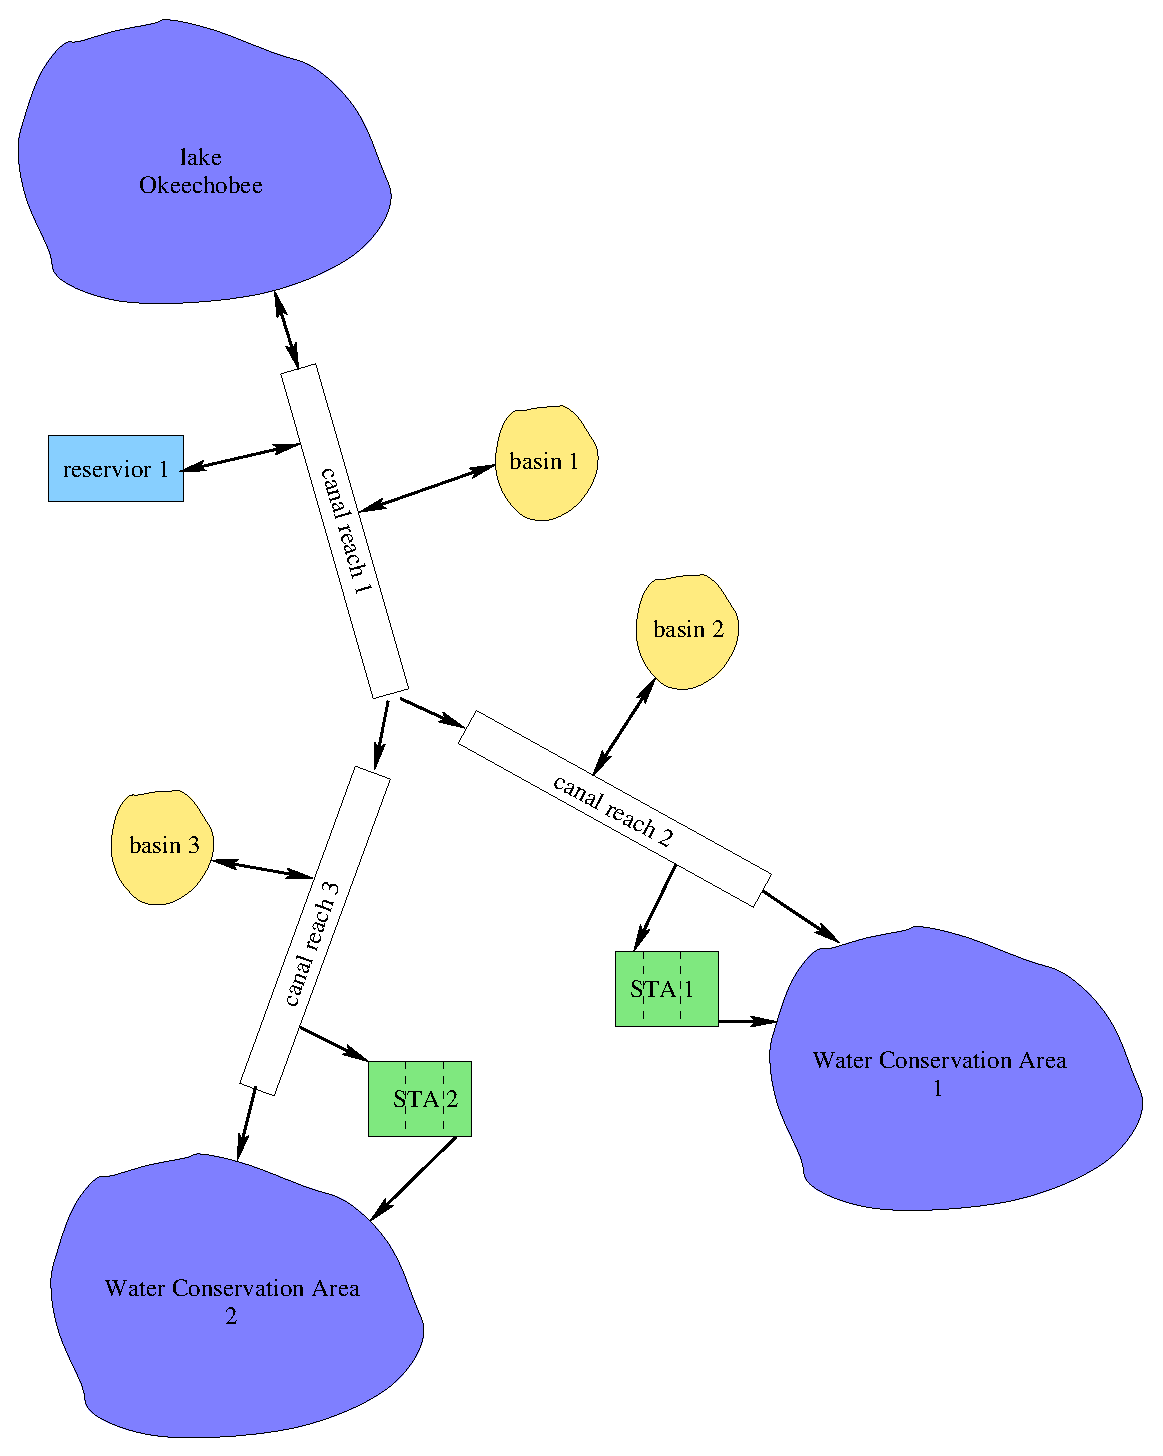
\includegraphics[scale=.5]{Graphics/eaacanal}
  \caption{\label{fig:eaacanal} EAA canal configuration}
 \end{center}
\end{figure}

The {\tt eaaCanal} assessor package is applied to each of the canal
reaches that connect an optional upstream reservoir (e.g., Lake
Okeechobee) to a downstream canal or storage area
(Figure \ref{fig:eaacanal}).  The {\tt eaaCanal} wsAssessor is
multipurpose, supervising the routing of water for:

\begin{enumerate}

 \item Flood control relief for an upstream EAA canal or reservoir;

 \item Water supply deliveries and flood control relief for adjacent
   agricultural service areas;

 \item Water supply deliveries and flood control relief for adjacent
   stormwater treatment areas;

 \item Runoff diversions to adjacent stormwater treatment areas for
   treatment;

 \item Runoff diversions to adjacent reservoirs for storage;

 \item Water supply deliveries from adjacent reservoirs; and

 \item Water supply deliveries to meet water supply needs in a
 downstream EAA canal or storage area;

\end{enumerate}

The water supply needs for the EAA canal are assessed by quantifying
the water supply requirements from adjacent service / stormwater
treatment areas and downstream outlets.  Water supply requirements are
met first by routing excess in the canal, e.g., runoff from adjacent
adjacent service / stormwater treatment areas, seepage and boundary
conditions.  Remaining water supply requirements are met by water
supply deliveries from directly connected and upstream reservoirs.

A flowchart schematic representation of the eaaCanal water supply {\tt
Assess()} function is shown in Figure \ref{fig:eaaCanalWS}.  The {\tt
eaaCanal} package for water supply has three primary operations:

 \begin{enumerate}

  \item Quantify water supply requirements from the adjacent service
  areas (SA's) and stormwater treatment areas (STA's);

  \item Quantify water supply requirements from the tailNode outlets;
  and

  \item Route local excess and compute the remaining deficit to be met
  by water supply deliveries from upstream reservoirs.

\end{enumerate}


\begin{figure}[!htb]
 \begin{center}
  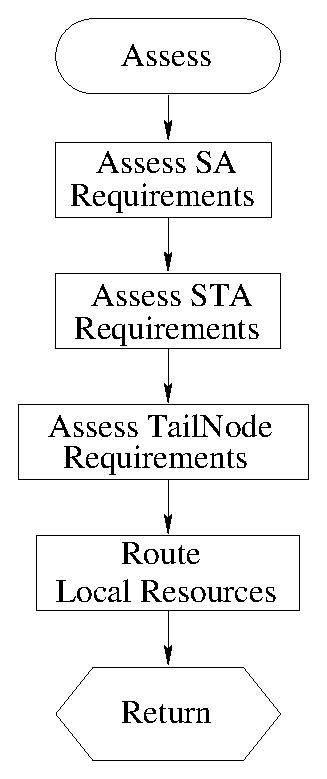
\includegraphics[scale=.5]{Graphics/eaaCanalWS}
  \caption{\label{fig:eaaCanalWS} EAA canal water supply Assess() function}
 \end{center}
\end{figure}

{\bf Compute Service / Stormwater Treatment Area Requirements}. The
water supply requirements for SA's and STA's are computed by executing
their respective water supply assessor (``wsAssessor'') functions.
Full implementation of the prioritization and allocation capabilities
in the {\tt eaaCanal} package requires a seamless integration with SA
and STA wsAssessors.  Currently, the {\tt eaaCanal} package requires
that the SA and STA wsAssessors use the {\tt std} package.  The {\tt
std} wsAssessor assesses water supply needs for the SA and STA by
computing their respective water supply requirements and distributing
the unmet water supply requirements to their water supply inlets.  The
{\tt std} package provides an option to designate the water supply
requirement with a landscape type.  For example, an agricultural WCU
would be given an ``ag'' designation.  Likewise, an environmental and
urban WCU's would be given ``env'' and ``urb'' designations,
respectively.  The {\tt eaaCanal} package uses these designations to
prioritize water supply deliveries and impose management constraints
based on landscape designation.

{\bf Compute TailNode Requirement}. A tailNode is defined as an outlet
connected to another EAA canal or a downstream storage area, such as a
Water Conservation Area.  A flowchart schematic representation for
computing the tailNode water supply requirement is shown in
Figure \ref{fig:eaaCanalWSTailNodes}.  The water supply assessor for
the downstream EAA canal is executed to quantify the water supply
requirement assigned to the tailNode.  Water supply requirement for a
downstream storage area is specified using a minimum flow constraint
for the tailNode.

\begin{figure}[!htb]
 \begin{center}
  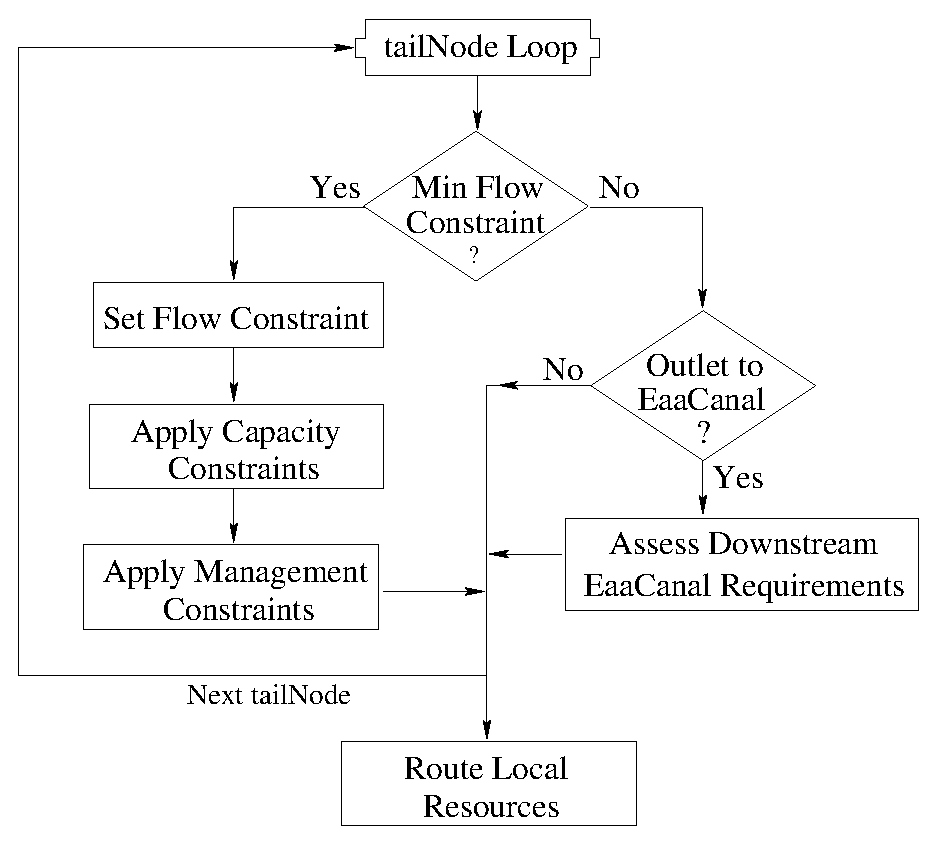
\includegraphics[scale=.5]{Graphics/eaaCanalWSTailNodes}
  \caption{\label{fig:eaaCanalWSTailNodes} EAA canal water supply tailNode assessment}
 \end{center}
\end{figure}

{\bf Route Local Resources}.  The {\tt eaaCanal} package uses the {\tt
RouteLocalResources()} function to quantify the portion of EAA canal
water supply requirement that can be met using local resources, such
as basin runoff and locally connected reservoirs.  The remaining water
supply requirements are met by regional deliveries through the
headNodes.

A schematic flowchart for the {\tt RouteLocalResources()} function is
presented in Figure \ref {fig:eaaCanalWSRouteLocal}.  The local and
regional deliveries required to meet the EAA canal water supply
requirements are assessed by following procedure:

\begin{enumerate}

  \item {\bf Estimate canal excess}.  Canal excess is defined as the
  net inflow from boundary conditions, groundwater seepage
  watermovers and estimated runoff from upstream SA's and STA's.
  Maintenance demand is defined as the inflow required to offset a
  computed negative excess.  Runoff from SA and STA WCU's is
  estimated by executing their respective fcAssessors and summing the
  resulting flood control releases through outlets discharging into
  the EAA canal.  The user can optionally restrict the use of SA or
  STA runoff for water supply.

  \item {\bf Route canal excess}.  Canal excess is routed to meet the
  water supply requirements at the canal outlets.  The water supply
  requirements are quantified by landscape type at each canal outlet.
  Canal excess is routed in ``landscape'' order, where the highest
  priority landscape types are processed first and the canal outlets are
  prioritized by downstream function: (1) outlets to stormwater
  treatment areas; (2) outlets to service areas; and (3) tailNode
  outlets.  Multiple outlets with the same function are processed in
  the order dictated by the keyword suffix specification.

  \item {\bf Route reservoir supply}.  Available supply from reservoirs
  directly connected to the canal is routed to meet the remaining
  water supply requirements at the canal outlets.  Available supply is
  routed to the water supply outlets in the same manner as the canal
  excess (i.e., in ``landscape'' order).  Reservoir releases are
  subject to management constraints that can be used to constrain
  releases based on landscape type.  Reservoirs with a headNode
  connection are processed through headNode deliveries.

  \item {\bf Compute canal deficit}.  The deficit for the canal is the
  summation of the remaining water supply requirements at the outlets,
  summed by landscape type.

  \item {\bf Set water supply requirements at headNodes}.  Canal
  deficits are resolved through regional deliveries at the headNodes.
  Water supply deliveries at a headNode are constrained by the
  remaining capacity of the headNode watermover, design capacity, and
  management constraints.  Canal deficits are distributed to multiple
  headNodes by: (1) priority order, or (2) defined fraction.  The
  priority order method assigns water supply requirements to the
  highest priority headNode in landscape order until all the canal
  deficits have been satisfied.  The defined fraction method
  distributes the canal deficit to the headNodes based on a user
  defined set of weights.
  
\end{enumerate}

\begin{figure}[!htb]
 \begin{center}
  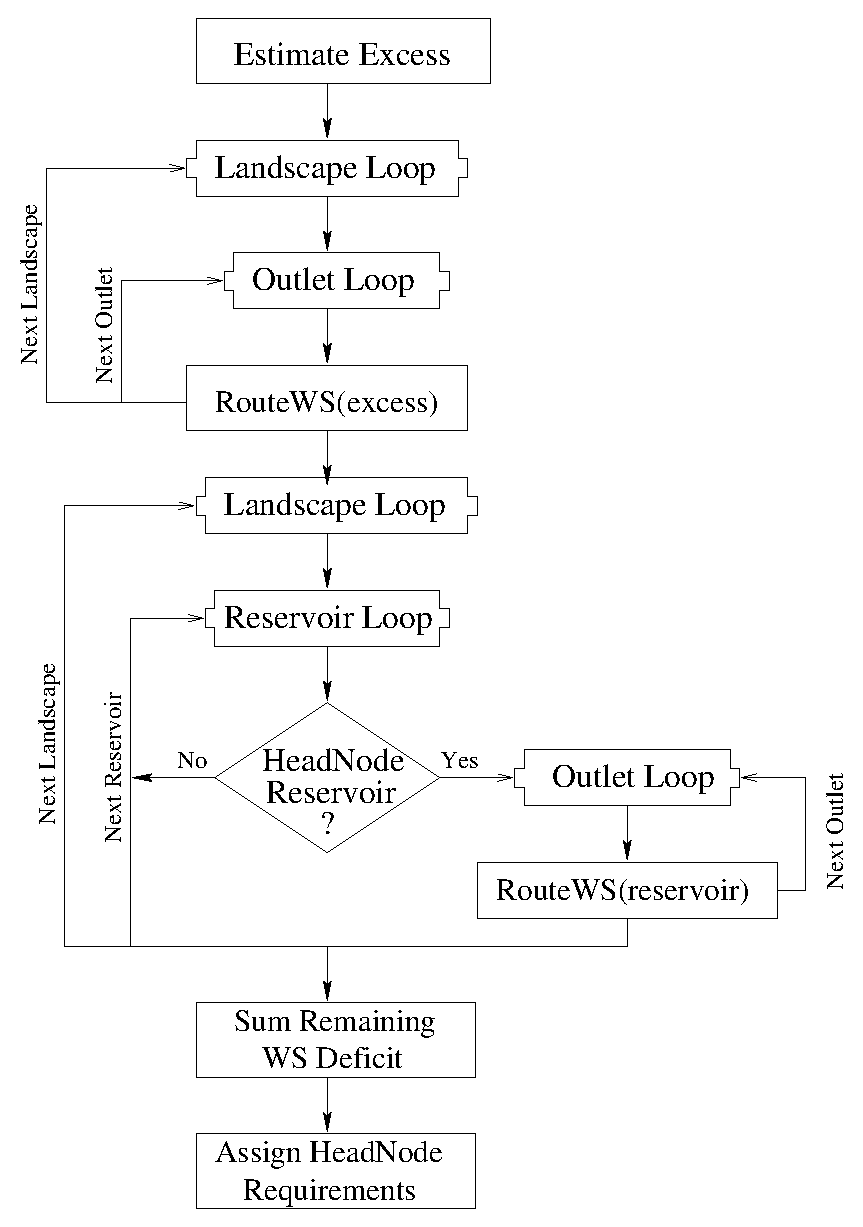
\includegraphics[scale=.5]{Graphics/eaaCanalWSRouteLocal}
  \caption{\label{fig:eaaCanalWSRouteLocal} EAA canal RouteLocalResources() schematic.}
 \end{center}
\end{figure}

The {\tt eaaCanal} prioritizes water supply releases based on the
destination's landscape type (see Table
\ref{table:eaacanalLandscape}):

\begin{table}[!htb]
 \begin{center}
  \footnotesize
  \caption{Prioritized landscape list for the {\tt eaaCanal} package. }\label{table:eaacanalLandscape}
  \begin{tabular}{p{1.0cm}p{2.0cm}p{10.0cm}}									\\[0.8ex]
   Priority	&Landscape 	&Description									\\
   \hline
   1		&maint		&inflow required to offset a computed negative excess in canal			\\
   2		&tribe		&water supply deliveries to tribal lands					\\
   2		&env		&environmental releases to maintain minimum water levels in an STA		\\
   3		&ag		&agricultural SA water supply delivery						\\
   4		&urb		&urban water supply delivery							\\
   5		&envTarg	&releases to meet target flows or water levels in environmentally sensitive areas \\
   6		&ws		&undesignated water supply delivery						\\
   \hline
  \end{tabular}
 \end{center}
\end{table}


 \subsection{{\tt estuary} package }

Water supply assessment for an estuary basin can be simulated using
the {\tt estuary} package.  Estuary water supply requirements are
imposed on its inlets using minFlow constraints.  The {\tt estuary}
package is intended to be paired with a default {\tt fcAssessor} (see
Section \ref{fcAssessor}).  By default, estuary water supply
requirements are designated as an ``envTarg'' landscape.

The {\tt estuary} package uses the following procedure to assess the
water supply needs for an estuary:

\begin{enumerate}

 \item Set the water supply requirement for each inlet,
   based on their individual minFlow constraint.

 \item Reduce water supply requirement in response to capacity and
 management constraints at each inlet.

\end{enumerate}


 \subsection{{\tt irl} package } \label{irlpackagews}

Water supply assessment in the Indian River Lagoon (IRL) basins can be
simulated using the {\tt irl} package.  The {\tt irl} package
simulates the basin interaction with a reservoir, an optional upstream
basin and a downstream estuary basin.  The {\tt irl} water supply
package is intended to be paired with a {\tt irl} assessor for flood
control (see Section \ref{irlpackagefc}).

The {\tt irl} package uses the following procedure to assess the water
supply needs for an IRL basin:

\begin{enumerate}

 \item Set basin water supply requirement to the predefined time
   series for agricultural demand and set flow for the designated
   demand outlet node.

 \item Set environmental target to the minFlow constraint placed on
   the estuary outlet.

 \item Compute basin runoff, defined as the sum of the basin boundary
   conditions flows.

 \item Compute net demand for basin (basin demand + environmental
   demand - basin runoff).

 \item Use reservoir to meet net basin demand, subject to capacity and
   management constraints, reservoir supply (volume above specified
   reserve level). Reservoir can be either multipurpose or
   agricultural only, depending on the purpose specification for the
   reservoir pump.

 \item Compute reductions to agricultural and estuary deliveries due
   to limited water supply.  Reductions are prorated, based on the
   agricultural to estuary demand ratio.

 \item Set water supply requirement for the estuary outlet and adjust
   release at the demand nodes to compensate for reductions in water
   supply delivery.

\end{enumerate}

Runoff from the optional upstream basin is not routed by the water
supply assessor.  The upstream basin runoff is added to basin excess
and routed by the {\tt irl} assessor for flood control.  


 \subsection{{\tt losa} package }

Water supply assessments for an agricultural basin in the Lake
Okeechobee Service Area (LOSA) can be simulated using the {\tt losa}
packages.  The {\tt losa} package uses following procedures to manage
a LOSA basin for water supply:

\begin{enumerate}

 \item Set basin water supply requirement to predefined time series
  for agricultural demand and set flow for the designated demand
  outlet node.  By default, the water supply requirement is designated
  as an ``ag'' landscape.

 \item Sum basin boundary condition flows.

 \item Compute regional water supply requirement (basin demand -
   boundary flows), subject to management and conveyance constraints
   and available storage in the lake.

 \item Reduce water supply release on demand outlet node if demand
   exceeds available supply.

\end{enumerate}


 \subsection{{\tt losaenv} package }\label{losaenvWS}

Water supply assessment in the Lake Okeechobee Service Area (LOSA)
basin that is upstream of an estuary basin can be simulated using the
{\tt losaenv} package.  These basins have agricultural water supply
requirement and are not connected to an upstream source, i.e., they do
NOT have a direct connection to Lake Okeechobee.  Runoff from the
basin can be used to meet environmental demand in the downstream
estuary.  This water supply assessor is intended to be paired with a
{\tt losaenv} assessor for flood control (see
Section \ref{losaenvFC}).

The {\tt losaenv} package uses the following procedure to manage a
basin for water supply:

\begin{enumerate}

 \item Set basin water supply requirement to predefined time series
 for agricultural demand and set flow for the designated demand outlet
 node.  By default this water supply requirement is designated as an
 ``ag'' landscape.

 \item Set environmental water supply requirement using the minFlow
 constraint placed on the estuary outlet.  By default this water
 supply requirement is designated as an ``envTarg'' landscape.

 \item Compute basin runoff, defined as the sum of the basin boundary
   conditions flows.

 \item Compute net demand for basin (basin demand + environmental
 demand - basin runoff).

 \item Compute reductions to agricultural and estuary deliveries due
   to limited water supply (i.e., not enough runoff).  Reductions are
   prorated, based on the agricultural to estuary demand ratio.

 \item Set water supply requirement for the estuary outlet and adjust
   release at the demand nodes to compensate for insufficient water
   supply delivery.

\end{enumerate}


 \subsection{{\tt std} package}

Standard water supply assessment for lakes and basins can be
simulated using the {\tt std} package.  The standard assessor can be
used to simulate the water supply needs for a variety of landscapes,
using different management options.  

The {\tt std} package uses the following procedures to compute water
supply requirement for the lake or basin and quantify the unmet water
supply requirements to be met by regional deliveries through the
inlets:

\begin{enumerate}
 \item Compute local water supply requirement.  The default method
   defines water supply requirement as the inflow needed to raise the
   water level up to the specified maintenance level.  This includes
   net contribution from the HPM.  The local water supply requirement
   can also be based on a preprocessed time series using the {\tt
   -predef} package modifier (e.g. {\tt package="std-predef"}).

 \item Sum boundary condition flows, outflow from unmanaged outlets,
   and inflow from unmanaged inlets.

 \item Compute unmet water supply requirement.

 \item Compute optional environmental inflow target \-- Inflow targets
   are typically defined for Stormwater Treatment Areas (STA's) and
   are designated as deliveries to an ``envTarg'' landscape.  The
   following options are available to compute the inflow target:

   \begin{enumerate}

    \item {\tt flow} - The user defines an outlet flow time series
      target for the STA outlet.  The inflow time target is the sum of
      the outlet time series plus the flow required to ``prime'' the
      STA, i.e., the volume of inflow needed to raise water level up
      to the {\tt fcLevel}.

    \item {\tt stage} - The inflow target is the inflow required to
      raise the water level up to the STA's {\tt fullLevel}.
   \end{enumerate}

 \item Set regional water supply requirements by distributing the
   unmet water supply demands to the water supply inlets. The
   following {\tt demandDist} options are available:

   \begin{enumerate}

   \item {\tt equal} - distributes unmet water supply requirement to
     the water supply inlets based on their relative available
     conveyance capacity.

   \item {\tt retReplace} - unmet water supply requirement is limited
     to the net reference evapotranspiration computed by the HPM.
     Unmet water supply requirement is distributed to the water supply
     inlets based on their relative available capacity or by the {\tt
     wsWeight} factor specified for the respective water supply
     inlets.
     
   \end{enumerate}
\end{enumerate}

A package modifier is used to designate the landscape type for the
computed water supply delivery.  This becomes important when the water
supply distribution from upstream sources is prioritized based on
landscape type.  A package modifier is formed by inserting a
recognized landscape type after {\tt std-} in the package
specification.  The water supply deliveries are recognized for the
following landscape types:

\begin{itemize}

  \item {\tt std-ag} \-- agricultural areas (default).

  \item {\tt std-env} \-- maintenance flows to environmentally
    sensitive lands (e.g., stormwater treatment areas, water
    conservation areas, wildlife management areas, etc).

  \item {\tt std-urban} \-- high to low density urban areas.

  \item {\tt std-tribe} \-- tribal lands.

  \item {\tt std-envTarg} \-- target flows to environmentally sensitive
  areas (e.g. estuaries).

\end{itemize}


 \section{Flood Control Assessors}\label{fcAssessor}

The flood control assessor quantifies the volume of excess in the
water control unit (WCU) and coordinates releases through managed
outlet structures to meet the WCU's needs as well as the regional
water supply and flood control requirements from upstream / downstream
WCU.  The {\tt default} flood control assessor package uses the
following procedure to assess WCU needs and coordinate its outlet
structure releases:

\begin{enumerate}
 \item Compute surplus flow for the water control unit.  Surplus flow
   is defined as the net inflow from WCU inlets, boundary conditions,
   unmanaged outlets, and water supply deliveries through WCU outlets.

 \item Compute stress from the WCU's hydrologic process module (HPM).

 \item Compute projected WCU storage, based on surplus flow and HPM
   stress.

 \item Compute WCU excess, defined as the volume of projected storage
   above the WCU's flood control level

 \item Set outlet releases to remove WCU excess and deliver water
   supply to meet downstream WCU needs.  Two options are available for
   distributing excess to multiple flood control outlets:

  \begin{enumerate}

    \item capacityweighted \-- distribution is weighted, based on the
      relative flood control capacity of the outlets.

    \item priorityorder \-- distribution is based on priority order
      assigned to the respective flood control outlets.

  \end{enumerate}

 \item Refine outlet releases.  Tests the downstream impact of the
   computed outlet flood control release. The degree to which
   downstream impacts are tested is controlled by the water control
   unit's fcRecursionLevel:

  \begin{enumerate}

     \item level 0 \-- do not check any downstream water control units
     \item level 1 \-- only check the flood control assessor
      immediately downstream of the water control unit
     \item level 2 \-- recursively check flood control assessors in
      downstream water control units
  \end{enumerate}
\end{enumerate}

Flood control releases at the outlet structures are limited by
capacity and management conveyance constraints.  If the downstream
water control unit is a lake with a specified fullLevel, the flood
control release is further constrained by the downstream storage
capacity.

The {\tt default} package's refine outlet flood control procedure
works by executing downstream flood control assessors as dictated by
the fcRecursionLevel and applying conveyance test to their respective
flood control outlets.  If the test fails, the flood control release
is reduced by 10\% and the downstream flood control assessor(s) are
re-executed.  This cycle of downstream flood control assessment, test,
and release reduction is repeated until the conveyance test passes or
the flood control release is reduced to zero.  The conveyance test is
specified as an {\tt dsConveyTest} for the downstream flood control
assessor (see Table \ref{WBodyFCProp}).  The following conveyance
tests are available:

\begin{enumerate}
 \item HeadTailTest \-- the estimated tail water head is compared with
   tail water head limit specified in MSE Network.  If estimated tail
   water head is higher, the test fails.

 \item LocRunoffLim \-- flood control release is limited by the local
   runoff in the downstream WCU.  Flood control release is adjusted,
   and test always passes.

 \item CapacityTest \-- flood control release is compared to the flood
   control capacity based on estimated head water and tail water heads
   at the outlet.  If release exceeds test capacity, test fails.

 \item NoFCInletRule \-- no test is applied.  Test always passes.

\end{enumerate}

The default flood control assessor methods can be overloaded by
specifying the {\tt package} attribute and specifying additional
parameters through nested elements (if needed).  Flood control
packages for WCU assessors are described and their input
specifications are defined in the following subsections.


 \subsection{{\tt eaaCanal} package} \label{fceaacanal}

The {\tt eaaCanal} flood control assessor quantifies the volume of
excess in an EAA canal and reconciles the canal's flood control needs
with regional water supply requirements at each outlet structure. The
{\tt eaaCanal} flood control assessor routes excess flow to its outlet
structures in response to the following objectives (from highest to
lowest priority): (1) use excess flow to meet local and downstream
water supply demand; (2) store excess flow in reservoirs; (3) treat
excess flow in Stormwater Treatment Areas; and (4) release untreated
excess flow through the tailNode outlet structures.

A flowchart schematic representation of the eaaCanal flood control
{\tt Assess()} function is shown in Figure \ref{fig:eaaCanalFC}. 

\begin{figure}[!htb]
 \begin{center}
  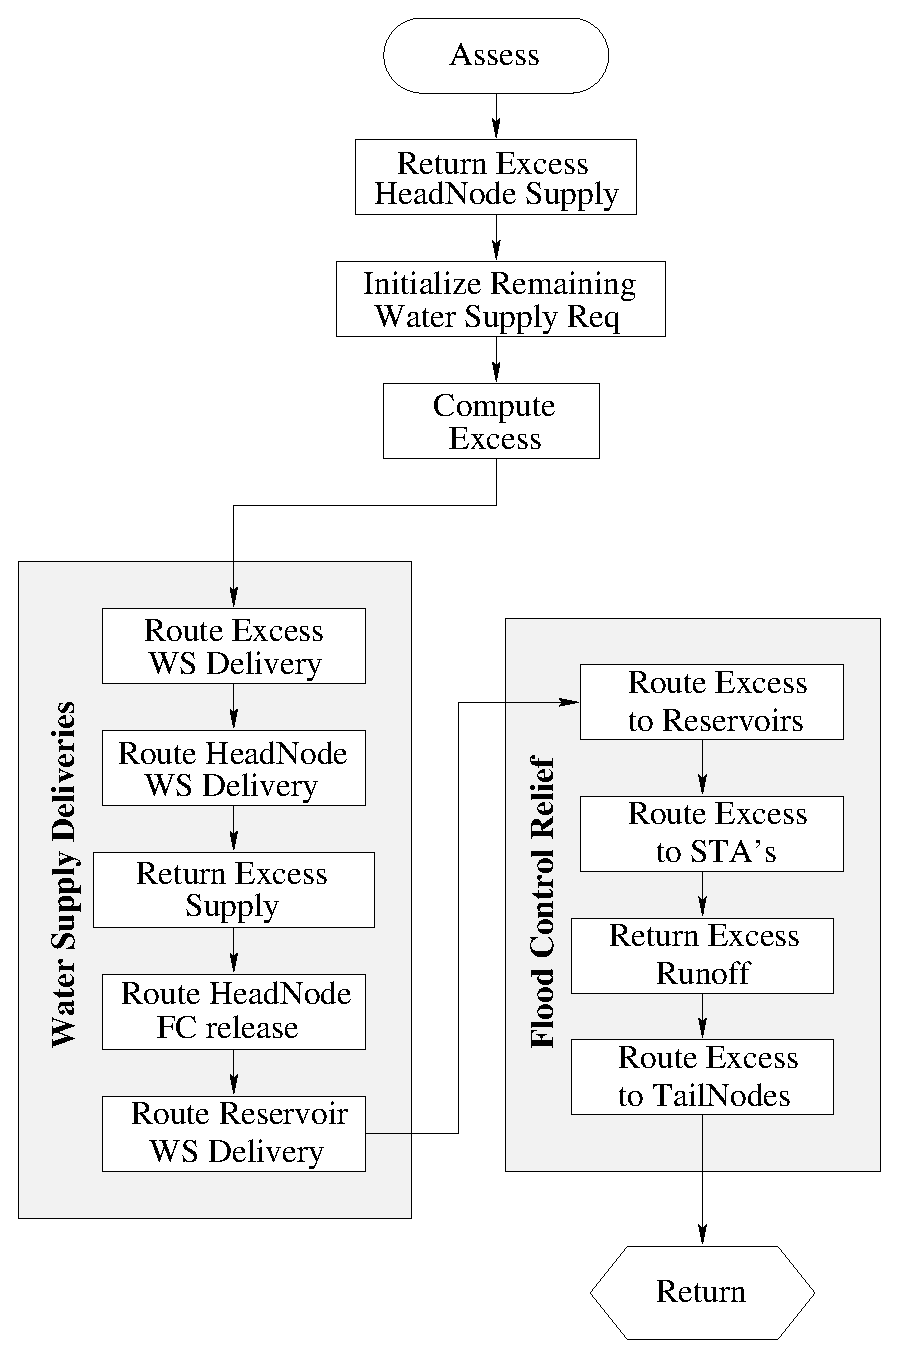
\includegraphics[scale=.5]{Graphics/eaaCanalFC}
  \caption{\label{fig:eaaCanalFC} EAA canal flood control Assess() function}
 \end{center}
\end{figure}

The {\tt eaaCanal} package uses the following procedures to address
the water supply and flood control needs for an EAA canal:

\begin{enumerate}

 \item Return excess headNode supply.  Excess water supply deliveries
   can occur when an EAA canal has multiple headNodes, and a water
   supply delivery from one headNode can be offset by a flood control
   release from another.  The excess supply is quantified and returned
   to the upstream source.

 \item Initialize remaining water supply requirement for each EAA
   canal outlet, using water supply requirements computed by the EAA
   canal's water supply assessor (see Section \ref{wseaacanal}).

 \item Compute EAA canal excess flow.  Excess volume is defined as the
   portion of projected EAA canal storage that exceeds the flood
   control level for the EAA canal.  The projected canal storage
   includes terms for boundary conditions, seepage, runoff from
   adjacent service areas and stormwater treatment areas, reservoir
   overflow, inlet flow through head nodes, and HPM stress.

 \item Route water supply deliveries.  Sources for water supply
   include canal excess flow, headNodes (water supply deliveries
   and/or flood control releases), and local reservoirs.  Water supply
   deliveries are routed in priority order based on landscape type
   (see Table \ref{table:eaacanalLandscape}).  Water supply outlets
   are processed in priority based on downstream function: (1) outlets
   to stormwater treatment areas; (2) outlets to service areas; and
   (3) tailNode outlets.  Multiple outlets with the same function are
   processed in the order dictated by the keyword suffix
   specification.

 \item Route remaining excess to adjacent reservoirs and stormwater
   treatment areas.  The flood control releases are subject to
   downstream storage availability, outlet conveyance and management
   constraints.  

 \item Route remaining canal excess flow is to tailNode outlets. If
   the remaining canal excess flow exceeds the conveyance capacity of the
   tailNode outlets, the overage is returned to their respective
   sources in the following order: 

   \begin{enumerate} 

     \item Water control units upstream of the head nodes.

     \item Directly connected stormwater treatment areas (weighted by
       their respective contributions).

     \item Directly connected agricultural service areas (weighted by
       their respective contributions).

   \end{enumerate}

   The remaining excess is distributed to multiple outlet based on
   priority order or {\tt fcWeight}.

\end{enumerate}

\textbf{\underline{Known Limitations}.} 

\begin{enumerate}
  \item Only priority order outlet distribution to the STA's and
  storage reservoirs are supported at this time.  Other distribution
  options can be added as needed.
\end{enumerate}

 \subsection{{\tt irl} package} \label{irlpackagefc}

Flood control assessment for an Indian River Lagoon (IRL) Basin can be
simulated using the {\tt irl} package. The {\tt irl} package manages
interactions between the basin and a multipurpose reservoir, optional
inlet STA, and an optional alternative outlet structure.  This flood
control assessor is intended to be paired with a {\tt irl} assessor
for water supply (see Section \ref{irlpackagews}).

The {\tt irl} package uses the following procedure to assess the flood
control needs in an IRL basin:

\begin{enumerate}

 \item Compute excess volume, defined as the portion of storage above
   the WCU's fcLevel.

 \item Compute deficit volume, defined as the portion of storage below
   the WCU's maintLevel.

 \item Compute excess flow in the basin using the following terms:
   excess and deficit volumes; basin runoff (defined as the sum of WCU
   boundary condition flows); flood control release from optional STA;
   and environmental demand release to downstream estuary;

 \item Redirect excess flow to offset environmental deficit to the
   estuary.

 \item Redirect excess flow to offset water supply releases from reservoir.

 \item Route remaining excess flow to the reservoir, subject to
   capacity, management and storage constraints.

 \item Route remaining excess flow to optional alternative outlet,
   subject to capacity and management constraints.

 \item Route remaining excess to the estuary, subject to capacity and
   management constraints.

\end{enumerate}


 \subsection{{\tt lkissQTW} package }

Flood control assessment for the combined BC Pool in the Kissimmee
River can be simulated using the {\tt lkissQTW} package.  Pool BC is
simulated as single level pool, when in reality, the restored
Kissimmee River meanders and water level changes significantly from
north to south, especially during high flow events.  The headwater
level in Pool BC (i.e., the tailwater head for the inlet structure) is
approximated using a flow versus structure tailwater head lookup
table.  This approximation is needed to provide more realistic
tailwater head estimate for the inlet capacity and gate opening
criteria computations.

The flood control needs in the {\tt lkissQTW} package are assessed
using the methods developed for the {\tt default} fcAsesessor:

\begin{enumerate}
 \item Compute surplus flow in the WCU.  This includes inflows from
   inlet nodes and boundary conditions and outflows from unmanaged and
   water supply releases from outlet nodes.

 \item Compute HPM stress from the WCU's hydrologic process module.

 \item Use surplus flow and HPM stress to compute projected WCU
   storage.

 \item Compute excess volume in the WCU, defined as the portion of
   projected storage above the WCU's flood control level

 \item Set outlet flood control releases.  The {\tt lkissQTW} package
   uses the same release methods, with the same options, as the {\tt
   default} fcAssessor package.

 \item Refine outlet flood control releases.  The {\tt lkissQTW}
   package uses the same refine methods, with the same options, as the
   {\tt default} fcAssessor package.  However, the water level at the
   upstream end of the WCU is updated using the flow versus inlet
   tailwater head lookup table.

\end{enumerate}


 \subsection{{\tt losaenv} package }\label{losaenvFC}

Flood control assessment for a Lake Okeechobee Service Area (LOSA)
basin upstream of an estuary can be simulated using the {\tt losaenv}
package. This flood control assessor is intended to be paired with a
{\tt losaenv} assessor for water supply (see Section
\ref{losaenvWS}).

The {\tt losaenv} package uses the following procedure to assess the
flood control needs in a LOSA basin:

\begin{enumerate}

 \item Compute excess volume, defined as the portion of storage
   above the WCU's fcLevel.

 \item Compute deficit volume, defined as the portion of storage below
   the WCU's maintLevel.

 \item Compute excess flow using the following terms: excess and
   deficit volumes; basin runoff (defined as the sum of the WCU
   boundary conditions flows); environmental demand release to
   downstream estuary.

 \item Route environmental and flood control releases through estuary
   outlet structure, subject to capacity and management constraints.

\end{enumerate}


 \subsection{{\tt s4Runoff} package }

Flood control assessment for the S4 drainage basin (near Lake
Okeechobee) can be simulated using the {\tt s4Runoff} package. 

The {\tt s4Runoff} package uses the following procedure to assess the
flood control needs in the S4 basin:

\begin{enumerate}

 \item Compute surplus flow in the WCU.  This includes inflows from
   inlet nodes and boundary conditions and outflows from unmanaged and
   water supply releases from outlet nodes.

 \item Retrieve water supply delivery computed for the outlet from
   Lake Okeechobee.

 \item Compute HPM stress from the WCU's hydrologic process module.

 \item Use surplus flow, water supply delivery and HPM stress to
   compute projected WCU storage.

 \item Compute excess volume in the WCU, defined as the portion of
   projected storage above the WCU's flood control level

 \item Set outlet flood control releases.  If the water level in Lake
   Okeechobee is below the backpump threshold, backpump to excess to
   the Lake, subject to conveyance and management constraints (release
   to Caloosahatchee basin is zero).  Otherwise, route a specified
   fraction of the excess to the Caloosahatchee basin, subject to
   conveyance and management constraints (the remaining balance is
   backpumped to the Lake, subject to conveyance and management
   constraints).

 \item Update water supply demand node.

\end{enumerate}


 \subsection{{\tt std} package}\label{fcassessor:std}

Standard flood control assessment for lakes and basins can be
simulated using the {\tt std} package.  The standard assessor can be
used to simulate the water supply needs for a variety of landscapes,
using different management options.  

The {\tt std} package uses the following procedure to compute excess
flow in the WCU, allocate water supply releases to water supply
outlets and set flood control releases for the flood control outlets:

\begin{enumerate}

 \item Compute excess volume in the WCU.  Excess volume is defined as
   the portion of projected storage that exceeds the flood control
   level specified for the WCU.  The projected WCU storage includes
   flow terms from inlet structure, unmanaged outlet structures,
   boundary conditions and HPM stressors.

 \item Apply optional lag fraction based on excess versus lag fraction
   lookup table.

 \item Route water supply releases to water supply outlets.  The water
   supply allocation is based on the ratio of available supply to the
   total water supply requirement.  Available water supply is defined
   as the volume of projected storage that exceeds the storage at the
   {\tt resLevel}.  If demand exceeds available supply, an allocation
   fraction is applied to all water supply releases.  

 \item Compute optional pulse flood control release.  Test the outlet
   nodes that have been designated as pulse release nodes.  If they
   are active, set pulse release to current value in the pulse release
   hydrograph, subject to conveyance limitations.  

 \item Route remaining excess flow to the flood control outlets using
   one of the following {\tt excessDist} options:

 \begin{enumerate}
  
  \item {\tt priorityOrder} (default) \-- releases to flood control
    outlet structures are computed in priority order.  Projected head
    in the WCU is updated after each flood control release, based on
    the volume that remains in storage.  The flood control release for
    each outlet is constrained by volume of remaining excess flow,
    outlet capacity (physical and design), flood control management
    constraints and available storage downstream.

  \item {\tt fcWeight} \-- excess flow is apportioned to flood control
    outlets based on a specified weighting factor.  The flood control
    release for each outlet is constrained outlet capacity (physical
    and design), flood control management constraints and available
    storage downstream.

  \item {\tt fcWeightDRE} \-- excess flow is apportioned to flood control
    outlets based on a specified weighting factor.  The flood control
    release for each outlet is constrained outlet capacity (physical
    and design), flood control management constraints and available
    storage downstream.  If there is remaining excess flow, it is
    distributed to the outlets, based on their remaining capacity.

  \item {\tt rungeKutta} \-- The Runge\--Kutta approximation method is
    used to compute flood control releases from head dependent outlet
    structures.  

  \item {\tt dsArea} - excess flow is apportioned to flood control outlets
    based on the area of the receiving water body.  The flood control
    release for each outlet is constrained outlet capacity (physical
    and design), flood control management constraints and available
    storage downstream.

  \item {\tt capacityWeighted} \-- excess flow is apportioned to flood
    control outlets using on a weighting factor based on the relative
    capacity of the flood control outlets.  The flood control release
    for each outlet is constrained outlet capacity (physical and
    design), flood control management constraints and available
    storage downstream.

 \end{enumerate}

\end{enumerate}

The standard assessor for flood control simulates a number of
management options.  Selected outlets can be designated as pulse
release nodes by using the {\tt -pulse} package modifier.  Runoff
removal rates from the WCU can be controlled using the {\tt -lag} or
{\tt -lagdepth} package modifier (e.g. {\tt package="std-pulse"}, {\tt
  package="std-lag"}).

\textbf{\underline{Known Limitations}.}  

\begin {enumerate} 

 \item Does not support the recursive checking for downstream
 conveyance constraints as computed by the {\tt default}'s
 RefineOutletQFC() method.

 \item The {\tt std} flood control and water supply assessors can not
 be guaranteed to work with other assessor packages or types because
 other water supply assessors may set their inlet flows and other
 flood control assessors generally do not assume responsibility for
 setting outlet water supply releases.  For now, the {\tt std}
 assessors are designed to work with each other as well as the {\tt
 eaaCanal} assessors.

\end{enumerate}



 \subsection{{\tt ukiss} package }

Flood control assessment for Lake Cypress and Hatchineha in the Upper
Kissimmee Chain of Lakes can be simulated using the {\tt ukiss}
package.  Since the outlet from both these lakes is uncontrolled, the
{\tt ukiss} package includes a volume check that limits the flood
control release to the volume of water that would lower its lake level
to the downstream lake level.

The flood control needs in the {\tt ukiss} package are assessed
through the following steps:
\begin{enumerate}
 \item Compute surplus flow in the WCU.  This includes inflows from
   inlet nodes and boundary conditions and outflows from unmanaged and
   water supply releases from outlet nodes.

 \item Compute HPM stress from the WCU's hydrologic process module.

 \item Use surplus flow and HPM stress to compute projected WCU
   storage.

 \item Set flood control level to the maximum outlet tailwater level.

 \item Compute excess in the WCU, defined as the volume of projected
   storage above the flood control level

 \item Set outlet flood control releases The {\tt ukiss} package
   uses the same release methods, with the same options, as the {\tt
   default} fcAssessor package.

 \item Refine outlet flood control releases The {\tt lkissQTW} package
   uses the same refine methods, with the same options, as the {\tt
   default} fcAssessor package.  

\end{enumerate}



% \section{LP Supervisors}

The runLP implementation uses a hybrid approach to manage the regional
system. North of Lake Okeechobee, an assessor coordinator routes water
through the Upper Chain of Lakes, Kissimmee, Caloosahatchee and St
Lucie river basins.  South of Lake Okeechobee, an LP supervisor routes
water through the canal network in the EAA.  The LP supervisor uses a
linear program (LP) solver to find an optimal set of structure
releases that meets water supply and flood control needs in the EAA,
subject to a series of basin storage and structure flow constraints.

The {\tt <glpk\_supervise>} element contains the specifications
required to build an independent LP model for the structures
supervised by LP.  The attributes used specify administrative details
such as the name of the LP model, input filenames, data formats, and
optimization options are listed in Table \ref {attrdefs}.

\begin{table}[!htb]
 \begin{center}
  \footnotesize
  \caption{Parameter definitions for {\tt glpk\_supervise} supervisor. }\label{attrdefs}
  \begin{tabular}{p{2.0cm}p{5.0cm}p{4.0cm}}                            \\[0.8ex]
   attribute  & Definition                    & typical value          \\
   \hline
   label      & management label              & "LP\_supervise"        \\
   modelName  & alternative label             &  "rsmbnLP"             \\ 
   modelFile  & model definition filename     & "input/mse/lp/lp.mod"  \\
   dataFile   & data specification filename   & "input/mse/lp/lp.dat"  \\
   dataFormat & data specification format     & "tabbed"               \\
   probFile   & optional output filename      & "none"                 \\
   solnFile   & optional solution filename    & "none"                 \\ 
   outputFile & optional output filename      & "none"                 \\
   method     & optimization procedure method & "simplex"              \\
   optimize   & optimization method           & "minimize"             \\
   presolve   & presolve option               & "off"                  \\
   msglevel   & message level                 & "1"                    \\
   timelimit  & time limit                    & "60"                   \\
   outfreq    & output frequency              & "1E6"                  \\
   days       & days                          & "0"                    \\ 
   hours      & hours                         & "0"                    \\
   minutes    & minutes                       & "0"                    \\
   \hline
  \end{tabular}
 \end{center}
\end{table}
\normalsize

The {\tt <glpk\_supervise>} element also defines the elements that
exchange data between the LP supervisor and the RSM.  The {\tt
  <varOut>} element takes the optimal structure flow computed by the
LP supervisor and assigns it to the corresponding watermover in the
RSM.  The {\tt <varIn>} element takes a state variable data from the
RSM and assigns it to selected parameters in the LP supervisor.

The LP model is defined in the file referenced by the modelFile
attribute.  This file contains definitions for:
\begin{enumerate}
 
 \item BASIN and STRUCTURE sets \-- collections of basin and structure
   members in the LP that are counterparts to respective waterbodies and
   watermovers in the RSM;

 \item general parameters \-- defines time step and unit conversions;

 \item basin and structure parameters \-- terms whose value is
   specified by RSM state variables through {\tt <varIn>} elements;
   and

 \item basin and structure decision variables \-- terms whose value
   is computed by the LP solver.

\end{enumerate}

The parameter and decision variable terms are used to form the linear
equations that define the objective function and a set of model
constraints.  These linear equations are defined in the file
referenced by the {\tt modelFile} attribute.

Each member of the BASIN set has the following time variant
parameters:

\begin{enumerate}
 
 \item storageInit \-- beginning of time step storage in the basin.

 \item basintarget1 \-- basin storage target \#1.  Basin storage
   deviations above and below target \# 1 storage are minimized.  Used
   to push basin water levels up or down towards a target.

 \item basintarget2 \-- basin storage target \#2.  Basin storage
   deviations below target \# 2 are minimized.  Used to maintain
   minimum water levels in the basin.

 \item basintarget3 \-- basin storage target \#3.  Basin storage
   deviations above target \# 3 are minimized.  Used to set the upper
   limit of basin storage capacity.

 \item wsDemand \-- water supply demand.  Water supply delivery
   deviations from the demand target are minimized.

 \item runoff \-- basin runoff.  Defines the boundary flow to each
   basin.

\end{enumerate}

The initial state of each basin in the BASIN set is established in the
LP model by initial storage, water supply demand and boundary flow.
Water levels in the basin are ``pushed'' up or down to minimize
deviations from specified storage targets. The LP supervisor pushes
basin water levels up or down by coordinating releases through the
basin's inlet and outlet structures.  Structure flow is limited by
physical and design capacities, and regional management objectives
expressed through constraints.

The deviations associated with each of the basin parameter targets are
weighted to reflect the priority of the respective target in the
objective function.  The following weights are static and are
specified for each member of the BASIN set:

\begin{enumerate}
 
 \item w\_target1Deficit \-- basin storage deviation below target \#1.

 \item w\_target1Excess \-- basin storage deviation above target \#1.

 \item w\_target2Deficit \-- basin storage deviations below target \#2.

 \item w\_target3Excess \-- basin storage deviations above target \#3.

 \item w\_demandDeficit \-- water supply delivery deviations from the
   demand target.

\end{enumerate}

Each member of the STRUCTURE set is defined by its upstream and
downstream basin and the following time variant parameters:

\begin{enumerate}
 
 \item maxFlow \-- maximum flow capacity of the structure.

 \item minflow \-- minimum flow target.  Deviations from this target
   are minimized.

 \item manCon \-- management constraint.  Sets the upper limit of
   allowable flow through the structure.

\end{enumerate}

Deviations from the minimum flow target are weighted globally for all
structures by single w\_minFlowDev parameter.  Each structure in the
STRUCTURE set is further defined by the following static parameters:
 
\begin{enumerate}
 
 \item name \-- structure name (usually the label of the corresponding watermover).

 \item designCap \-- structure design capacity.

 \item useManCon \-- switch that controls if the optional managed
   constraint parameter (manCon) is used.

 \item w\_flow \-- structure flow weight.  Used to penalize flow
   through selected structures.

\end{enumerate}


\subsection{Objective Function} \label{objectiveFunction}

The LP ``solves'' by minimizing its objective function, subject to
model constraints.  The objective function includes flow and deviation
terms for all the basin and structure members in the BASIN and
STRUCTURE sets:

\begin{equation}
 \begin{split}
  & \textrm { minimize objective } : \\
  & \textrm { sum \{ i in BASIN \} (}   \\
  & \quad \textrm { w\_target1Excess [i] * target1Excess [i] } + \\
  & \quad \textrm { w\_target1Deficit [i] * target1Deficit [i] } +  \\
  & \quad \textrm { w\_target2Deficit [i] * target2Deficit [i] } + \\
  & \quad \textrm { w\_demandDeficit [i]  * demandDeficit [i] } + \\
  & \quad \textrm { w\_target3Excess [i]  * target3Excess [i] )} + \\
  & \textrm { sum  \{ (i,j) in STRUCTURE \} } \textrm { ( w\_flow [i,j] * flow [i,j] ) }+ \\
  & \textrm { sum  \{ (i,j) in STRUCTURE \} } \textrm { ( w\_minFlowDev * minFlowDev [i,j] ) }
 \end{split}
\end{equation}

The weight factors in the objective function static parameters defined
by the user.  The flow and target deviation terms are decision
variables that are computed by the LP solver.  These decision
variables are also used to form the linear equations that define model
constraints.

The objective function minimizes the summation of:

\begin{enumerate}
 
 \item deviations from basin storage targets, 

 \item deviations from water supply demand targets, 

 \item structure flow penalties, and

 \item deviations from structure minimum flows.

\end{enumerate}

A target or penalty term can be dropped from the objective function by
setting their corresponding weight factor to 0.0.  Likewise, the
priority of a target or penalty term can be elevated by increasing its
weight factor relative to the weight factors to assigned to other
targets and penalty terms.

\subsection{Model Constraints} 

Model constraints are linear equations that use decision variable
terms.  The following decision variables are computed by the solver
for every member of the BASIN set:

\begin{enumerate}
 
 \item storageFinal \-- end of time step basin storage 
 \item target1Excess \-- volume of basin storage in above target \#1
 \item target1Deficit \-- volume of storage below target \#1
 \item target2Deficit \-- volume of storage below target \#2
 \item target3Excess \-- volume of storage above target \#3
 \item demandDeficit \-- volume of water supply deficit
 \item wsDemandActual \-- volume of water supply delivered

\end{enumerate}

All basin decision variables are restricted to values greater than or
equal to 0.0.

The following decision variables are computed by the solver for every
member of the STRUCTURE set:

\begin{enumerate}
 
 \item flow \-- volume of flow from upstream to downstream basin
 \item minFlowDev \-- deviation from minimum flow target

The flow decision variable is defined for every member of STRUCTURE
set and is restricted to values greater than or equal to 0.0.

\end{enumerate}

Model constraints fall into several broad categories: continuity,
basin constraints, flow constraints and canal specific constraints.
Each are entered into the LP solver as linear equations comprised of
parameter and decision variables.  The following sections describe
each category in more detail.


\subsubsection{Continuity constraint}

The conservation of mass constraint includes terms for beginning of
time step basin storage (storageInit), runoff, water supply delivery
(wsDemandActual), structure inflow and outflow:

\begin{equation}
 \begin{split}
   \textrm {subject to } & MassConservation \textrm { \{ i in BASIN \}} : \\
   \textrm {storageFinal [i]} & = \textrm { storageInit [i]} \\
                   & + \textrm {runoff [i] * unitFlow} \\
                   & - \textrm {wsDemandActual [i] * unitFlow} \\
                   & + \textrm {sum \{ (j,i) in STRUCTURE \} }  \textrm {flow [j,i]} \\ 
                   & - \textrm {sum \{ (i,j) in STRUCTURE \} }  \textrm {flow [i,j]} 
 \end{split}
\end{equation}

where the values for storageInit and runoff are set by {\tt <varIn> }
elements.  The \textrm {sum \{ (j,i) in STRUCTURE \} \{flow [i,j]\}} terms
sum structure inflows and outflows for the respective basins.  The
wsDemandActual term is based on the demand deviation from water supply
demand parameter:

\begin{equation}
 \begin{split}
  \textrm { subject to } DemandDeviation  & \textrm { \{ i in BASIN \} } : \\
  \textrm { wsDemandActual [i] } & =  \textrm { wsDemand [i] - demandDeficit [i] } 
 \end{split}
\end{equation}

The demandDeficit term is minimized through its inclusion in the
objective function.  

\subsubsection {Basin Constraints }

Basin water levels are managed by minimizing deviations from storage
targets.  Target \#1 is designed to minimize deviations above and
below the target:

\begin{equation}
 \begin{split}
  \textrm { subject to } Target1Deviation  & \textrm { \{ i in BASIN \} } : \\
  \textrm { storageFinal [i] } & = \textrm { basinTarget1 [i] + target1Excess [i] - target1Deficit [i] }
 \end{split}
\end{equation} 

where the basinTarget1 parameter is set by a {\tt <varIn> } element.
The target1Excess and target1Deficit terms are both weighted and
minimized through their inclusion in the objective function.  Target
\#2 is designed to minimize deviations below the target:

\begin{equation}
 \begin{split}
  \textrm { subject to } Target2Deviation  & \textrm { \{ i in BASIN \} } : \\
  \textrm { storageFinal [i] } & \ge \textrm { basinTarget2 [i] - target2Deficit [i] }
 \end{split}
\end{equation}

where the basinTarget2 parameter is set by a {\tt <varIn> } element.
The target2Deficit term is weighted and minimized through its
inclusion in the objective function.  Target \#3 is designed to
minimize deviations above the target:

\begin{equation}
 \begin{split}
  \textrm { subject to } Target3Deviation & \textrm { \{ i in BASIN \} } : \\
  \textrm { storageFinal [i] } & \le \textrm { basinTarget3 [i] + target3Excess [i] }
 \end{split}
\end{equation}

where the basinTarget3 parameter is set by a {\tt <varIn> } element.
The target3Excess term is weighted and minimized through its inclusion
in the objective function.

\subsubsection {Flow Constraints }

Structure flow is constrained by minimum flow, maximum flow and
management constraints.  The minimum flow constraint is implemented as
a target by minimizing the deviation between minflow and flow:

\begin{equation}
 \begin{split}
  \textrm { subject to } MinimumFlow & \textrm { \{ (i,j) in STRUCTURE \} } : \\
  \textrm { minFlowDev [i,j] } & \ge  \textrm { minflow [i,j] * unitFlow - flow [i,j] } 
 \end{split}
\end{equation}

where the minflow parameter is set by a {\tt <varIn> } element.  The
minFlowDev and flow terms are minimized through their inclusion in the
objective function.  The maximum flow constraint sets an upper bound
on structure flow:

\begin{equation}
 \begin{split}
    \textrm {subject to } FlowCapacity & \textrm { \{ (i,j) in STRUCTURE \}} : \\ 
    \textrm {flow [i,j]} & \le \textrm {maxFlow [i,j] * unitFlow} 
 \end{split}
\end{equation}

where the maxFlow parameter is set by a {\tt <varIn> } element.
Managed constraints are applied only if the useManCon value for the
respective structure is set to 1.  When applied, the managed
constraint sets an upper bound on structure flow:

\begin{equation}
 \begin{split}
    \textrm {subject to } & ManagedConstraint \textrm { \{ (i,j) in STRUCTURE \} } :  \\ 
    &\textrm {if useManCon [i,j]} \\ 
    &\textrm {then flow [i,j]} \le \textrm { manCon [i,j] * unitFlow } 
 \end{split}
\end{equation}

where the manCon parameter is set by a {\tt <varIn> } element and
useManCon value is set in the static model data block for structures.

\subsubsection {Canal Specific Constraints }

The constraints applied to the members of the BASIN and STRUCTURE sets
are generically applied to all the basins and structures in their
respective sets.  Sometimes it is desirable to apply constraints to
selected basins and structures.  For example, five basins discharge
their runoff into the North New River \-- Hillsboro Canal. If the
total runoff exceeds the outlet flow capacity of the canal or the
downstream storage capacity, it is desirable to prorate the discharge
uniformly from each of the five basins.  The following template is
used as a constraint for each basin connected to the North New River
\-- Hillsboro Canal:

\begin{equation}
 \begin{split}
  \textrm { subject to } &subbasinMin: \\
  &\textrm { SubbasinMin } = \textrm {  minflow['subbasin', 'nnrHills'] * unitFlow } \\  
  \textrm { subject to } &subbasinDev: \\
  &\textrm { SubbasinMin } = \textrm { flow['subbasin', 'nnrHills'] + SubbasinExcess } \\ 
  \textrm { subject to } &subbasinExcess: \\
  &\textrm { SubbasinExcess } =\textrm {  minflow['subbasin', 'nnrHills'] * ExcessRatioNNR }
 \end{split}
\end{equation}

where the name of the basin is substituted for \textrm {'subbasin''}
and \textrm {'Subbasin''}.  The $subbasinMin$ constraint sets \textrm
{SubbasinMin} equal to the minflow for a specific structure.  The
$subbasinDev$ constraint computes the flow deviation from \textrm
{SubbasinMin} (i.e., \textrm {SubbasinExcess}).  The $subbasinExcess$
constraint requires that \textrm {SubbasinExcess} be equivalent to a
fraction of \textrm {SubbasinMin} (\textrm {ExcessRatioNNR}).  Since
\textrm {ExcessRatioNNR} is the same for all the basins connected to
the North New River \-- Hillsboro Canal, the constraints will enforce uniform
prorating for all the basin runoff.  

The following decision variables were defined for canal specific
constraints applied to the North New River \-- Hillsboro and Upper
Miami Canals:

\begin{enumerate}
 \item SSDDExcess \-- excess runoff from South Shore Drainage District
   to North New River \-- Hillsboro Canal
 \item SSDDMin \-- minimum flow from South Shore Drainage District to
   North New River \-- Hillsboro Canal
 \item ClosterExcess \-- excess runoff from Closter Farms to North New
   River \-- Hillsboro Canal
 \item ClosterMin \-- minimum flow from Closter Farms to North New River \--
   Hillsboro Canal
 \item ESWCDExcess \-- excess runoff from East Shore Water Control
   District to North New River \-- Hillsboro Canal
 \item \-- ESWCDMin \-- minimum flow from East Shore Water Control
   District to North New River \-- Hillsboro Canal
 \item S5AExcess \-- excess runoff from S5A basin to North New River
   \-- Hillsboro Canal
 \item \-- S5AMin \-- minimum flow from S5A basin to North New River
   \-- Hillsboro Canal
 \item NNRHillsExcess \-- excess runoff from North New River \-- Hillsboro
   Basin to North New River \-- Hillsboro Canal
 \item NNRHillsMin \-- minimum flow from North New River \-- Hillsboro
   Basin to North New River \-- Hillsboro Canal
 \item MiamiBasinExcess \-- excess runoff from Miami Basin to Upper
   Miami Canal
 \item MiamiBasinMin \-- minimum flow from Miami Basin to Upper Miami
   Canal
 \item SSDDMiaExcess \-- excess runoff from South Shore Drainage
   District to Upper Miami Canal
 \item SSDDMiaMin \-- minimum flow from South Shore Drainage District
   to Upper Miami Canal
 \item SFCDExcess \-- excess runoff from South Florida Conservancy
   District to Upper Miami Canal
 \item SFCDMin \-- minimum flow from South Florida Conservancy
   District to Upper Miami Canal
 \item L1EExcess \-- excess runoff from L1E Basin to Upper Miami Canal
 \item L1EMin \-- minimum flow from L1E Basin to Upper Miami Canal
 \item ExcessRatioNNR \-- excess ratio applied to basin runoff
   discharged to North New River \-- Hillsboro Canal
 \item ExcessRatioMiami \-- excess ratio applied to basin runoff
   discharged to Upper Miami Canal
\end{enumerate}


\subsection{LP Model Data}

The initial condition for each basin is established for the LP by
initial basin storage, boundary flow (runoff), water supply demand and
target storage levels \#1, \#2 and \#3.  All these parameter values
are updated daily for each basin by their respective {\tt <varIn>}
elements. By convention, each member of the BASIN set is entered into
a data block with initial parameter values for each of the respective
basins.  Likewise, each member of the STRUCTURE set is entered into a
data block with the structure's upstream and downstream basin name and
initial parameter values for each of the respective structures.  This
data structure simplifies the way parameters are updated in the RSM.
Since the values from the corresponding {\tt <varIn>} entries
overwrite the initial parameter values in the data blocks, the actual
values for the initial basin and structure parameters are disregarded.
The parameter data blocks for BASIN and STRUCTURE sets are specified
in the file referenced by the {\tt dataFile} attribute.

The list of members in the BASIN set and the source of data for each
basin parameter are presented in Table \ref{TVbasinPara}.  Possible
sources of data for basin parameter values include:

\begin{enumerate}
 
 \item wbhead \-- beginning of time step head simulated for the
   respective basin by the HSE.

 \item rulecurve \-- schedule specified in the MSE.

 \item constant \-- value specified in {\tt <varIn>} element.

 \item external \-- pre-processed times series data stored in DSS file.

 \item bcflows \-- summation of boundary condition flows computed by
   an HSE assessor.

\end{enumerate}

The maxFlow, minflow and manCon parameter values for each structure
are updated daily by their respective {\tt <varIn>} elements.  The
list of members in the STRUCTURE set and the source for each parameter
are presented in Tables \ref {strParaTs_1} and \ref {strParaTs_2}.
Possible sources for structure parameters values include:

\begin{enumerate}
 
 \item wmcap \-- maximum flow capacity computed by the HSE.

 \item assessor (FC) \-- flood control requirement computed by an {\tt
   <AssessorCoordinator> } flood control assessor.

 \item assessor (WS) \-- water supply requirement computed by an {\tt
   <AssessorCoordinator> } water supply assessor.

 \item constant \-- value specified in {\tt <varIn>} element.

 \item external \-- pre-processed times series data stored in DSS
   file.

\end{enumerate}

The LP data file is also used to specify values for static basin and
structure parameters.  The static basin parameters used to weight
deviations from basin storage and water supply targets are listed in
Table \ref {StaticbasinPara}.  The static structure parameters used to
define structure name, design capacity, optional use of manCon's and
structure flow penalty are listed in Tables \ref{strParaConst_1}
and \ref{strParaConst_2}.

\subsection {Optimization strategies}

\subsubsection {Canal}

Canals in the EAA are assumed to provide no local storage, which means
inflow must equal outflow for each time step.  This is accomplished it
the LP by by placing a high penalty (100) on deviations above and
below target \#1 storage for each canal in the EAA.  Target \#1
storage is computed by the respective {\tt <wbmonitor>}, based on a
target water level that coincides with the canal's {\tt fcLevel} and
{\tt maintLevel}.

\subsubsection {Service Area with HPM}

The hydrology for a service area basin is simulated by a hydrologic
process module (HPM) in RSM.  Assessors quantify the water supply and
flood control requirements for the basin and distribute the
requirements to the basin's inlets and outlets.  The water supply
requirement for an inlet is retrieved through a monitor ({\tt
  <qpackmonitor comp="ws" attr="req">}) and entered as a minflow and
maxFlow constraint on the corresponding structure in the LP.  Setting
minflow and maxFlow to the same value ensures that the water supply
requirement will be met (subject to capacity and supply constraints),
and the LP will not divert additional flow to the basin for storage or
as a pass through to meet downstream needs.  Likewise, the flood
control requirement for an outlet is retrieved through a monitor {\tt
  <qpackmonitor comp="ws" attr="req">} and entered as a minflow and
maxFlow constraint on the corresponding structure in the LP.  Setting
the minflow and maxFlow to the same value ensures that the flood
control flood control needs of the basin are meet, subject to capacity
and storage constraints, and the LP will not attempt to use basin
storage or use the basin as a pass through to to meet water supply
needs elsewhere.

The maxFlow constraint is entered into the LP as an inequality,
thereby guaranteeing the flow will not exceed maxFlow.  The minflow
constraint is entered as a target and the deviation from the target is
minimized.  The penalty for missing the minflow target is universally
set to 10.

\subsubsection {Service Area \-- without HPM}

The hydrology for some service area basins is simulated by other
models (e.g., SFWMM, AFSIRS\--WATBAL, etc).  The water supply and
flood control requirements for the basin's inlets and outlets are
preprocessed and retrieved through a monitor ({\tt <dssmonitor>}) and
entered as a minflow and maxFlow constraint on the corresponding
structure in the LP.  As with service areas with HPM's, minflow and
maxFlow values for the inlets and outlets are set to ensure
requirements are met and the basin is not used as a reservoir or as a
pass through facility.  Unlike basins with HPM's, water supply
delivered to the basin do not have an HPM to remove the water from
the RSM model domain.  Service areas without HPM's use on a demandNode
to remove the water supply delivery from the RSM domain.  The minflow
and maxFlow value for the demandNode is set to the same value as the
water supply requirement as the basin inlets.

by a hydrologic process module (HPM) in RSM.  Assessors quantify the
water supply and flood control requirements for the basin and
distribute the requirements to the basin's inlets and outlets.  The
water supply requirement for an inlet is retrieved through a monitor
({\tt <qpackmonitor comp="ws" attr="req">}) and entered as a minflow
and maxFlow constraint on the corresponding structure in the LP.
Setting minflow and maxFlow to the same value ensures that the water
supply requirement will be met (subject to capacity and supply
constraints), and the LP will not divert additional flow to the basin
for storage or as a pass through to meet downstream needs.  Likewise,
the flood control requirement for an outlet is retrieved through a
monitor {\tt <qpackmonitor comp="ws" attr="req">} and entered as a
minflow and maxFlow constraint on the corresponding structure in the
LP.  Setting the minflow and maxFlow to the same value ensures that
the flood control flood control needs of the basin are meet, subject
to capacity and storage constraints, and the LP will not attempt to
use basin storage or use the basin as a pass through to to meet water
supply needs elsewhere.

The maxFlow constraint is entered into the LP as an inequality,
thereby guaranteeing the flow will not exceed maxFlow.  The minflow
constraint is entered as a target and the deviation from the target is
minimized.  The penalty for missing the minflow target is universally
set to 10.


\subsubsection {Stormwater Treatment Area}
 * Canal storage is constant, i.e., inflow equals outflow for each time step.  This enforced by  


\begin{table}[!htb]
 \begin{center}
  \footnotesize
  \caption{Example of the LP time variant basin parameters. }\label{TVbasinPara}
  \begin{tabular}{p{2.3cm}p{1.8cm}p{1.8cm}p{1.8cm}p{1.8cm}p{1.8cm}p{1.8cm}}         \\[0.8ex]
   basin          &storageInit &target1   &target2   &target3   &wsDemand &runoff   \\
  \hline
  lo              &wbhead      &rulecurve &rulecurve & 1000     & 0       & 0       \\
  L8              &wbhead      & 10       & 10       & 1000     & 0       & 0       \\
  C51W            &wbhead      & 10       & 10       & 1000     & 0       & 0       \\
  C51             &wbhead      & 10       & 10       & 1000     & 0       & 0       \\
  L10L12          &wbhead      & 9.5      & 9.5      & 1000     & 0       & 0       \\
  nnrHills        &wbhead      & 8        & 8        & 1000     & 0       & 0       \\
  umiami          &wbhead      & 8.5      & 8.5      & 1000     & 0       & 0       \\
  lmiami          &wbhead      & 8        & 8        & 1000     & 0       & 0       \\
  L5E             &wbhead      & 9        & 9        & 1000     & 0       & 0       \\
  L3Canal         &wbhead      & 8        & 8        & 1000     & 0       & 0       \\
  L8basin         &wbhead      & 8        & 8        & 1000     & 0       &external \\
  C51Basin        &wbhead      & 8        & 8        & 1000     & 0       &external \\
  C51WBasin       &wbhead      & 8        & 8        & 1000     & 0       &external \\
  S5ABasin        &wbhead      & 5        & -5       & 1000     & 0       & 0       \\
  ebwcd           &wbhead      & 5        & -5       & 1000     & 0       & 0       \\
  eswcd           &wbhead      & 5        & -5       & 1000     & 0       & 0       \\
  closter         &wbhead      & 5        & -5       & 1000     & 0       & 0       \\
  ssdd            &wbhead      & 5        & -5       & 1000     & 0       & 0       \\
  sfcd            &wbhead      & 5        & -5       & 1000     & 0       & 0       \\
  NnrHillsBasin   &wbhead      & 5        & -5       & 1000     & 0       & 0       \\
  miamiBasin      &wbhead      & 5        & -5       & 1000     & 0       & 0       \\
  rotenberger     &wbhead      &rulecurve &rulecurve & 1000     & 0       &bcflows  \\
  holeyland       &wbhead      & 13       &rulecurve & 1000     & 0       &bcflows  \\
  L1EBasin        &wbhead      & 25       & 10       & 1000     & 0       & 0       \\
  L2CBasin        &wbhead      & 25       & 10       & 1000     & 0       & 0       \\
  annexBasin      &wbhead      & 25       & 10       & 1000     & 0       & 0       \\
  ussugarUnit2    &wbhead      & 25       & 10       & 1000     & 0       & 0       \\
  bigCypRes       &wbhead      & 25       & 10       & 1000     & 0       & 0       \\
  STA1InflowCanal &wbhead      & 16.5     & 16.5     & 1000     & 0       & 0       \\
  sta1e           &wbhead      & 15.565   & 14.815   & 18.315   & 0       &bcflows  \\
  sta1w           &wbhead      & 11.06428 & 10.31428 & 14.31428 & 0       &bcflows  \\
  STA2InflowCanal &wbhead      & 10       & 10       & 1000     & 0       & 0       \\
  sta2            &wbhead      & 11.41    & 10.6     & 14.6     & 0       &bcflows  \\
  sta34sc         &wbhead      & 8        & 8        & 1000     & 0       & 0       \\
  sta34           &wbhead      & 10.72    & 9.97     & 13.97    & 0       &bcflows  \\
  sta5            &wbhead      & 13.83    & 12.63    & 16.63    & 0       &bcflows  \\
  sta6            &wbhead      & 14.07    & 13.28    & 17.28    & 0       &bcflows  \\
  wca1            &wbhead      & 20       & 7        & 1000     & 0       & 0       \\
  wca2a           &wbhead      & 20       & 7        & 1000     & 0       & 0       \\
  wca3a           &wbhead      & 20       & 7        & 1000     & 0       & 0       \\
  dummyLake       &wbhead      & 0        & 0        & 1000     & 0       & 0       \\
  \hline
  \end{tabular}
 \end{center}
\end{table}
\normalsize

\begin{table}[!htb]
 \begin{center}
  \footnotesize
  \caption{Example of the LP static basin parameter values. }\label{StaticbasinPara}
  \begin{tabular}{p{2.5cm}p{2.2cm}p{2.2cm}p{2.2cm}p{2.2cm}p{2.2cm}}                  \\[0.8ex]
   basin          &w\_target1Deficit &w\_target1Excess  &w\_target3Excess &w\_target2Deficit &w\_demandDeficit \\
  \hline 
  lo              &   0         &    0          &    0         &     0         &    0 \\
  L8              & 100         &  100          &    0         &     0         &    0 \\
  C51W            & 100         &  100          &    0         &     0         &    0 \\
  C51             & 100         &  100          &    0         &     0         &    0 \\
  L10L12          & 100         &  100          &    0         &     0         &    0 \\
  nnrHills        & 100         &  100          &    0         &     0         &    0 \\
  umiami          & 100         &  100          &    0         &     0         &    0 \\
  lmiami          & 100         &  100          &    0         &     0         &    0 \\
  L5E             & 100         &  100          &    0         &     0         &    0 \\
  L3Canal         & 100         &  100          &    0         &     0         &    0 \\
  L8basin         & 100         &  100          &    0         &     0         &    0 \\
  C51Basin        & 100         &  100          &    0         &     0         &    0 \\
  C51WBasin       & 100         &  100          &    0         &     0         &    0 \\
  S5ABasin        &   0         &    0          &    0         &     0         &    0 \\
  ebwcd           &   0         &    0          &    0         &     0         &    0 \\
  eswcd           &   0         &    0          &    0         &     0         &    0 \\
  closter         &   0         &    0          &    0         &     0         &    0 \\
  ssdd            &   0         &    0          &    0         &     0         &    0 \\
  sfcd            &   0         &    0          &    0         &     0         &    0 \\
  NnrHillsBasin   &   0         &    0          &    0         &     0         &    0 \\
  miamiBasin      &   0         &    0          &    0         &     0         &    0 \\
  rotenberger     &   0         &    1          &  100         &   100         &    0 \\
  holeyland       &   0         &    1          &  100         &   100         &    0 \\
  L1EBasin        &   0         &    0          &    0         &     0         &    0 \\
  L2CBasin        &   0         &    0          &    0         &     0         &    0 \\
  annexBasin      &   0         &    0.001      &    0         &     0         &    0 \\
  ussugarUnit2    &   0         &    0.001      &    0         &     0         &    0 \\
  bigCypRes       &   0         &    0          &    0         &     0         &    0 \\
  STA1InflowCanal & 100         &  100          &    0         &     0         &    0 \\
  sta1e           &   0         &    0.001      &  100         &   100         &    0 \\
  sta1w           &   0         &    0.001      &  100         &   100         &    0 \\
  STA2InflowCanal & 100         &  100          &    0         &     0         &    0 \\
  sta2            &   0         &    0.001      &  100         &   100         &    0 \\
  sta34sc         & 100         &  100          &    0         &     0         &    0 \\
  sta34           &   0         &    0.01       &  100         &   100         &    0 \\
  sta5            &   0         &    1          &  100         &   100         &    0 \\
  sta6            &   0         &    1          &  100         &   100         &    0 \\
  wca1            &   0         &    0          &    0         &     0         &    0 \\
  wca2a           &   0         &    0          &    0         &     0         &    0 \\
  wca3a           &   0         &    0          &    0         &     0         &    0 \\
  dummyLake       &   0         &    0          &    0         &     0         &    0 \\
  \hline
  \end{tabular}
 \end{center}
\end{table}
\normalsize

\begin{table}[!htb]
 \begin{center}
  \footnotesize
  \caption{Example of the LP time varying structure parameter values (Part 1). }\label{strParaTs_1}
  \begin{tabular}{p{2.5cm}p{2.0cm}p{2.0cm}p{2.0cm}}            \\[0.8ex]
  structure        &maxFlow         &minflow          &manCon  \\
  \hline
  C10A             &wmcap           &assessor (FC)    & 100000  \\
  S352             &wmcap           &assessor (FC)    & 100000  \\
  S351             &wmcap           &assessor (FC)    & 100000  \\
  S354             &wmcap           &assessor (FC)    & 100000  \\
  C10              &assessor (WS)   &assessor (WS)    & 100000  \\
  C12              &assessor (WS)   &assessor (WS)    & 100000  \\
  C12A             &assessor (WS)   &assessor (WS)    & 100000  \\
  C4A              &assessor (WS)   &assessor (WS)    & 100000  \\
  S236             &assessor (WS)   &assessor (WS)    & 100000  \\
  S5AE             &wmcap           & 0               & 100000  \\
  L8canal2basin    &assessor (WS)   &assessor (WS)    & 100000  \\
  CWPB2            &external        &external         & 100000  \\
  S155A            &wmcap           & 0               & 100000  \\
  C51Wcanal2basin  &assessor (WS)   &assessor (WS)    & 100000  \\
  S319             &wmcap           & 0               & assessor\\
  C51canal2basin   &assessor (WS)   &assessor (WS)    & 100000  \\
  S155             &wmcap           & 0               & 100000  \\
  S5A              &wmcap           & 0               & 100000  \\
  L10L12toS5ABasin &assessor (WS)   &assessor (WS)    & 100000  \\
  S2               &wmcap           & 0               &assessor \\
  G371             &wmcap           & 0               & 100000  \\
  nnr2nnrHills     &assessor (WS)   &assessor (WS)    & 100000  \\
  S6               &wmcap           & 0               & 100000  \\
  G370             &wmcap           & 0               & 100000  \\
  S3               &wmcap           & 0               &assessor \\
  G373             &wmcap           & 0               & 100000  \\
  mc2miaBasin      &assessor (WS)   &assessor (WS)    & 100000  \\
  G372             &wmcap           & 0               & 100000  \\
  G410             &wmcap           & 0               & 100000  \\
  L4toBigCypRes    &assessor (WS)   &assessor (WS)    & 100000  \\
  G507             &wmcap           & 0               & 100000  \\
  s8               &wmcap           &external         & 100000  \\
  L4gap            &wmcap           & 0               & 100000  \\
  S7               &wmcap           &external         & 100000  \\
  S150             &wmcap           &external         & 100000  \\
  G407             &wmcap           & 0               & 100000  \\
  G353             &wmcap           & 0               & 100000  \\
  \hline                                                                            
  \end{tabular}
 \end{center}
\end{table}
\normalsize

\begin{table}[!htb]
 \begin{center}
  \footnotesize
  \caption{Example of the LP time varying structure parameter values (Part 2). }\label{strParaTs_2}
  \begin{tabular}{p{2.8cm}p{2.0cm}p{2.0cm}p{2.0cm}}                \\[0.8ex]
  structure        &maxFlow           &minflow          &manCon    \\
  \hline
  basin2L8canal    &assessor (FC)     &assessor (FC)    & 100000   \\
  L8DemandNode     &assessor (WS)     &assessor (WS)    & 100000   \\
  basin2C51Wcanal  &assessor (FC)     &assessor (FC)    & 100000   \\
  C51WDemandNode   &assessor (WS)     &assessor (WS)    & 100000   \\
  basin2C51canal   &assessor (FC)     &assessor (FC)    & 100000   \\
  C51DemandNode    &assessor (WS)     &assessor (WS)    & 100000   \\
  S5ABasin2L10L12  &assessor (FC)     &assessor (FC)    & 100000   \\
  S5ABasin2hills   &assessor (FC)     &assessor (FC)    & 100000   \\
  C10bp            &assessor (FC)     &assessor (FC)    & 100000   \\
  ebps             &assessor (FC)     &assessor (FC)    & 100000   \\
  C12bp            &assessor (FC)     &assessor (FC)    & 100000   \\
  esps             &assessor (FC)     &assessor (FC)    & 100000   \\
  C12Abp           &assessor (FC)     &assessor (FC)    & 100000   \\
  cfps             &assessor (FC)     &assessor (FC)    & 100000   \\
  C4Abp            &assessor (FC)     &assessor (FC)    & 100000   \\
  sbpsrips         &assessor (FC)     &assessor (FC)    & 100000   \\
  sswestps         &assessor (FC)     &assessor (FC)    & 100000   \\
  S236bp           &assessor (FC)     &assessor (FC)    & 100000   \\
  sfd5eps          &assessor (FC)     &assessor (FC)    & 100000   \\
  nnrHills2nnr     &assessor (FC)     &assessor (FC)    & 100000   \\
  G328             &assessor (FC)     &assessor (FC)    & 100000   \\
  miaBasin2mc      &assessor (FC)     &assessor (FC)    & 100000   \\
  G402             &wmcap             & 0               & 100000   \\
  holeyland2lmiami &wmcap             & 0               & 100000   \\
  G136             &assessor (FC)     &assessor (FC)    & 100000   \\
  G406             &assessor (FC)     &assessor (FC)    & 100000   \\
  G343SUM          &assessor (FC)     &assessor (FC)    & 100000   \\
  usso             &assessor (FC)     &assessor (FC)    & 100000   \\
  G600             &assessor (FC)     &assessor (FC)    & 100000   \\
  G311             &wmcap             & 0               & 100000   \\
  G302             &wmcap             & 0               & 100000   \\
  G300G301         &wmcap             & 0               & 100000   \\
  S362             &wmcap             & 0               & 100000   \\
  G251G310         &wmcap             & 0               & 100000   \\
  sta2in           &wmcap             & 0               & 100000   \\
  G338             &wmcap             & 0               & 100000   \\
  G339             &wmcap             & 0               & 100000   \\
  G335             &wmcap             & 0               & 100000   \\
  G372HL           &wmcap             & 0               & assessor \\
  g380             &wmcap             & 0               & 100000   \\
  sta34out         &wmcap             & 0               & assessor \\
  G344             &wmcap             & 0               & assessor \\
  sta6out          &wmcap             & 0               & assessor \\
  G300G301bf       &wmcap             & 0               & 100000   \\
  \hline                                                                            
  \end{tabular}
 \end{center}
\end{table}
\normalsize

\begin{table}[!htb]
 \begin{center}
  \footnotesize
  \caption{Example of the LP constant structure parameter values (Part 1). }\label{strParaConst_1}
  \begin{tabular}{p{2.5cm}p{2.5cm}p{2.5cm}p{1.8cm}p{1.5cm}p{1.5cm}}\\[0.8ex]
                   &upstream       &downstream        &design         &use     &         \\
   structure       &basin          &basin             & capacity      &manCon  & w\_flow \\
  \hline
  C10A             &lo              &L8               &20000.0        &1       &0.1 \\
  S352             &lo              &L10L12           &20000.0        &1       &0.1 \\
  S351             &lo              &nnrHills         &20000.0        &1       &0.1 \\
  S354             &lo              &umiami           &20000.0        &1       &0.05\\ 
  C10              &lo              &ebwcd            &20000.0        &1       &0   \\
  C12              &lo              &eswcd            &20000.0        &1       &0   \\
  C12A             &lo              &closter          &20000.0        &1       &0   \\
  C4A              &lo              &ssdd             &20000.0        &1       &0   \\
  S236             &lo              &sfcd             &20000.0        &1       &0   \\
  S5AE             &L8              &C51W             &20000.0        &1       &0.1 \\
  L8canal2basin    &L8              &L8basin          &20000.0        &1       &0   \\
  CWPB2            &L8              &dummyLake        &20000.0        &1       &0   \\
  S155A            &C51W            &C51              &20000.0        &1       &0.1 \\
  C51Wcanal2basin  &C51W            &C51WBasin        &20000.0        &1       &0   \\
  S319             &C51W            &sta1e            &20000.0        &1       &0   \\
  C51canal2basin   &C51             &C51Basin         &20000.0        &1       &0   \\
  S155             &C51             &dummyLake        &20000.0        &1       &0   \\
  S5A              &L10L12          &STA1InflowCanal  &20000.0        &1       &0   \\
  L10L12toS5ABasin &L10L12          &S5ABasin         &20000.0        &1       &0   \\
  S2               &nnrHills        &lo               &20000.0        &1       &0   \\
  G371             &nnrHills        &L5E              &20000.0        &1       &5.0 \\
  nnr2nnrHills     &nnrHills        &NnrHillsBasin    &20000.0        &1       &0   \\
  S6               &nnrHills        &STA2InflowCanal  &20000.0        &1       &0.2 \\
  G370             &nnrHills        &sta34            &20000.0        &1       &0.1 \\
  S3               &umiami          &lo               &20000.0        &1       &0   \\
  G373             &umiami          &lmiami           &20000.0        &1       &5.0 \\
  mc2miaBasin      &umiami          &miamiBasin       &20000.0        &1       &0   \\
  G372             &umiami          &sta34sc          &20000.0        &1       &0.1 \\
  G410             &lmiami          &rotenberger      &20000.0        &1       &0.1 \\
  L4toBigCypRes    &lmiami          &bigCypRes        &20000.0        &1       &0   \\
  G507             &lmiami          &sta5             &20000.0        &1       &0.1 \\
  s8               &lmiami          &wca3a            &20000.0        &1       &0   \\
  L4gap            &lmiami          &dummyLake        &20000.0        &1       &0.001\\
  S7               &L5E             &wca2a            &20000.0        &1       &0   \\
  S150             &L5E             &wca3a            &20000.0        &1       &0   \\
  G407             &L3Canal         &lmiami           &20000.0        &1       &0   \\
  G353             &L3Canal         &sta6             &20000.0        &1       &0.1 \\
  \hline                                                                            
  \end{tabular}
 \end{center}
\end{table}
\normalsize

\begin{table}[!htb]
 \begin{center}
  \footnotesize
  \caption{Example of the LP constant structure parameter values (Part 2). }\label{strParaConst_2}
  \begin{tabular}{p{2.8cm}p{2.5cm}p{2.5cm}p{1.8cm}p{1.5cm}p{1.5cm}}\\[0.8ex]
                   &upstream       &downstream        &design         &use     &         \\
   structure       &basin          &basin             & capacity      &manCon  & w\_flow \\
  \hline
  basin2L8canal    &L8basin         &L8               &20000.0        &1       &0   \\
  L8DemandNode     &L8basin         &dummyLake        &20000.0        &1       &0   \\
  basin2C51Wcanal  &C51WBasin       &C51W             &20000.0        &1       &0   \\
  C51WDemandNode   &C51WBasin       &dummyLake        &20000.0        &1       &0   \\
  basin2C51canal   &C51Basin        &C51              &20000.0        &1       &0   \\
  C51DemandNode    &C51Basin        &dummyLake        &20000.0        &1       &0   \\
  S5ABasin2L10L12  &S5ABasin        &L10L12           &20000.0        &1       &0   \\
  S5ABasin2hills   &S5ABasin        &nnrHills         &20000.0        &1       &0   \\
  C10bp            &ebwcd           &lo               &20000.0        &1       &0   \\
  ebps             &ebwcd           &L10L12           &20000.0        &1       &0   \\
  C12bp            &eswcd           &lo               &20000.0        &1       &0   \\
  esps             &eswcd           &nnrHills         &20000.0        &1       &0   \\
  C12Abp           &closter         &lo               &20000.0        &1       &0   \\
  cfps             &closter         &nnrHills         &20000.0        &1       &0   \\
  C4Abp            &ssdd            &lo               &20000.0        &1       &0   \\
  sbpsrips         &ssdd            &nnrHills         &20000.0        &1       &0   \\
  sswestps         &ssdd            &umiami           &20000.0        &1       &0   \\
  S236bp           &sfcd            &lo               &20000.0        &1       &0   \\
  sfd5eps          &sfcd            &umiami           &20000.0        &1       &0   \\
  nnrHills2nnr     &NnrHillsBasin   &nnrHills         &20000.0        &1       &0   \\
  G328             &NnrHillsBasin   &STA2InflowCanal  &20000.0        &1       &0   \\
  miaBasin2mc      &miamiBasin      &umiami           &20000.0        &1       &0   \\
  G402             &rotenberger     &lmiami           &20000.0        &1       &0.1 \\
  holeyland2lmiami &holeyland       &lmiami           &20000.0        &1       &0.1 \\
  G136             &L1EBasin        &umiami           &20000.0        &1       &0   \\
  G406             &L2CBasin        &L3Canal          &20000.0        &1       &0.1 \\
  G343SUM          &L2CBasin        &sta5             &20000.0        &1       &0   \\
  usso             &annexBasin      &sta6             &20000.0        &1       &0   \\
  G600             &ussugarUnit2    &sta6             &20000.0        &1       &0   \\
  G311             &STA1InflowCanal &sta1e            & 1550.0        &1       &0.1 \\
  G302             &STA1InflowCanal &sta1w            & 3250.0        &1       &0   \\
  G300G301         &STA1InflowCanal &wca1             &20000.0        &1       &5.0 \\ 
  S362             &sta1e           &wca1             & 4200.0        &1       &0   \\
  G251G310         &sta1w           &wca1             & 3490.0        &1       &0   \\
  sta2in           &STA2InflowCanal &sta2             &20000.0        &1       &0   \\
  G338             &STA2InflowCanal &wca1             &20000.0        &1       &5.0 \\
  G339             &STA2InflowCanal &wca2a            &20000.0        &1       &5.0 \\
  G335             &sta2            &wca2a            & 3040.0        &1       &0   \\
  G372HL           &sta34sc         &holeyland        &20000.0        &1       &5.0 \\
  g380             &sta34sc         &sta34            &20000.0        &1       &0   \\
  sta34out         &sta34           &lmiami           & 5844.0        &1       &0   \\
  G344             &sta5            &lmiami           & 1800.0        &1       &0.1 \\
  sta6out          &sta6            &lmiami           & 1197.0        &1       &0   \\
  G300G301bf       &wca1            &STA1InflowCanal  &20000.0        &1       &5.0 \\     
  \hline                                                                            
  \end{tabular}
 \end{center}
\end{table}
\normalsize


 \chapter{Regional Management}\label{chapter:RegionalManager}

The management of a hydrologic system can be achieved by controlling
releases at critical structures. For example, water levels in
reservoirs can be managed with regulation schedules, where the
controlled releases at the reservoir's inlet and outlet structures are
based on the state of the system and calendar date. Likewise, water
levels in canals can be managed using stage based operations where
gate openings start to open or close depending on threshold water
levels in the canal. In either case, the release through the
respective structures are constrained to achieve a managment
objective.

The RSM uses Regional Managers to compute and impose constraints on
selected structures in the simulated hydrologic system. For example,
water supply shortage plans are implemented through regional
managers. If the service area is under drought conditions, water
supply releases to the basins in the service are cutback by setting
management constraints on the corresponding structures. The RSM also
provides a generic mechanism whereby management constraints can be
applied to selected structures using decision trees. For example, a
lake regulation schedule comprised of management zones can be
transformed into a decision tree structure, where hydrologic
conditions are tested against the hydrologic criteria of each
management zone to determine which (if any) of the prescribed
operations (i,e., constraints) should be applied to the corresponding
structure.

The relative position of the regional managers to other computational
processes in the RSM (see Figure \ref{rsmFlowchart} has important
implications. The position of the regional manager processing
determines (1) what information is available for computing a
management constraint and (2) which processes can be subject to
management constraint. For example, if a release in an HPM is to be
controlled by a management constraint, the regional manager must be
processed before the HPMs. Given the sequential programming structure
of the RSM, this limits the data available to this regional manager to
assessors from the previous time step and the beginning of the time
step state variables. Delaying regional manager processing to just
before the HSE iteration adds data from the processed HPMs and
assessors. The computed management constraint can be used in
subsequent processes but are not updated in the HSE iteration loop.

Regional Managers use different mechanisms to compute and impose
management constraints on selected structures during the
simulation. Water supply management plans are implemented using a
single module that computes and applies the management constraints on
the associated water supply structures. The decision tree modules
compute the contraint values and place the results in designated
places to be used by other processes that actually apply the
constraint.

\begin{figure}
 \begin{center}
  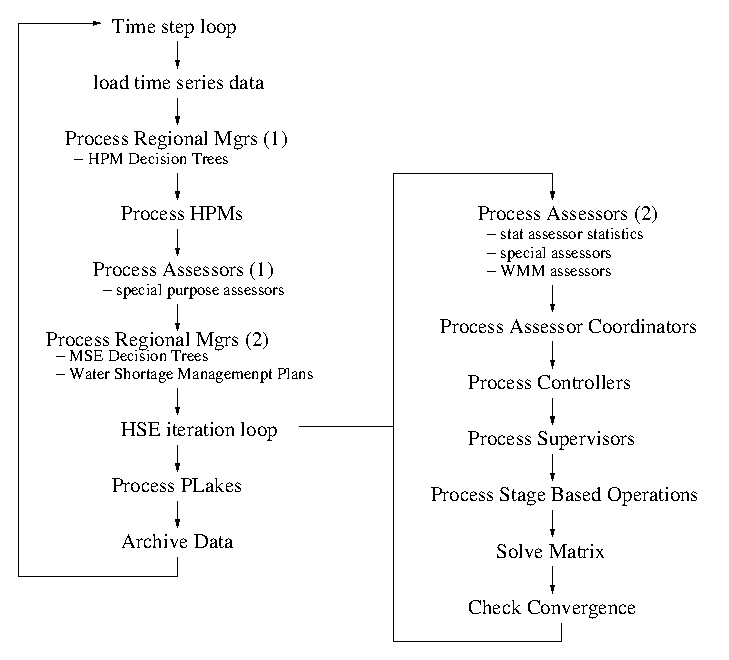
\includegraphics[scale=.8]{Graphics/regMngrFlowchart.eps}
 \end{center}
 \caption{\label{rsmFlowchart} RSM Process Flowchart.}        
\end{figure}

\section{Water Shortage Management Plan}

The area serviced by Lake Okeechobee, collectively known as the Lake
Okeechobee Service Area (``LOSA'') is comprised of four basins: North
Shore, Caloosahatchee River, St Lucie River, and the Everglades
Agricultural Area (``EAA'').  Lake Okeechobee is the primary source of
irrigation for these basins.  Following the one of the most severe
droughts on record in 1981, the District implemented the Water
Shortage Plan in 1982.  The plan provides specific guidelines for
water restrictions based on use type and severity of drought.  The
required water use restriction in the Lake Okeechobee Service Areas
are assumed to have been met if users comply with cutbacks as defined
in the Supply-Side Management (``SSM'') Plan (Hall, 1991).  

The Water Shortage Management Plan for Lake Okeechobee was revised
following the 2000-2001 drought.  A phased approach, based on forecast
Lake stage on June 1st was used.  This approach has been extensively
simulated with the SFWMM and is referred to as the existing Water
Supply Trigger or ``WST'' method.  

The District initiated rule development in February, 2006 to change
the existing water shortage rule to reflect 1-in-10 LOSA demands and
phased cutback approach.  The 1-in-10 year demands are based on SFWMM
simulations.  This approach is referred to as Lake Okeechobee Water
Shortage Management or ``LOWSM''.

Water shortage plans for Lake Okeechobee have been implemented in RSM
as regional managers.  The water supply demand in LOSA is computed for
each basin by their respective water supply assessors.  If the Lake is
under drought conditions (i.e., water levels are low enough to trigger
water restrictions), water supply releases through the outlets are
cutback by setting management constraints for water supply.

Water shortage management plan packages have been developed for
``SSM'' and ``LOWSM''.  Descriptions of the plans and parameter
specifications are provided in the following sections.

\subsection { {\tt ssm} package }

The Supply Side Management (SSM) package interfaces with the SSM
module which is a stand alone subroutine written in FORTRAN.  The SSM
module runs on a daily time step and requires as input stage in the
lake, stage from the SSM schedule and total regional demand from LOSA.
In return, SSM provides the cutback level to be applied to all water
supply releases to LOSA.  The cutbacks are imposed as management
constraints on the respective water supply outlets.

The SSM method calculates weekly allocations during water shortage
based on available volume in the Lake above a reference elevation
(11.0 ft).  The cutback varies based on date relative to June 1 and
the stage of Lake.  The maximum cutback is limited to 67 \%.


\subsection { {\tt lowsm} package }

The Lake Okeechobee Water Shortage Management package uses a phased
approach based on preset lines (rule curves) for 15\%, 30\%, 45\% and
60\% cutbacks.  The respective cutbacks are applied as Lake water
levels drop below the rule curves.  Cutbacks are applied to 1in10 LOSA
demands computed using previous simulations of the SFWMM and imposed
as management constraints on the respective water supply outlets.


\section{Decision Tree Management}\label{Section:DecisionTreeManagement}

The RSM provides a mechanism whereby the modeler can formulate
management constraints that will applied to selected structures using
decision trees. Lake regulation schedules are typically simulated
using ``management zones'' that prescribe an operational response for
a defined set of hydrologic criteria.  The collection of management
zones can be transformed into a decision tree structure, where
hydrologic conditions are tested against the hydrologic criteria of
each management zone to determine which (if any) of the prescribed
operations (i,e., constraints) should be deployed at the associated
structure.

Each management zone in a decision tree can consider multiple
hydrologic conditions using branches, where a branch tests a single
hydrologic criteria (see Figure \ref{flowchartDT}).  Depending on the
result of the test (true or false), the next hydrologic criteria is
tested.  The tests continue until a terminal end of the decision tree
is reached and the specified flow value is imposed as a management
constraint for the associated structure.

\begin{figure}
 \begin{center}
  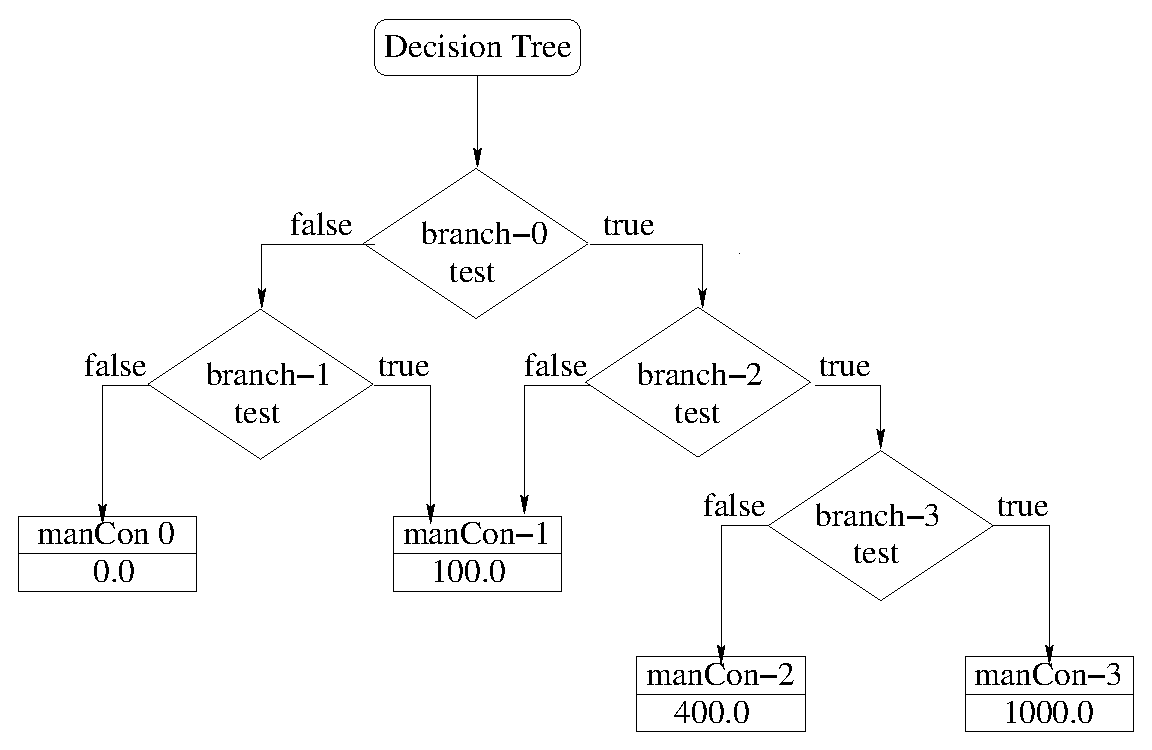
\includegraphics[scale=.45]{Graphics/flowchartDT.eps}
 \end{center}
 \caption{\label{flowchartDT} Sample Decision Tree Flowchart.}        
\end{figure}

Each branch specification contains a conditional test to
determine whether or not the hydrologic criteria has been satisfied.
If true, the {\tt true} attribute provides traversal instructions to
the decision tree manager on where to go next.  Likewise, traversal
instructions are provided by the {\tt false} attribute if the
conditional test is false.  

The RSM decision tree mechanism provides a variety of conditional tests
that can be used to test hydrologic criteria and return a Boolean
result:

\begin{enumerate}

 \item TBTest \-- the monitored value is tested against a management
 zone defined by a top and bottom rule curves.  If monitored value is
 between top and bottom, return true, otherwise return false.

 \item ABInequalityTest \-- a specified inequality (e.g., GT, GE, LT,
 LE) is used to compare a monitored value (A) with a rule curve value
 (B).  The result of the inequality test is returned.

 \item InequalityTest \-- a specified inequality (e.g., GT, GE, LT,
 LE) is used to compare a monitored value with a specified constant.
 The result of the inequality test is returned.

\end{enumerate}

The true and false traversal instructions in a branch have two parts.
The first part is either ``branch'', which indicates the next stop is
a branch, or ``manCon'', which indicates the next (and last) stop is a
management constraint.  The second part of the traversal instructions
is an integer that identifies the branch or manCon that will be processed
next. This integer must match the identification number of one of the
nested elements in decisionTree.

A management constraint is imposed on structure flow by different
processes, depending on the management method used in the RSM
implementation.

\begin{itemize}
 \item Assessor Coordinator. Every structure managed by the Assessor
   Coordinator is referenced through an MSE Node. Each MSE node
   includes management constraint variables whose values are updated
   through the deployment of MSE decision trees. The flood control and
   water supply assessors (``WCU assessors'') impose these management
   constraint variables through the course of their assessment. Since
   the WCU assessors distinquish between different purposes in their
   operational decision making, the management constraints variables
   are likewise dedicated for different purposes (e.g., flood control,
   water supply or environmental).

 \item Hydrologic Process Module. The base class for the hydrologic
   process model (HPModule) includes variables for management
   constraints whose values are updated through the deployment of HPM
   decision trees. Although these management constraint values are
   available to types of HPMs, the constraints are not applied
   generically across the HPModule classes. Currently, only the
   ModifiedSCS HPM has the capability to impose HPM decision tree
   constraints. The ModifiedSCS HPM supports the imposition of
   management constraints for flood control structure, pump and
   boundary conditions flows.

 \item Generic assessor. The MSE and HSE decision trees impose
   management constraints on flows managed within the context of
   assessor coordinators and ModifiedSCS HPMs, respectively. Other
   management methods, such as special assessors, user controllers and
   stage based operations have their own specialized ways of managing
   flows that rely on monitors to specify constraint values. Stat
   Assessor decision trees work the same as the MSE and HSE decision
   trees except they ``hold'' the management constraint variable and
   make available to other management processes through an assessor
   monitor.
\end{itemize}

The flow value used to set the management constraint can be defined by
a variety of ways.  The value or the method used to compute the value
is generally specified by the regulation schedule, policy, or
management plan simulated by regional manager.  Frequently, the
management constraint is a constant value. If the management
constraint varies by calendar date, a rule curve can be specified with
a rule curve monitor.  Other management constraints are computed,
based on the state of the system coupled with management parameters
specified by the user to simulate operational controls.  Special
purpose assessors are available to compute management constraint
values based on the current state of the system using computational
methods specified by the regulation schedule, policy or management
plan simulated by the regional manager.  These values are computed
before the regional managers are processed and access to their
computed values is provided through an assessor monitor.  Chapter
\ref{Chapter:specialPurposeAssessor} provides a description of the
special purpose assessors that can be used in conjunction with
regional managers.



 \section{Special Purpose Assessors}\label{Chapter:specialPurposeAssessor}

Frequently an operational or management decision depends on the
outcome of a specific assessment or calculation.  The RSM addresses
this need through special purpose assessors.  These assessors range
complexity, from a simple statistic, to an operational rule, to a
fully developed hydrologic model.  At construct time, the special
purpose assessor is supplied with user defined parameters and state
variable monitors that it needs to make its assessment.  The results
of its assessment are available through an assessor monitor.

Special purpose assessors are processed right after Hydrologic Process
Modules (HPM) but before Regional Managers (see Figure
\ref{rsmFlowchart}).  Therefore, all special purpose assessors
calculations are based on beginning of time step state variables with
the exception of HPM variables.


 \subsection{Back Pump Operation}

Flood control operations that discharge excess from an EAA basin to
Lake Okeechobee (commonly referred to as backpumping) are controlled by
the volume of runoff in the basin.  In general, backpumping is avoided
until runoff reaches a critical level.  The {\tt thresholdfrac}
package computes backpumped flow based on the following criteria:

\begin{equation}
	Q_{bp} = 0.0, \qquad Q_{runoff} \le Q_{thresh}
\end{equation}

\begin{equation}
	Q_{bp} = (Q_{runoff} - Q_{thresh}) * frac, \qquad Q_{runoff} > Q_{thresh}
\end{equation}

where:

\begin{center}
\begin{tabular}{rcl}
	$Q_{bp}$	&=& backpumped flow (cfs)					\\
	$Q_{runoff}$	&=& basin runoff (cfs)						\\
	$Q_{thresh}$	&=& threshold basin runoff (cfs)				\\
	$frac$		&=& fraction of basin runoff above threshold to be backpumped	\\
\end{tabular}
\end{center}

Backpumping operations are typically implemented by a Regional Manager
(see Chapter \ref{chapter:RegionalManager}) where the backpumping flow
computed by this assessor is monitored by an assessor monitor and used
to set a management constraint for flood control.  The decision tree
tests if the lake is above a specified backpump level \-- if it is,
set the management constraint to 0.0, otherwise, set the management
constraint to the backpump flow computed by this assessor.


 \subsection{Hysteresis Switch}

Hysteresis can be used to filter signals so that the output reacts
slowly by taking recent history into account.  For example, a
controller may turn on a pump when the water level drops below level
A, but not turn it off until the water level rises above level B.
This controller has hysteresis.  Thus the on/off output of controller
to the pump when the water level is between A and B depends on the
history of the water level.  This prevents rapid switching on and off
as the water levels drift around the set point.

The Hysteresis Switch assessor approximates the behavior of a
hysteresis controller, where a water level monitor is used as a signal
with specified on and off water levels.  The relative position of the
ON and OFF levels (Figure \ref{fig:HysteresisSwitch}) determines if
the pump is turned on when water levels drop below the ON level (``OFF
on top'') or when water levels rise above the ON level (``ON on
top'').

\begin{figure}[!htb]
 \begin{center}
  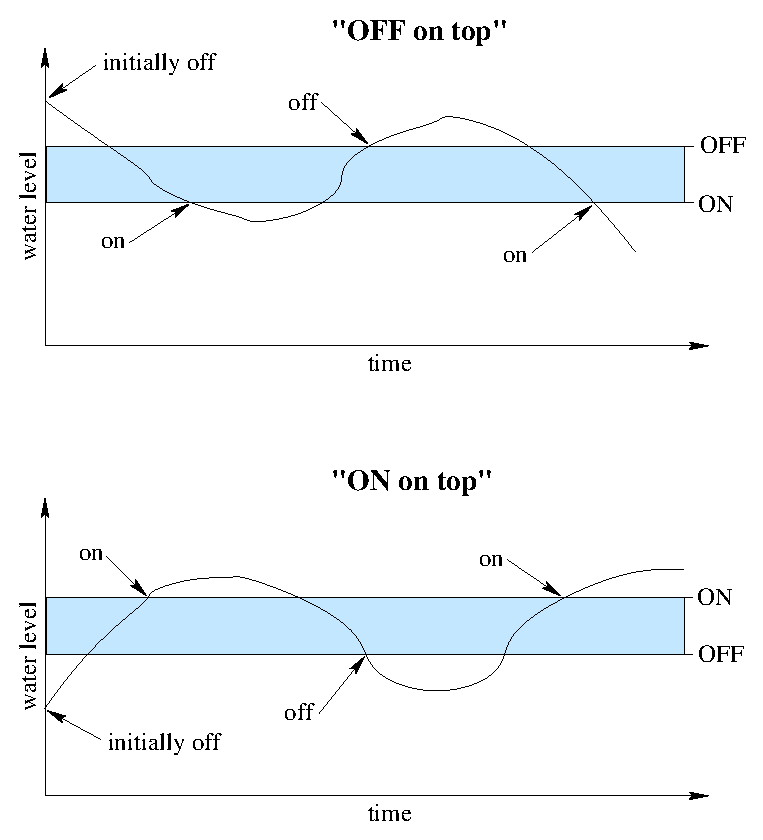
\includegraphics[scale=.5]{Graphics/hysteresis}
  \caption{\label{fig:HysteresisSwitch} Relative position of ON and OFF levels for the {\tt HysteresisSwitch} assessor.}
 \end{center}
\end{figure}

The Hysteresis Switch is typically used by a regional manager
to control the operation of a pump.  The output from the Hysteresis
Switch assessor is 0.0 (off) or 1.0 (on) and can be monitored using an
assessor monitor with the attribute set to ``flow''.

 \include{assessors/linearizeWM}
 \subsection{Pulse Release}
The {\tt std} flood control assessor includes a {\tt pulse} option
to simulate the pulse releases from a lake through selected flood
control outlets (see Section \ref{fcassessor:std}).  The {\tt pulse}
option is used to control flood releases to environmentally sensitive
areas such as estuaries where salinity levels are important.  Studies
have shown that flow discharges into estuaries should simulate the
natural stormwater runoff which occurs in a pulsing discharge manner.
Discharges at the designated outlet follow a predefined flow
hydrograph for a specified number of days.

The {\tt pulse} option manages pulse releases from multiple outlets
(e.g., S77 to the Caloosahatchee Estuary and S308 to the St Lucie
Estuary).  The pulse release properties for each outlet are defined in
{\tt pulseRelease} special purpose assessor.  The {\tt pulse} option
refers to each {\tt pulseRelease} by specifying their respective
asmtID.

The {\tt pulseRelease} assessor supports multiple levels with flow
hydrographs that approximate the hydrologic response of a drainage
basin to storms of varying intensities.  This feature enables lake
managers to initiate a particular pulse level depending on the
severity of the flood control condition of the Lake.  The pulse
release levels are defined by multiple {\tt pulseHydrograph}
entries.

A pulse release can be initiated in two ways.  The standard option is
based only on lake stage.  A pulse release zone is associated with
each {\tt PulseHydrograph}.  The zone is defined by top and bottom
rulecurves and if the lake stage falls within the zone, a pulse
release is initiated.  For each day in the pulse release period, the
outlet release is determined by the pulse release hydrograph.  Once
initiated, the pulse release is completed, even if the lake stage falls
outside the zone.

The second option for initiating a pulse release relies on a wse
schedule defined by a regional manager.  The Water Supply and
Environmental (WSE) Schedule was developed to manage flood control
releases for Lake Okeechobee, considering a local and global climatic
influences.  This option uses a decision tree manager to assess the
condition of the lake. The decision tree manager traverses through a
collection of decision branches and until it reaches a terminal point
where a management constraint is defined for an mseNode.  The WSE
Decision Tree specifies pulse release at several terminal points.
These points are assigned to management constraints.  The wse {\tt
pulseHydrograph} package accesses the decision tree manager to
determine which (if any) pulse release should be initiated.  As with
the standard pulse release, once pulse release has been initiated,
outlet releases are set by the pulse hydrograph for the duration of
the pulse period.


 \subsection{Statistic Assessor}

The {\tt statassessor} assessor has two modes of operation. By
default, the {\tt statassessor} calculates a basic statistic for a
collection of time series monitors.  The following statistics are
computed using the specified attribute:

\begin{enumerate}
 \item sum \-- summation
 \item ave \-- average
 \item min \-- minimum 
 \item max \-- maximum
\end{enumerate}

The second mode uses the package attribute to specify an alternative
statistic or special calculation. These packages are described in the
following sections.


 \subsubsection{{\tt fc2estuary} package}

The {\tt fc2estuary} package was developed to manage flood control
releases from a canal where the inlet is connected to reservoir with
potentially large flood control releases (e.g., Lake Okeechobee), the
outlet is connected to an estuary, and the canal receives runoff from
adjacent basins.  The assessor executes the flood control assessor for
upstream water control unit (Lake Okeechobee) and retrieves flood
control release computed for the inlet to the canal.  The assessor
compares this value to the runoff from the adjacent basins, and uses
the bigger value to set the maximum release to the estuary.
Typically, this value is used by a Regional Manager or LP Supervisor
to set a management constraint for flood control on the outlet to the
estuary.


\subsubsection{{\tt fc2estuary\_alt1} package}

The {\tt fc2estuary\_alt1} package was developed to manage flood
control releases from a canal where the inlet is connected to
reservoir with potentially large flood control releases (e.g., Lake
Okeechobee), the outlet is connected to an estuary, and the canal
receives runoff from adjacent basins.  The assessor executes the flood
control assessor for upstream water control unit (Lake Okeechobee) and
retrieves flood control release computed for the inlet to the canal.
The {\tt fc2estuary\_alt1} package compares the basin runoff with the
Lake regulatory release, and returns the larger value only when the
Lake is making a pulse release or a base flow.  Otherwise, {\tt
  fc2estuary\_alt1} returns the sum of basin runoff and Lake
regulatory release.  Typically, the return value is used by a Regional
Manager or LP Supervisor to set a management constraint for flood
control on the outlet to the estuary.  

\subsubsection{{\tt fc2estuary\_alt2} package}

The {\tt fc2estuary\_alt2} package was developed to manage flood
control releases from a canal where the inlet is connected to
reservoir with potentially large flood control releases (e.g., Lake
Okeechobee), the outlet is connected to an estuary, and the canal
receives runoff from adjacent basins.  The assessor executes the flood
control assessor for upstream water control unit (Lake Okeechobee) and
retrieves flood control release computed for the inlet to the canal.
The {\tt fc2estuary\_alt2} package compares the basin runoff with the
Lake regulatory release, and returns the larger value for any Lake
regulatory release, including base flows, pulse release and standard
regulatory releases.  Typically, the return value is used by a
Regional Manager or LP Supervisor to set a management constraint for
flood control on the outlet to the estuary.  

 \subsubsection{{\tt TwoPointInterp} package}

Water levels in WCU's are commonly managed through regulation
schedules, where structure operations are based on the state of the
system and calendar date.  A regulation schedule is comprised of
``management zones'' that prescribe an operational response for a
defined set of hydrologic criteria (see Section
\ref{Section:DecisionTreeManagement}).  If the value returned by a
target monitor falls between the management zone's top and bottom
rulecurves, a management constraint (manCon) is set to a specified
value.  The {\tt TwoPointInterp} package is used to set the manCon to
a value based on the relative position of the target value in the
range defined by the two rulecurves.  The manCon values associated
with each rulecurve are combined by a weighting function:

\begin{align}
  weight &= 1.0,& target &\ge rulecurve_B \\
  weight &= \frac{target - rulecurve_C}{rulecurve_B - rulecurve_C},& rulecurve_B &> target > rulecurve_C \\
  weight &= 0.0, &target &\le rulecurve_C 
\end{align}

where 
\begin{center}
\begin{tabular}{rcl}
	$weight$	&=& weighting factor					\\
	$target$	&=& monitored time series value				\\
	$rulecurve_B$	&=& top value of the range				\\
	$rulecurve_C$	&=& bottom value of the range				\\
\end{tabular}
\end{center}

The weighted manCon value is computed by:

\begin{equation}
	value_{weighted} = weight * manCon_B + (1-weight) manCon_C
\end{equation}

where 
\begin{center}
\begin{tabular}{rcl}
	$manCon_B$	&=& managed constraint value for $rulecurve_B$	\\
	$manCon_C$	&=& managed constraint value for $rulecurve_D$	\\
\end{tabular}
\end{center}


 \subsection{Water Control Unit Status}

The status of a water control unit can be assessed using a {\tt
  WcuStatus} assessor.  In particular, {\tt WcuStatus} assessors are
used to compute the water supply deficit and flood control excess for
a water control unit.

The water supply deficit is defined as the volume of water required to
raise the water level up to a target deficit level.  The computed
deficit includes the net contribution of the HPM.  The flood control
excess is the volume of water required to lower the water level down
to a target flood control.  The computed excess includes net
contributions of the HPM, inlet inflows, unmanaged outlet releases,
outlet water supply releases, and boundary flows.  

The {\tt wcuDeficit} and {\tt wcuExcess} modes were designed to assess
the water supply and flood control status of basins and lakes.  The
{\tt canalExcess} mode was developed to designed to assess the flood
control status of particular type of water control unit \-- an EAA
canal.  The excess in an EAA canal is computed by executing the flood
control assessors assigned to the agricultural and stormwater
treatment areas, and reservoirs adjacent to the EAA canal.  Canal
excess is the summation of flood control releases through the
respective outlets to the EAA canal.  

% \include{monitors/monitors}
% \include{monitors/monitor_hse}
% \include{monitors/monitor_waterbody}
% \include{monitors/monitor_hpm}
% \include{monitors/monitor_wm}
% \include{monitors/monitor_mse}

\bibliographystyle{plain}
\bibliography{usersGuideRsmbn}

 \end{document}
